%%%%%%%%%%%%%%%%%%%%%%%%%%% START WITH LATEX PREAMBLE %%%%%%%%%%%%%%%%%%%%%%
% reminder: its = possessive
%           it's = it + is

%use [11pt, draft] for draft markings.
\documentclass[11pt]{mvlthesis}
%\documentclass[16pt, draft]{mvlthesis}
\usepackage[dvipdfm]{graphicx}
\usepackage{verbatim,amssymb,amsmath}
\usepackage{float}
%\usepackage{epstopdf}
%\usepackage{afterpage}
\graphicspath{ {images/} }

%%%%%%%%%%%%%%%%%%%%% SET UP ALL THE TITLE PAGE VARIABLES %%%%%%%%%%%%%%%%%%

\title{\scshape \mbox{THESIS OR DISSERTATION TITLE}\\
\scshape \mbox{TITLE LINE 2}}

\author{Travis F. Collins}
\thesis_or_diss{Thesis}
\degree_type{Master of Science}
\field{Electrical and Computer Engineering}
\degreeyear{December 2012}
\chair{Professor Alexander Wyglinski}
\chairtitle{Major Advisor}
\membertwo{Professor Y}
\memberthree{Professor Z}

%%%%%%%%%%%%%%%%%%%%%% INCLUDE USER DEFINED COMMANDS %%%%%%%%%%%%%%%%%%%%%%%

\newcommand{\bi}{\begin{itemize}}
\newcommand{\ei}{\end{itemize}}
\newcommand{\ii}{\item}
\newcommand{\be}{\begin{enumerate}}
\newcommand{\ee}{\end{enumerate}}
\newcommand{\ie}{\item}

\newcommand{\fig}[5]{
    \begin{figure}[#1]
    \begin{center}
    \includegraphics[#2]{#3}
    \end{center}
    \caption{#4}
    \label{#5}
    \end{figure}
}

%\frenchspacing

%%%%%%%%%%%%%% SPECIFY WHICH PARTS OF THE THESIS YOU WANT PRINTED %%%%%%%%%%

\renewcommand{\baselinestretch}{1.5}

\newcommand{\pderiv}[2]{\mbox{$\frac{\displaystyle \partial #1}{\displaystyle \partial #2}$}}

%%%%%%%%%%%%%%%%%%%% Done with setup, document starts here %%%%%%%%%%%%%%%%%
\begin{document}


%%%%%%%%%%%%%%%%%%%%%%%%%%%%%% TITLE + ABSTRACT %%%%%%%%%%%%%%%%%%%%%%%%%%%%
\maketitle
\begin{abstract}

Since the advent of modern digital communications in the 20th century there has been an explosion in the demand for wireless spectrum. As a result spectrum is becoming an increasingly scare resource. This demand is a direct result of the availability and relatively inexpensive cost of such wireless device. Therefore in such environments as militaristic theatres the probability of interfering transmissions, intended and unintended, has steadily grown to a point where techniques need to be consider to combat such occurrences. More directly, in such situations when interfering signals are partially or completely understood measures can be taken to overcome such difficulties. Under these assumptions several well know techniques are can be applied to combat such scenarios.  This research analyzes the feasibility of combining Antenna Subset Selection, Spectral Subtraction, and Blind Source Separation signal processing techniques to accomplish this goal.  Together they provide multiple avenues of signal separation to remove such jamming effects, for both narrow and wide bands, without hindering the mobility of the nodes themselves.


\end{abstract}

%%%%%%%%%%%%%%%%%%%%%% ACKNOWLEDGMENTS + TABLE OF CONTENTS %%%%%%%%%%%%%%%%%

\begin{frontmatter}

\begin{acknowledgements}
%\begin{center}
%\vspace{0.4in}
%\end{center}
\end{acknowledgements}
\tableofcontents
\listoffigures
\listoftables

\end{frontmatter}

%%%%%%%%%%%%%%%%%%%% INCLUDE THE REST OF THE DOCUMENT %%%%%%%%%%%%%%%%%%%%%%


%\section{Motivation}

Since the advent of modern digital communications in the 20th century there has been an explosion in the demand for wireless spectrum.  As a result spectrum is becoming an increasingly scare resource\cite{scarcity}.  This demand is a direct result of the availability and relatively inexpensive cost of such wireless device.  Therefore in such envirorments as militaristic theatres the probability of interfering transmissions, intended and unintended, has steadily grown to a point where techniques need to be consider to combat such occurrences.  More directly, in such situations when interfering signals are partially or completely understood measures can be taken to overcome such difficulties.\\

In military theatres it is extremely common to observe friendly operated high-power broadband jamming signals\cite{frater}.  Such devices exists as part of group convoys in several branches of the military and in many other forms in contested territories or war-zones.  Unfortunately such devices block both friendly and hostile communications, and current anti-jamming techniques haven't provided a viable solution to this problem.  Therefore new avenues should be considered, utilizing more flexible radio technologies.\\

Understanding how to overcome such challenges is a complex task; with vastly different transmission envirorments and differing operating devices and operating standards.  A new system that could combat such downfalls should rely on all friendly information, or be able to construct solutions of its own from a set of tools given to the radio.  Such tools should be flexible and easily modified, changed, or improved.  This ability to easily change or adapt is a key feature as the technical requirements can change from day to day, or between branches of the military itself. As such a solution should have the following attributes:

\begin{itemize}
\item \textbf{Flexible:}

\item \textbf{Resilient:}

\item \textbf{Hardened:} in changing enviroments

\end{itemize}


\section{State of the Art}

Current implementations in anti-jamming technology lies on the strateling point of hardware and software in the communications world.  This is true because hardware provides the speed and performance needed for digital data transmission, while software provides higher level intelligence and flexibility in such layers as the media access control layer and the network layer of the Open Systems Interconnect (OSI) model\cite{Zimmermann}.  For anti-jamming applications, high intelligence allows for mobility again the jammer.  Therefore a large implementation in software must be considered when investigating anti-jamming technics.\\

%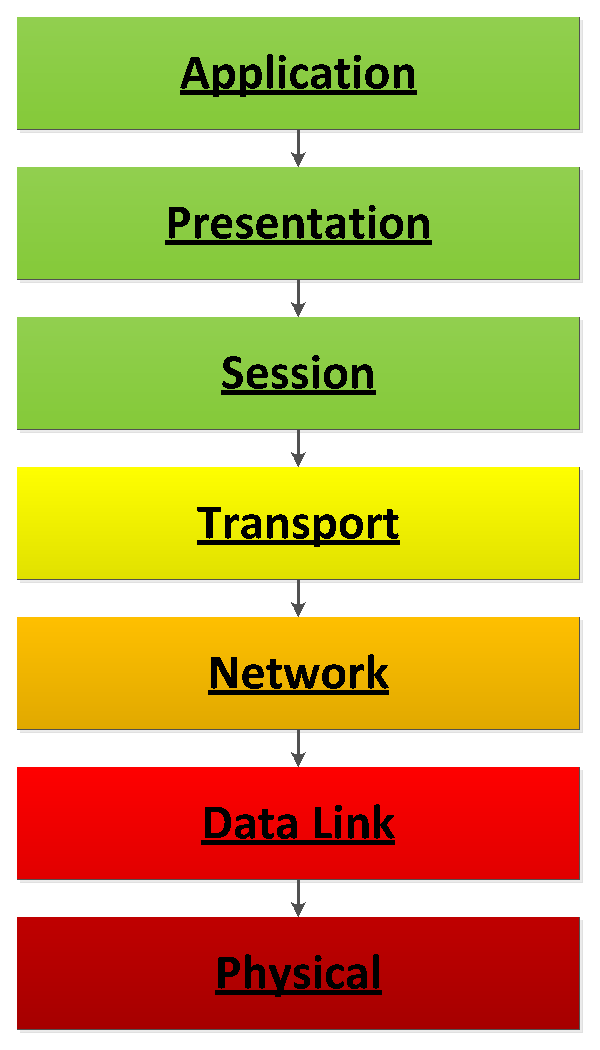
\includegraphics[width=60mm]{OSI_model.eps}
%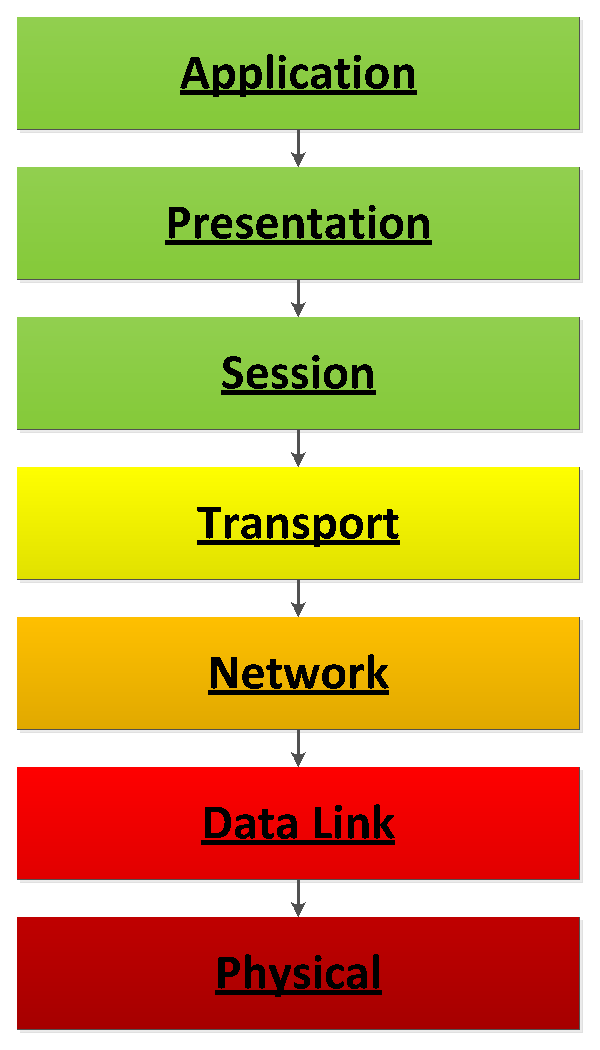
\includegraphics[height=60mm]{OSI_model.eps}
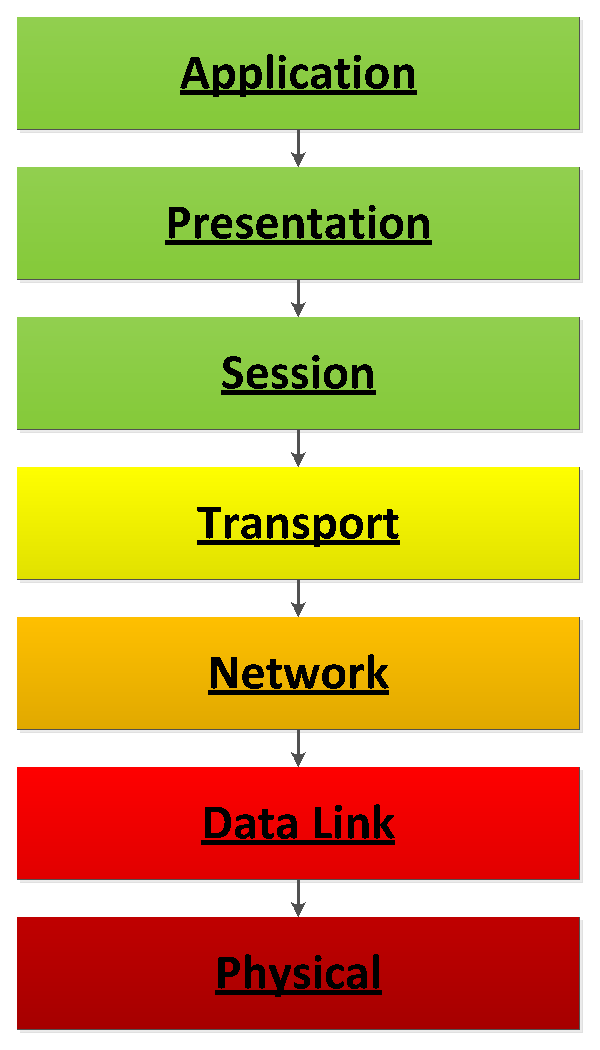
\includegraphics[scale=0.10]{OSI_model.eps}
%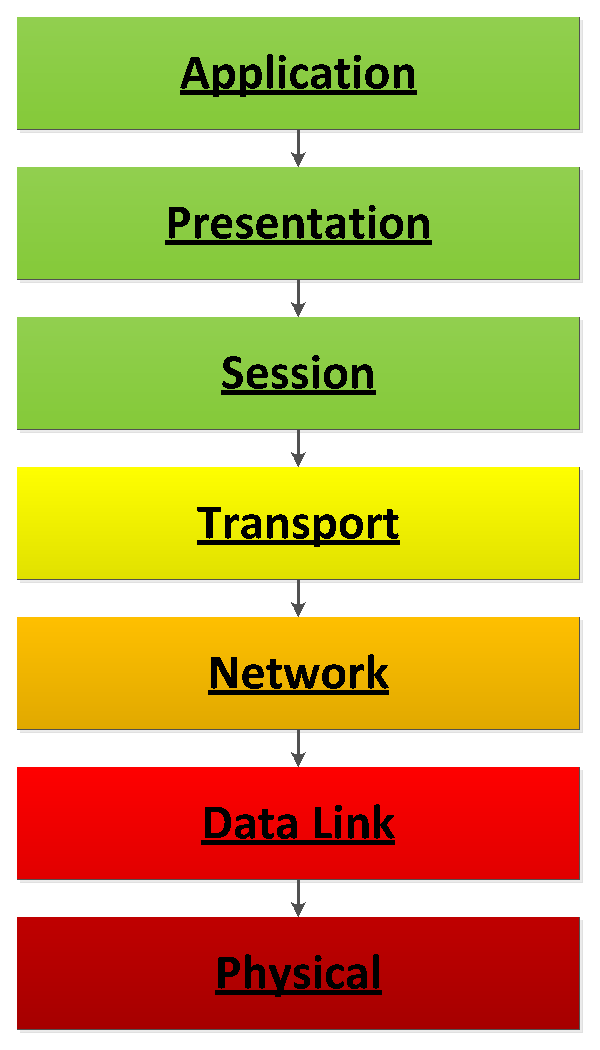
\includegraphics[angle=45,width=52mm]{OSI_model.eps}

Current anti-jamming technics include channel hopping, spatial retreat, jammed area mapping, node escape, retreat restoration, frame masking, and many more\cite{1}.  All of these techniques use mechanisms of evasion or despection.  These can be quite effective when attacked by generally narrowband, non-dynamic/non-learning jammers.  In the case of wide and ultra-wide band jammers, they fail miserably.  This wide-band enviorment is the primary situation of interest, and it generally considered a hopeless scenario.  These anti-jam technics are design for specific situations and jammers.\\

Let us first examine these anti-jamming technics which are broken down into three primary categories: Proactive countermeasures, Reactive countermeasures, and Mobile agent-base countermeasures\cite{1}.  Reactive countermeasures relies on a varying array of detection mechanisms first to determine if that node is being jammed.  These detection methods  must be coupled with a countermeasure or the scheme is in operable.  Examples of these detection methods include a transmitter-based approach and a receiver-based detection.  In a transmitter-based approach, such as ad-hoc networks, a decision algorithm is used based on four metrics: Packet Delivery Ratio (PDR), Received Signal Strength Indicator (RSSI), Physical rate, and Noise levels\cite{3}.  In the receiver-based detection additional information must be injected into frames to help the receiver determine the number of frames lost.  Since frames can be easily lost in wireless transmissions, the receiver is handicapped when determining the number of retransmissions that have occurred.  In the transmitter the PDR is deterministicly determined by the data-link layer, sequence numbers must be added to frames for the receiver to accurately calculate the PDR\cite{3}.  Several other detection methods exist including using a detected detector, cooperative detection among nodes in a wireless network, and more sophisticated methods of RF fingerprinting\cite{3}.\\

Once the jammer has been detected the reactive countermeasures come into play.  Many evasion techniques exists to combat narrowband jammers such as: channel hoping, spatial retreat, retreat restoration, hybrid attacks, and many cognitive radio approaches\cite{2}.  Many of these technics utilize the network itself to adapt to the jammer, which is an appropriate assumpt because without a network communications are irrelivant.  Channel hopping is quite simple and can be considered easiet to implement.  If a channel is begining jammed simply ``hop'' to another channel.  This is easily defeated in two cases, the first the jammer follows you or the jammer is simply wideband capable.  The second, spatial retreat, is a mechanism to physically evade the areas being jammed. Based on the detection algorithm all nodes in a network try to estimate the jammed region and flee physically in the direction of safer place. Based on their estimation about the jammed region, nodes will utilize shortest path algorithms to determine location of retreat\cite{5}.  Retreat restoration is focused around how to rebuild a network once the jammer has left.  Retreat restoration can be done by coordinated or uncoordinated communication, and the transmissions are based on a pre planned hop patterns among nodes\cite{6}.\\

There also exists systems that are design to resist jamming proactively.  These hybrid systems\cite{7} utilize preventatives measure to resist jamming such as frequency hopping spread spectrum (FHSS).  Spread-spectrum signals are highly resistant to narrowband jamming, unless the jammer has knowledge of the spreading key. In military applications the spreading key is generally created using a crytographic function\cite{sterling}.  More hybrid solutions include synchronous and asynchronous spectral multiplexing where intermediary nodes are used to communicate at multiple channels.  When a node changes its channel because of jamming a neighbor will heal that connection by communicating  with the node on its new channel and rest of the network on the old channel\cite{8}.


The largest problem with these techniques is they all have are designed to combat narrowband jammers, and even friendly jammers.  If high powered wideband jammers enter the equation, all of these solutions fall apart.  Note these techniques primarily exploit the dimensionality of their envirmonent by simply avoiding the jammer, and all techniques require intelligent flexible hardware solutions.   To implement such solutions requires suffisticated hardware implementations, that can be quite rigid for rapidly changing communication envirorments and adversaries.  To compensate solutions that push more of the radio operations from their original rigid hardware implementations into the more flexible software domain, provide a more cost effective and elligent solution.  These software focused radios, also know as Software defined radios, have provided a solid platform for very adaptive anti-jamming technologies under the name cogntive radios.  These radios have the ability to easily learn and adapt to their envirorment, which is the primary requirement of anti-jamming devices.\\

As mentioned above, it is quite common for the military to self-jam its own channels.  Unfortunately this can hinder their own use unintenially.  These disrupted users are known as ``disadvantage users''.  They are commonly small mobile hand held devices and cannot simply overcome the jammer computationally or in raw power; therefore, more manageable and eligent solutions must be considered for such disadvantaged users.  Beside self-jammming, adversarial jammers must also be considered.  Fortunately certain characteristics can be statistically exploited if these jammer abide by certain properties. Since adversarial jammers tend to inject random data or energy to block communication, if these transmissions can be shown to repeat they can be exploited.  In the case of self-jamming, the signal characteristic can be know \textit{a priori}; therefore they also can exploted or removed, negating the effects of such devices.  Such scheme must consider the energy or symbols of the jammmer that are orthoganol and/or non-orthoganol to the symbols of the communication itself.\\


The goal of this project is to exploit a self-jammed and statiscially determistic adversarially jammed channel, throught the utilization of cognitive radio, implemented on a software defined radio platform.  Software defined radios, defined as the intersection between hardware radios and computer software\cite{4}, provide a platform flexible enough to support highly intelligence operations such that anti-jamming requires.  A proposed adaptive signal processing software solution for mitigating the effects of both intentional and unintentional jamming (including wideband jamming) via the combination of antenna subset selection, spectral subtraction, and blind source separation (BSS) techniques in order to extract specific transmissions from a mixture of intercepted wireless signals. The goal of our proposed solution, called BLInd Spectrum Separation (BLISS), is to enable reliable, high throughput, and robust end-to-end wireless communications.\\

\section{Thesis Contributions}

This thesis will contribute the following to the wireless communications and signal processing research communities:

\begin{itemize}
\item A basis for blind source separation of define subset of signals, and tools on estimating and removing those signals.

\item A practical implementation using over the air communications of a anti-jamming sytem utilizing software defined radios. This implementation will tackle wideband non-orthoganol and orthoganol jamming, and provide evidence of probability of operational.
\end{itemize}


\section{Thesis Organization}

This thesis will be organized into the following chapters.  Chapter 2 provides the necessary background to understand basic communication system design, anti-jamming technics, and signal processing.  Chapter 3 puts forward a theoritical simulations and a design of a physical anti-jamming system.  Chapter 4 presents the results of the physical implement and analysis of its findings.  Chapter 5 concludes the thesis, summarizing the accomplishments and outlines possible future work.

\section{Motivation}

Since the advent of modern digital communications in the 20th century there has been an explosion in the demand for wireless spectrum.  As a result spectrum is becoming an increasingly scare resource\cite{scarcity}.  This demand is a direct result of the availability and relatively inexpensive cost of such wireless device.  Therefore in such envirorments as militaristic theatres the probability of interfering transmissions, intended and unintended, has steadily grown to a point where techniques need to be consider to combat such occurrences.  More directly, in such situations when interfering signals are partially or completely understood measures can be taken to overcome such difficulties.\\

In military theatres it is extremely common to observe friendly operated high-power broadband jamming signals\cite{frater}.  Such devices exists as part of group convoys in several branches of the military and in many other forms in contested territories or war-zones.  Unfortunately such devices block both friendly and hostile communications, and current anti-jamming techniques haven't provided a viable solution to this problem.  Therefore new avenues should be considered, utilizing more flexible radio technologies.\\

Understanding how to overcome such challenges is a complex task; with vastly different transmission envirorments and differing operating devices and operating standards.  A new system that could combat such downfalls should rely on all friendly information, or be able to construct solutions of its own from a set of tools given to the radio.  Such tools should be flexible and easily modified, changed, or improved.  This ability to easily change or adapt is a key feature as the technical requirements can change from day to day, or between branches of the military itself. As such a solution should have the following attributes:

\begin{itemize}
\item \textbf{Flexible:}

\item \textbf{Resilient:}

\item \textbf{Hardened:} in changing enviroments

\end{itemize}


\section{State of the Art}

Current implementations in anti-jamming technology lies on the strateling point of hardware and software in the communications world.  This is true because hardware provides the speed and performance needed for digital data transmission, while software provides higher level intelligence and flexibility in such layers as the media access control layer and the network layer of the Open Systems Interconnect (OSI) model\cite{Zimmermann}.  For anti-jamming applications, high intelligence allows for mobility again the jammer.  Therefore a large implementation in software must be considered when investigating anti-jamming technics.\\

%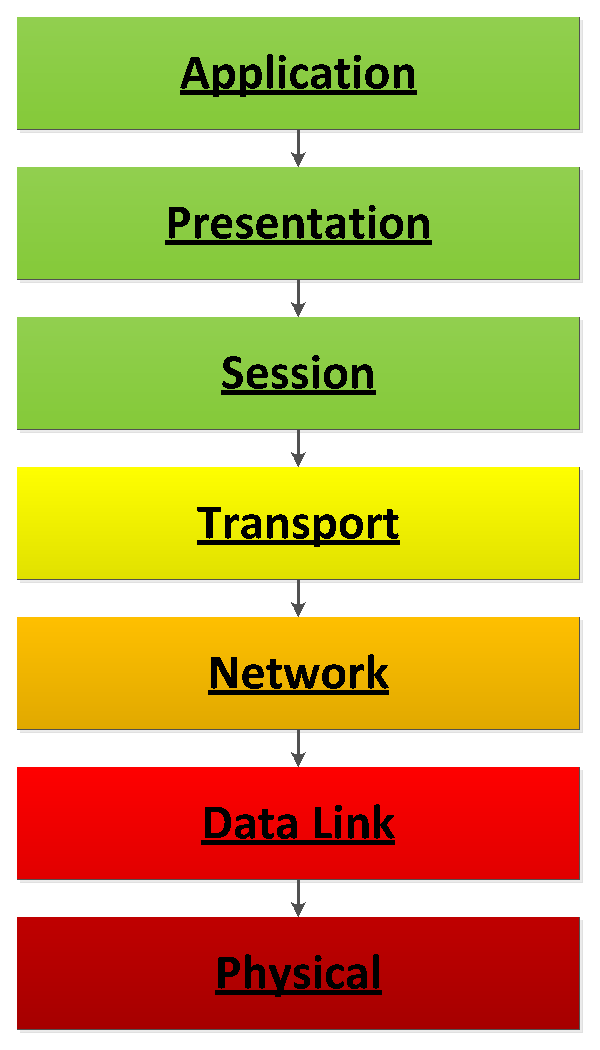
\includegraphics[width=60mm]{OSI_model.eps}
%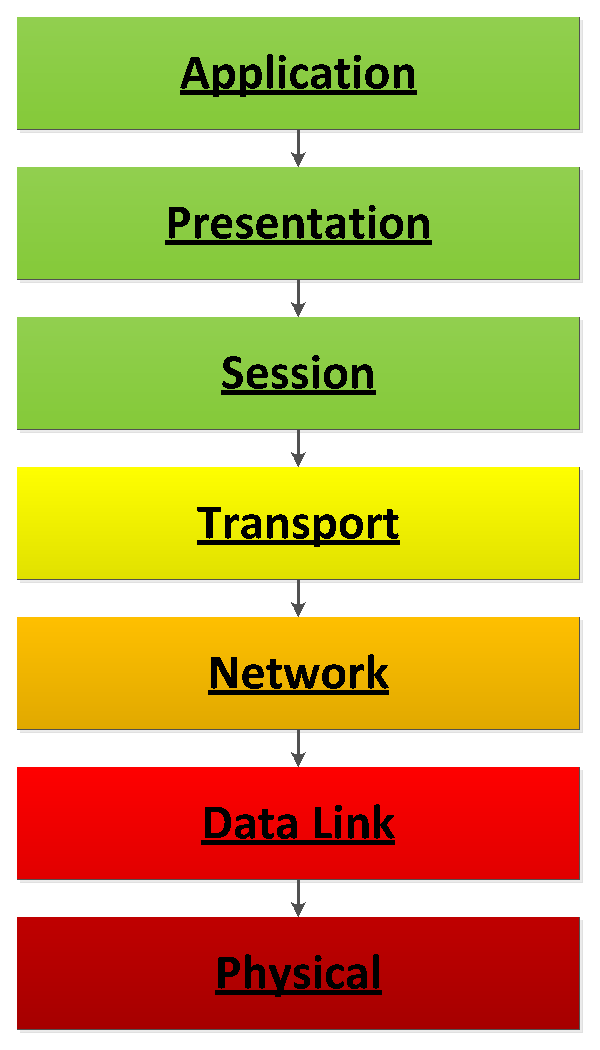
\includegraphics[height=60mm]{OSI_model.eps}
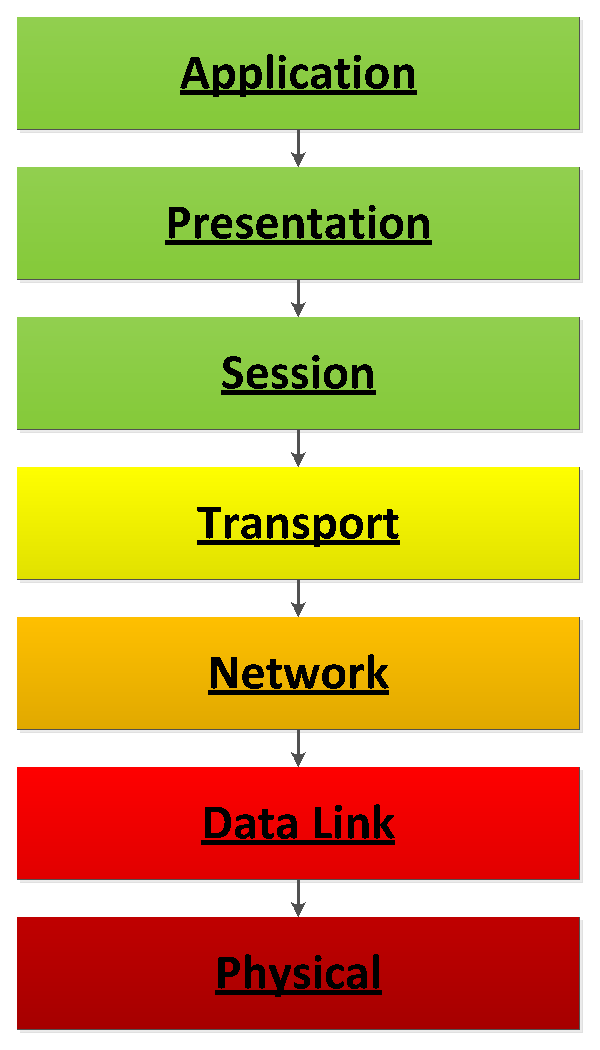
\includegraphics[scale=0.10]{OSI_model.eps}
%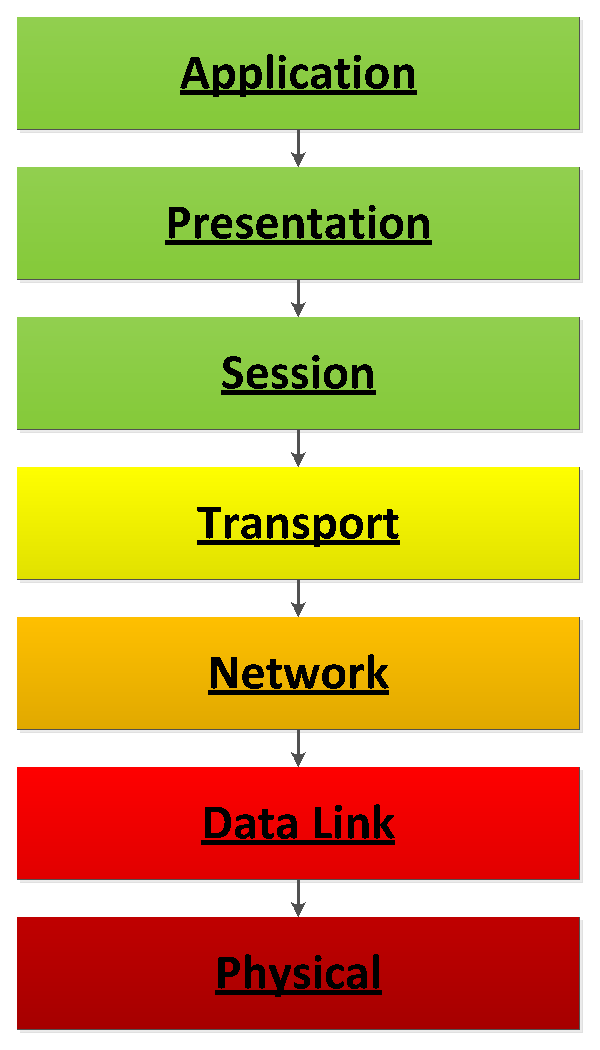
\includegraphics[angle=45,width=52mm]{OSI_model.eps}

Current anti-jamming technics include channel hopping, spatial retreat, jammed area mapping, node escape, retreat restoration, frame masking, and many more\cite{1}.  All of these techniques use mechanisms of evasion or despection.  These can be quite effective when attacked by generally narrowband, non-dynamic/non-learning jammers.  In the case of wide and ultra-wide band jammers, they fail miserably.  This wide-band enviorment is the primary situation of interest, and it generally considered a hopeless scenario.  These anti-jam technics are design for specific situations and jammers.\\

Let us first examine these anti-jamming technics which are broken down into three primary categories: Proactive countermeasures, Reactive countermeasures, and Mobile agent-base countermeasures\cite{1}.  Reactive countermeasures relies on a varying array of detection mechanisms first to determine if that node is being jammed.  These detection methods  must be coupled with a countermeasure or the scheme is in operable.  Examples of these detection methods include a transmitter-based approach and a receiver-based detection.  In a transmitter-based approach, such as ad-hoc networks, a decision algorithm is used based on four metrics: Packet Delivery Ratio (PDR), Received Signal Strength Indicator (RSSI), Physical rate, and Noise levels\cite{3}.  In the receiver-based detection additional information must be injected into frames to help the receiver determine the number of frames lost.  Since frames can be easily lost in wireless transmissions, the receiver is handicapped when determining the number of retransmissions that have occurred.  In the transmitter the PDR is deterministicly determined by the data-link layer, sequence numbers must be added to frames for the receiver to accurately calculate the PDR\cite{3}.  Several other detection methods exist including using a detected detector, cooperative detection among nodes in a wireless network, and more sophisticated methods of RF fingerprinting\cite{3}.\\

Once the jammer has been detected the reactive countermeasures come into play.  Many evasion techniques exists to combat narrowband jammers such as: channel hoping, spatial retreat, retreat restoration, hybrid attacks, and many cognitive radio approaches\cite{2}.  Many of these technics utilize the network itself to adapt to the jammer, which is an appropriate assumpt because without a network communications are irrelivant.  Channel hopping is quite simple and can be considered easiet to implement.  If a channel is begining jammed simply ``hop'' to another channel.  This is easily defeated in two cases, the first the jammer follows you or the jammer is simply wideband capable.  The second, spatial retreat, is a mechanism to physically evade the areas being jammed. Based on the detection algorithm all nodes in a network try to estimate the jammed region and flee physically in the direction of safer place. Based on their estimation about the jammed region, nodes will utilize shortest path algorithms to determine location of retreat\cite{5}.  Retreat restoration is focused around how to rebuild a network once the jammer has left.  Retreat restoration can be done by coordinated or uncoordinated communication, and the transmissions are based on a pre planned hop patterns among nodes\cite{6}.\\

There also exists systems that are design to resist jamming proactively.  These hybrid systems\cite{7} utilize preventatives measure to resist jamming such as frequency hopping spread spectrum (FHSS).  Spread-spectrum signals are highly resistant to narrowband jamming, unless the jammer has knowledge of the spreading key. In military applications the spreading key is generally created using a crytographic function\cite{sterling}.  More hybrid solutions include synchronous and asynchronous spectral multiplexing where intermediary nodes are used to communicate at multiple channels.  When a node changes its channel because of jamming a neighbor will heal that connection by communicating  with the node on its new channel and rest of the network on the old channel\cite{8}.


The largest problem with these techniques is they all have are designed to combat narrowband jammers, and even friendly jammers.  If high powered wideband jammers enter the equation, all of these solutions fall apart.  Note these techniques primarily exploit the dimensionality of their envirmonent by simply avoiding the jammer, and all techniques require intelligent flexible hardware solutions.   To implement such solutions requires suffisticated hardware implementations, that can be quite rigid for rapidly changing communication envirorments and adversaries.  To compensate solutions that push more of the radio operations from their original rigid hardware implementations into the more flexible software domain, provide a more cost effective and elligent solution.  These software focused radios, also know as Software defined radios, have provided a solid platform for very adaptive anti-jamming technologies under the name cogntive radios.  These radios have the ability to easily learn and adapt to their envirorment, which is the primary requirement of anti-jamming devices.\\

As mentioned above, it is quite common for the military to self-jam its own channels.  Unfortunately this can hinder their own use unintenially.  These disrupted users are known as ``disadvantage users''.  They are commonly small mobile hand held devices and cannot simply overcome the jammer computationally or in raw power; therefore, more manageable and eligent solutions must be considered for such disadvantaged users.  Beside self-jammming, adversarial jammers must also be considered.  Fortunately certain characteristics can be statistically exploited if these jammer abide by certain properties. Since adversarial jammers tend to inject random data or energy to block communication, if these transmissions can be shown to repeat they can be exploited.  In the case of self-jamming, the signal characteristic can be know \textit{a priori}; therefore they also can exploted or removed, negating the effects of such devices.  Such scheme must consider the energy or symbols of the jammmer that are orthoganol and/or non-orthoganol to the symbols of the communication itself.\\


The goal of this project is to exploit a self-jammed and statiscially determistic adversarially jammed channel, throught the utilization of cognitive radio, implemented on a software defined radio platform.  Software defined radios, defined as the intersection between hardware radios and computer software\cite{4}, provide a platform flexible enough to support highly intelligence operations such that anti-jamming requires.  A proposed adaptive signal processing software solution for mitigating the effects of both intentional and unintentional jamming (including wideband jamming) via the combination of antenna subset selection, spectral subtraction, and blind source separation (BSS) techniques in order to extract specific transmissions from a mixture of intercepted wireless signals. The goal of our proposed solution, called BLInd Spectrum Separation (BLISS), is to enable reliable, high throughput, and robust end-to-end wireless communications.\\

\section{Thesis Contributions}

This thesis will contribute the following to the wireless communications and signal processing research communities:

\begin{itemize}
\item A basis for blind source separation of define subset of signals, and tools on estimating and removing those signals.

\item A practical implementation using over the air communications of a anti-jamming sytem utilizing software defined radios. This implementation will tackle wideband non-orthoganol and orthoganol jamming, and provide evidence of probability of operational.
\end{itemize}


\section{Thesis Organization}

This thesis will be organized into the following chapters.  Chapter 2 provides the necessary background to understand basic communication system design, anti-jamming technics, and signal processing.  Chapter 3 puts forward a theoritical simulations and a design of a physical anti-jamming system.  Chapter 4 presents the results of the physical implement and analysis of its findings.  Chapter 5 concludes the thesis, summarizing the accomplishments and outlines possible future work.


%% Background Section
\chapter{Required Background Knowledge}
\label{ch:background}

This chapter provides the background information needed to understand the chapters that follow.  It examines the basic outline of a communication system and how non-idealities are compensated for, with the addition of multiple input multiple output (MIMO) systems and a unique filtering technique called spectral subtraction.   Secondly, this chapter investigates common jammer scenarios and anti-jamming solutions.  Finally, it outlines the necessary hardware and software tools used in the implementation chapter.

\section{Jamming}

In 1899 Guglielmo Marconi successfully transmitted radio messages across the English Channel, and nine months later Alexander Bell was discussing how this could be jammed during wartime \cite{10}. Bell stated that such a wireless system can be easily disrupted with simple electromagnetic distrubances:  ``It's as easy as cutting the wires'' \cite{10}.  In the early days of wireless communication, such systems were very fragile but today they have become substantially more resilient. In its simpliest form, radio jamming is the transmission of electromagnetic signals that interfere with communications by decreasing the signal to noise ratio (SNR) between the transmitter and receiver.  This jamming can be either deliberate or unintentional, and can either entirely disable the communication link or limit its capacity.  , a common example of unintentional jamming is microwave ovens which operate at a wavelength of 122 millimetres which translates to 2.45GHz from this equation: \(\lambda=\frac{v}{f}\), with \(lambda\) representing the wavelength, \(v\) the velocity and \(f\) the frequency. This band directly interferes with channels defined under the IEEE 802.11 standard, also known as Wi-Fi \cite{ieee80211}.  Deliberate jamming on the otherhand, is generally more saphisticated and takes many different forms.\\

Intentional communications jamming is usually aimed at radio signals in a combat setting, where consequences are insigificant or out of the relm of the law. In the most rudimentary designs, a jammer will simply tune their own frequency to that of their opponent and with a similar moduation scheme (and significant power) disrupt the enemies transmissions.  The most common types of this form of signal jamming are: random pulses, stepped tones, warbler, tones, rotary, pulses, sparks, recorded sounds, gulls, sweep-through, and random noise \cite{sterling}.  These methods obviously (or subtly) disrupt transmissions by inserting electronmagnetic energy into the transmission space of the receiver.  In more technical terms, the jammer is producing randomly chosen data that is non-orthogonal to the data which the friendly transmitter is producing.  Since this jammer's data is pseudo-random when his transmissions are added to the `oponent's' signal, the result appears to be random as well.  Therefore, the signal is unrecoverable.  As mentioned above, the jammer must produce signals that are non-orthogonal to the enemy of his jamming will have no effect.  An example below shows random noise at a significant noise level is added to a previously destinquishable signal.\\

\begin{figure}[!ht]
  \begin{minipage}[b]{0.5\linewidth}
    \centering
    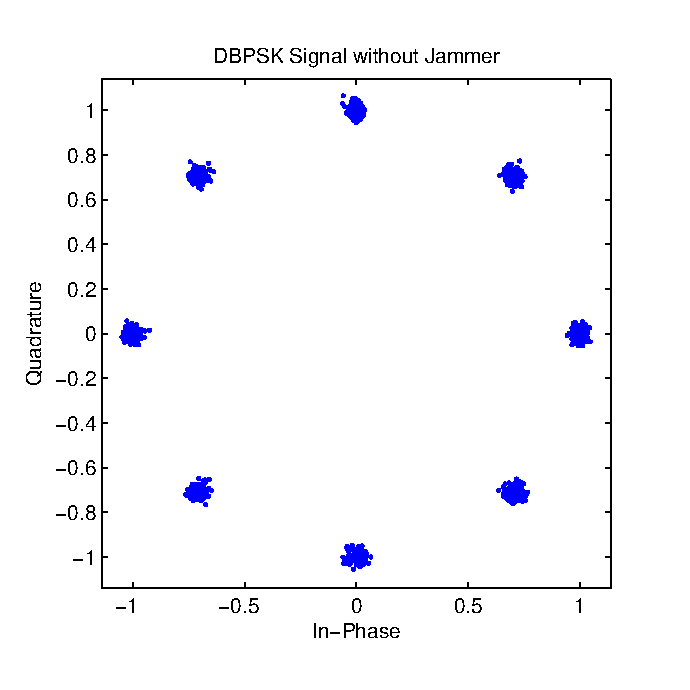
\includegraphics[width=\linewidth]{DBPSK_nojam.eps}
    \caption{DBPSK signal uncorrupted by jammer.  Clean clustering around the constellation points provides accurate symbol recovery.}
    \label{fig:chapter001_dist_001}
  \end{minipage}
  \hspace{0.5cm}
  \begin{minipage}[b]{0.5\linewidth}
    \centering
    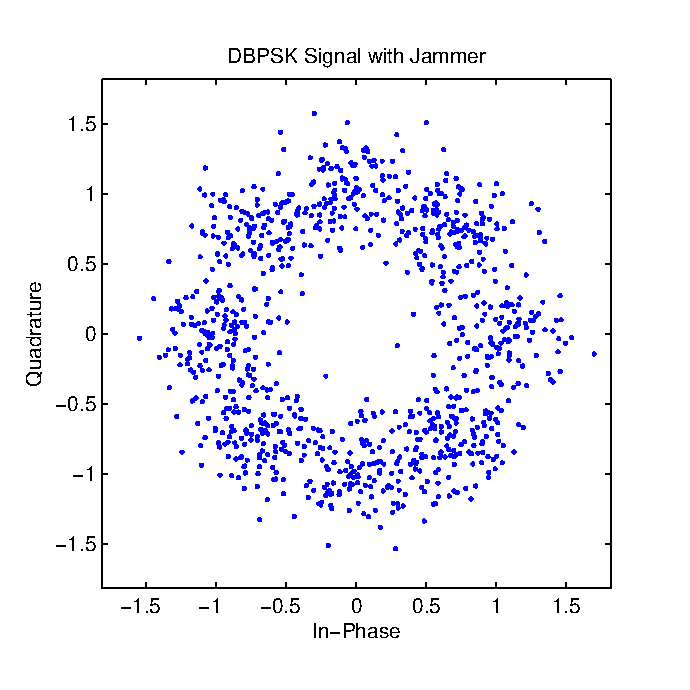
\includegraphics[width=\linewidth]{DBPSK_jam.eps}
    \caption{DBPSK signal corrupted by jammer.  The overlapping clustering around the constellation points provides difficult symbol recovery.}
    \label{fig:chapter001_reward_001}
  \end{minipage}
\end{figure}

\section{Anti-Jamming}

Anti-jamming has been considerably outlined in the Introduction chapter, therefore this section will examine more advanced narrowband and wideband techniques that involve filtering rather than avoidance.  All of these approaches have various monitary costs, constraints, and power limitations.  First, narrowband mitigation techniques will be considered.  These include adaptive filtering, time-frequency domain filtering, adaptive antennas and subspace processing.  By combining several of the listed techniques, wideband jammers can also be address, under certain conditions.  Table \ref{antitable} compares these techniques with various attributes.\\

\begin{table}[!ht]\label{antitable}
\centering
\caption{Comparision of Anti-Jamming Techniques}
\resizebox{\columnwidth}{!}{
    \begin{tabular}{|l|l|l|l|l|l|}
        \hline
        Technique                       & Cost & Size  & Flexibility                              & Complexity  \\ \hline
        Adaptive Filtering              & low  & small & ~                                        & ~           \\ 
        Time-Frequency Domain Filtering & ~    & ~     & ~                                        & ~           \\ 
        STFT                            & low  & small & Environment Specific                     & low         \\ 
        Filter Banks                    & low  & small & Environment Specific                     & low         \\ 
        Wavelet Transform               & low  & small & Environment Specific/Resolution Required & low         \\ 
        Subspace Processing             & low  & small & ~                                        & ~           \\ 
        Adaptive Antennas               & ~    & ~     & ~                                        & ~           \\ 
        Null Steering                   & high & large & ~                                        & high        \\ 
        Beam Forming                    & high & large & ~                                        & high        \\
        \hline
    \end{tabular}
}

\end{table}

Adaptive filtering is a well defined solution in jammer mitigation, but it is to date the most limited.  Most notably, the jammer must be a relatively narrowband and the period of the jammer must be relatively short.  An example of an adaptive filtering technique is a suppression filter.  Suppression filters assume statistically the signal is Gaussian, which results in the optimal filter being linear.  This filter essentially solves the Wiener equation for an optimal filter, but generally a Least Mean Square (LMS) implementation is used instead of just inversing the channel estimate \cite{11}. The technique of inverting the channel estimate or correlation matrix is traditionally called a zero forcing equalizer and is extremely unstable in the presence of small noise.\\

Next, time-frequency domain filtering attempts to represent the transform the received signal in such a way that it is possible to easily distinguish the jammer from the data signal.  A Short-Time Fourier Transform (STFT) can be used to accomplish this goal.  A STFT operates by sliding a window across a signal and taking the fast fourier transform (FFT) of that window. Reference \cite{12} uses the STFT to break a signal into its frequency components. From this information, with a narrowband jammer only a small number of frequency domain bins contain nearly all of the interferers.  Therefore these bins can be simply nulled and an inverse FFT can be applied to the signal to regain its time domain version.  This is very effective with the use of a spread spectrum signal with a narrowband jammer.\\

%\being{equation}
%
%\displaystyle\sum_{n=-\infinity}^{\infinity} n^{2}
%
%\end{equation}

Filter banks is a second methodology that can be used to reduce spectral leakage in the frequency domain, which is the primary drawback with the STFT approach.  One advantage of the filter banks approach is they do not inject interference when the jammer is not present, which is a common problem when the jammer turns on and off frequently.  Filter banks provide jammer suppression after their spectral decomposition stage, since at this point sub-band encoding can be accomplished this spectral modification simply nullifys the jammer \cite{13}.  A similar decomposition is the wavelet transform.  Unlike the STFT, the wavelet transform is much more flexible because the STFT has a fixed resolution for a given FFT size unlike the wavelet transform \cite{wavelet}.  Subspace processing which is a form of wavelet transform, is applied in this way.  The jammer subspace can be made orthogonal to the wanted signal subspace, nullifying the jammer's effects \cite{14}.\\

Besides these signal processing methods, physical techniques can also be use to do spatial filtering.  These techiques make use of several antennas, and as an assumption the number of interferers must be equal to or less than the number of antennas.  The first approach is called Null Steering.  Null Steering constantly computes the weights in order to minimize the received energy level. In effect, this technique attempts to steer the antenna away from the jammer.  The second approach is called Beamforming.  Beamforming tries to adjust the antenna in order to maximize the SNR. In effect, the antenna beam is steered in the direction of the desired signal.  It is of course, possible for the jammer's signal to be in the same direction as the signal source. Therefore the postcorrelation technique is used in order to obtain the SNR. However, prior knowledge of the signal direction and the host location is required \cite{kandangath}.  It is also important to note that larger the number of elements in the array itself, the closer the jammer can physically be located to the desired transmitter.\\


Historically, all of these approaches historically were applied to spread spectrum communication systems because narrowband jammers fundamentally are considerably easier to deal with in this setting.  They are more straightforward because the jammer effects only a fraction of the transmitter's transmission space; therefore, when wideband jammers exist many of these schemes fall apart.  Other avenues or scenarios must be considered in such situations to overcome this limitation.  Before a solution is chosen, additional signal processing and communication theory must be understood.  These topics will be examined in the following sections.\\



\section{Communication Systems}

Modern wireless digital communication systems are based on a rich tradition of analog experimentation and theory.  These signal technologies surround us constantly, such as cellphones, car radios, GPS, and more.  All these of these devices communicate over wireless links and are built upon the same building block of transmission and reception theory.  Many perspectives can be taken, but a more generic observation should be taken at the system level.  Depending on the level of sophistication these blocks can expand greatly, but still solve the same issue caused by the wireless transmission of digital access across their environment.  Such non-idealities such as frequency offsets, doppler effect, signal echoes, phase shifts, and others must be compensated for to successful receive uncorrupted information.\\ 

Let us examine the transmitter first since it is less complicated than the receiver.  The transmitter's primary goal is to send data in a resilient form, or structure, to create a more managable signal for the receiver.  This is accomplished in several steps, and the function, or purpose, of the overall system determines the sophistication of the design.  Figure \ref{fig:Transmitter_System_Diagram} outlines the major building blocks of the transmitter; consisting of the coder, pulse-shape filter, and frequency translator.  A filter is added after the coding block in some implementations to provide such effect as pre-distortion.\\

\begin{figure}[!ht]\label{fig:Transmitter_System_Diagram}
\centering
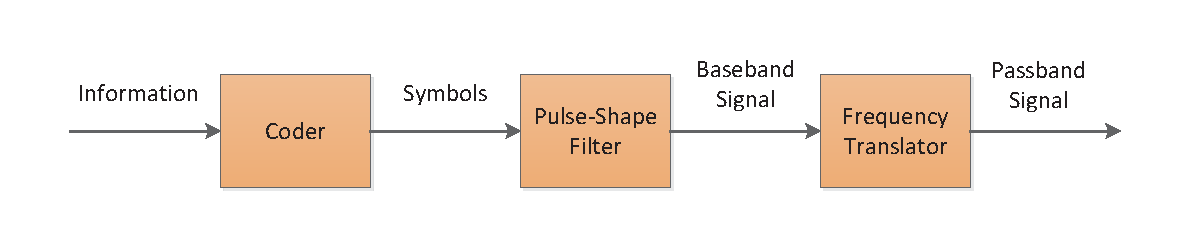
\includegraphics[scale=0.8]{Transmitter.eps}
\caption{Basic transmitter outline, converting information or data to a easily recoverable signal by the receiver.}
\end{figure}

The transmitter's sole purpose is the send data that is convenient for the receiver to understand, and allow others to use the transmission medium as well.  The coding phase of the transmitter can have many features and purposes, but simply it will encode data into a symbol with a form of redundancy or scheme that will help the receiver reconstructed the information more easily.  Next the pulse-shape filter is used to help separate data and help maximize the SNR at the receiver.  This filtering can be done with an assortment of filter shapes, but the most popular is the raised square-root cosine filter.  After pulse-shaping, the signal is translated into frequency information and unconverted to a high RF with a carrier signal.  The translation is done with a modulation scheme such a binary phase-shift keying (BPSK) or pulse amplitude modulation (PAM).  The is up-converted by mixing the signal with a sinusoid, seen by Equation \eqref{mixing}.

\begin{equation}[!ht]\label{mixing}
cos(x)cos(y)=\frac{(cos(x+y)+cos(x-y))}{2}
\end{equation}

This done because low-frequency signals such as speech, music, or digital data can be much more efficiently transmitted at higher frequencies \cite{9}.\\

Now let us discuss the receiver.  At the system level, a modern digital receiver can be broken down into a small set of distinct categories or operations: carrier synchronization, timing synchronization, equalization, and frame synchronization, as outlined in Figure \ref{Receiver_Blocks}.  These sections work together in series to provide smooth transmission of data, and many techniques exist within theses categories to accomplish its goal.  In most communication systems, after the radio frequency (RF) front-end, the first operation done on the received signal is frequency compensation and down conversion.  This compensation needs to accomplished because non-idealities and differences exist between the transmitter's and receiver's oscillator.  Therefore this is continually compensated for and corrected.  Carrier recovery can be accomplished using several methods that include but are not limited to: squared difference loops, phase-locked loops, costas loops, and decision-directed phase tracking \cite{9}.\\

\begin{figure}[!ht]\label{Receiver_Blocks}
\centering
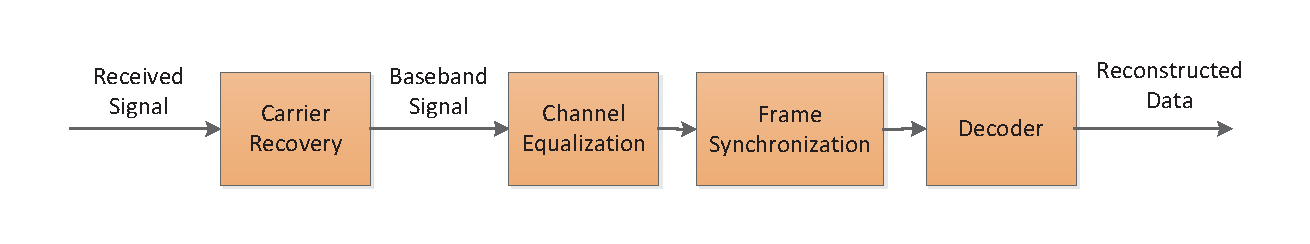
\includegraphics[scale=0.7]{Receiver.eps}
\caption{Basic wireless receiver outline, with four primary blocks.  All designed to remove corruption caused by the wireless environment and translate transmitted signals back to desired data.}
\end{figure}

After carrier recovery, the signal is pulse-shaped with the same filter shape used at the transmitter.  This technique will help to maximize the SNR of the signal.  Then the signal must be corrected again for timing.  The purpose of timing recovery is to choose the instants at which to sample the incoming signal.  This is generally done through a interpolation mechanism of the transmitted signal.  Since at the transmitter the signal is upsampled to symbols, a single data point or bit is represented by several received data points.  Therefore these points can be interpolated together for a more accurate estimate of the original data.  Timing recovery also can be done with one of several methods including: output power maximization, Mueller-Muller method, or decision-directed.  Generally, they utilize their own interpolation algorithm, such as sinc-interpolation \cite{9}.\\

After this point the receiver designs can vary greatly, as the design in this thesis will present, because this is where most of the digital signal processing (DSP) will take place.  This section, call Equalization, is responsible to correcting any effect the channel has on the signal. This includes multi-path, noise, 	and other distortions that cause inter-symbol interference (ISI).  Equalizer implementations are designed to compensate for types of disturbances that occur using certain systems.  The equalizer stage is most often coupled with the frame synchronization stage such that the equalizer itself can adapt to changing conditions.  This is known as soft decision making.  Equalizer techniques include but are not limited to: LMS , decision-directed, dispersion-minimizing \cite{9}, Viterbi \cite{viterbi}, blind, and turbo equalizers \cite{turbo}.\\  

\subsection{Equalization}

Equalizers can be considered the most complicated design of an entire communication system since they combat a series of distortions.  The primary result of these distortions is called inter-symbol interference (ISI).  ISI simply means that symbols interact with one another in the channel space and cannot be considered independent from one another.  Since this interference is generally considered a frequency selective disruption or dispersion a filter needs to be employed to reverse such effects.  This filter must be adaptable because the channel distortion cannot be know prior to transmission.\\  

As listed in the previous section, many equalizers exists and operate under specific conditions.  Here several linear equalizers will be discussed in detail including maximum-likelihood sequence detection, adaptively trained equalizer, and decision-directed linear equalization.  The goal of all of these equalizers is to find a finite impulse response (FIR) filter that when convolved with the received signal produces the original transmitted data \( \boldsymbol{\hat{X}}=\bf{Y} * \bf{G} \).  Figure \ref{FIR_filter} outlines a typical FIR structure for which the equalizer will create the appropriate coefficients \(b_{0},b_{1},..., b_{n} \).  These equalizers also examine the condition of an additive white Gaussian noise (AWGN) channel, and uncorrelated or independent interferers.\\

\begin{figure}[!ht]\label{FIR_filter}
\centering
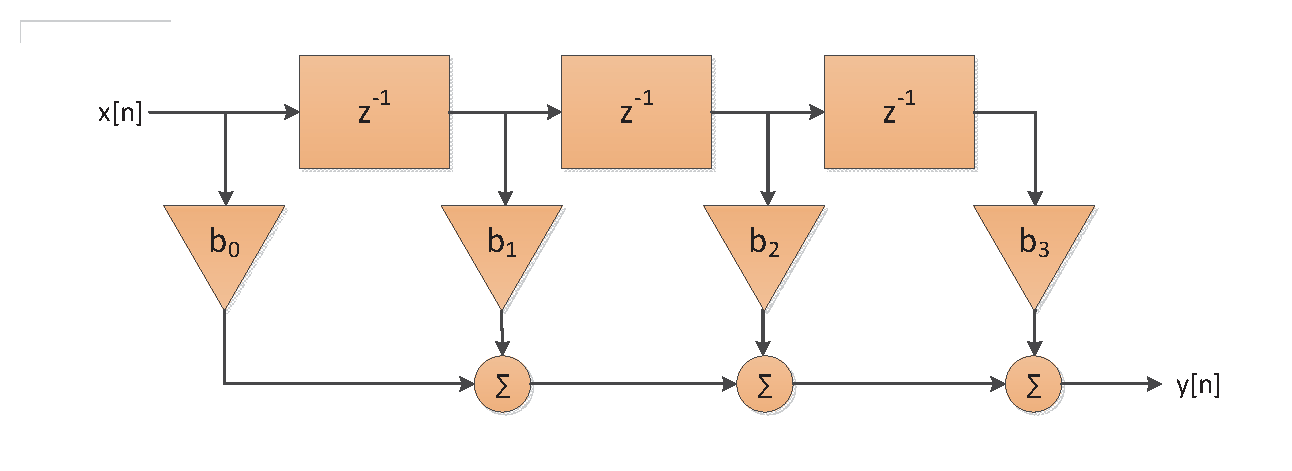
\includegraphics[scale=0.7]{FIR_filter.eps}
\caption{FIR Filter Structure}
\end{figure}

The Zero Forcing Equalizer (ZFE) uses peak distortion criteria to determine equalizer coefficients.  The ZFE produces zero ISI at its output.  If \(H_{c}(f)\) is assumed to be the effects of the channel, the ideal equalizer would be \( H_{eq}(f)=\frac{1}{H_{c}(f)}\).  This can also be consider the inverse of the channel.  The filter coefficients are modeled as weighted pulses convolved with the channel, which can be expressed as Equation \eqref{weighted}.  Here \(b\) represents the weighted filter taps, \(p_{r}\) represents the input signal and \(p_{eq}\) represents the output of the filter.

\begin{equation}\label{weighted}
p_{eq}(t) = \displaystyle\sum_{k=-M}^{M} b_{k}p_{r}(t-kT)
\end{equation}

Unfortunately, the ZFE has a large disadvantage; it cannot compensate for small amounts of noise.  Technically, the ZFE will amplify all noise of the received signal, and if any elements of the channel matrix are considerably small, then the equalizer becomes unstable. Therefore this is generally considered a more theoretical or elementary equalizer formulation.  To overcome this problem the zero ISI condition must be relaxed allowing for noise which if small can easily be overcome by such operations as quantization or decision making.  The Linear Minimum Mean Squared Error Filter (LMMSE) takes this relaxation into account \cite{spinger}.\\ 

The LMMSE assumes that the symbols are uncorrelated with one another and uncorrelated from the noise in the channel.  This approach tries to minimize the mean square error, a common measure of estimator performance.  The estimator is defined as \(\hat{x}_{MMSE}(y)=E{x|y}\), where we are given the received signal \(y\) and must guess or estimate \(x\), which was transmitted originally.  If \(x\) and \(y\) are jointly Gaussian, then the LMMSE will be linear.  This function or equalizer design minimizes the mean square error.  To simplify further an extension to random vectors can be examined.  An estimate can be made for the original vector \(x\) represented by \(\hat{x}\), resulting in the linear equation \(\hat{x}=ay+b\).  \(a\) and \(b\) represent the coefficients to be selected for the estimator.  The LMMSE will minimize the mean square error shown in Equation \ref{mse}:

\begin{equation}\label{mse}
 MSE = \|x-\hat{x}\|^{2}
\end{equation}

Besides these linear equalizers outlined, an adaptive approach can also be considered.  The Least Mean Squares (LMS) or Gradient Descent algorithm utilizes a traditional technique for minimizing the error in a signal.  This method is historically known as the "Method of Steepest Decent" or a very closely related algorithm called "Newton's Method". By calculating the error of each received symbol, this can be fed back into the system for future symbols.  This error will shape the equalizer's filter coefficents to match the inverse of the channel.  The equations \ref{lms_eq}, \ref{lms_eq2}, and \ref{lms_eq3} outline the LMS algorithm.

\begin{equation}\label{lms_eq}
y[n]=w[n]^{H}u[n]\\
\end{equation}

\begin{equation}\label{lms_eq2}
e[n]=d_{n}-y[n]\\
\end{equation}

\begin{equation}\label{lms_eq3}
w[n+1]=w[n]+\mu u[n]e^{*}[n]\\ 
\end{equation}

In these equations: \(w\) represents the adaptive filter coefficients, \(u\) the input signal, and \(d\) the known signal.  \(\mu\) acts as the algorithm's step-size determining how quickly it will converge.  It must also be considered that the larger the step-size the higher the probability it may become unstable.  As long as the channel's effects are slow changing, this equalizer can easily maintain up to date estimates while corrupting as little of the data as possible.\\  

All of the methods proposed so far require \textit{known} data (\(d_{n}\) in Equation (\ref{lms_eq2}) to correct against.  This data is called training data and generally comes in the form of a preamble in a frame.  The preamble is added to the beginning of each frame so the equalizer can learn from the effects on that specific data.  The preamble is the same for all frames and is always used so the equalizer will always be learning.  However, what happens when data is unknown in the frame, such as the payload portion of the frame.  This is where blind equalization is employed.\\

Several blind equalizers exist but an extension of the LMS equalizer for blind situations will be examined here called the decision-directed equalizers \cite{9}.  For a blind equalizer to operate an error generation mechanism must be evaluated, but since the data symbols are unknown, a decision device must be used in place.  This decision device is a quantization method and the error is generated from this quantization.  This error generation is extrapolated from expression: 
\(e = \frac{1}{2}(sgn(y[k]-y[k])^{2}\)
Where the \(sgn\) function returns 1 for positive numbers and -1 for negative numbers.  This expression is quite similar to the original LMS implementation except instead of a known symbol the data is quantized using the sign function.  This type of quantization using the sign function is only applicable with binary modulation schemes such as BPSK.  This equalizer method is usually combined with a training equalizer method in practice, since if a nearly closed eye is observed, when using an eye diagram, this equalizer cannot open it by itself.  An example of such an eye diagram is shown in Figure \ref{eye_closed}, and clean/open eye diagram can be seen in Figure \ref{eye_clean}.\\

\begin{figure}\label{eye_clean}
\centering
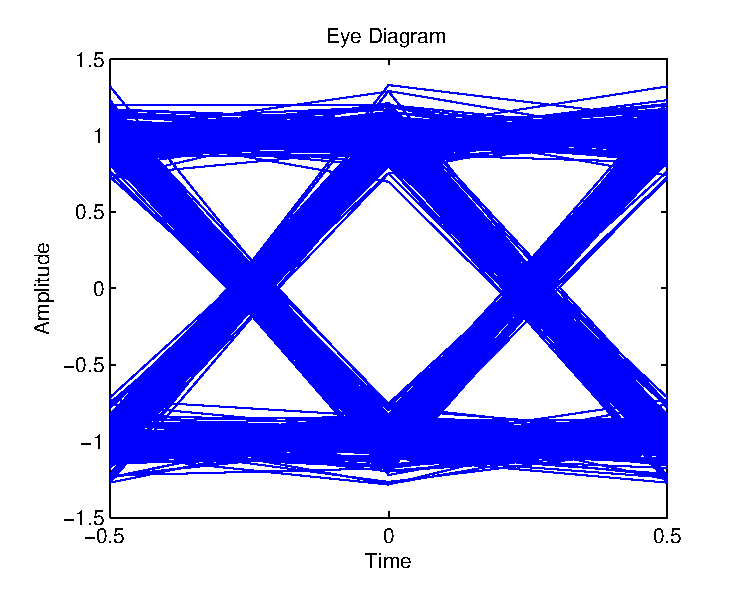
\includegraphics[scale=0.8]{eye_clean.eps}
\caption{Adequate timing recovery produces open eye, which clearly defines the received symbols in time.}
\end{figure}

\begin{figure}\label{eye_closed}
\centering
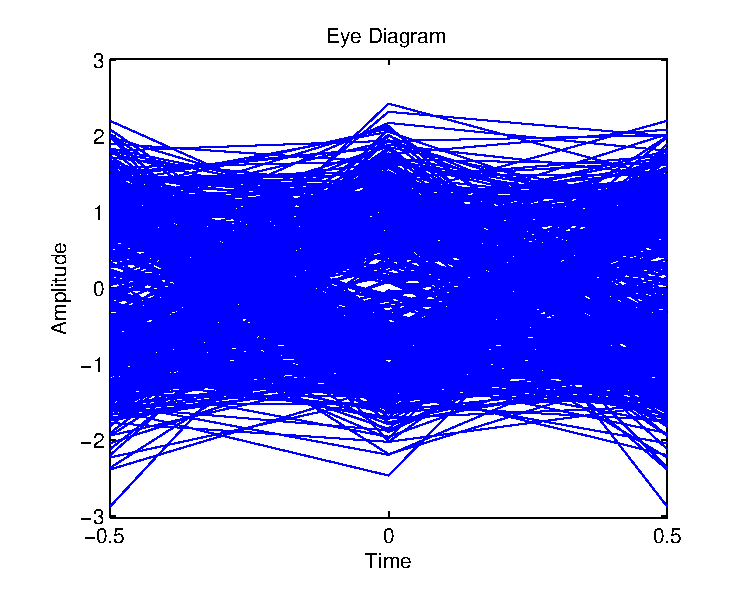
\includegraphics[scale=0.8]{eye_closed.eps}
\caption{Poor timing recovery produces a closed eye, identifying that the signal cannot be recovered unless corrective measures applied.}
\end{figure}

In this section, we have examined several equalizer techniques while outlining their advantages and disadvantages.  Most techniques require some training mechanisms to operate under heavy channel distortion, and blind techniques such as decision-directed equalization will fail under these conditions.  Unfortunately, such training data can take considerable resources, and lower overall data throughput.  In practice as much as 20\% of frame information is training.  Therefore other techniques must be considered to help overcome this obstacle.\\


\subsection{Superimposed Training Equalization}

As mentioned in the previous section, many implementations exist for equalizer designs, but this thesis will examine the effectiveness of superimposed training symbols in frequency selective channels.  In traditional equalizers, channel estimation is achieved through the use of training data or pilot symbols.  These symbols are both known to the transmitter and receiver, providing the basis for an estimate.  In these equalizers all training symbols are placed at the start of a frame, with \cite{16} showing that under high SNR training-based schemes are capable of capturing most of the channel capacity, while under low SNR they are highly suboptimal.  Superimposed equalizers try to overcome this problem along with others to provide more optimal estimates.  Superimposed equalizers physically add training symbols to the data stream instead of concatenating symbols, saving valuable bandwidth \cite{16}.  To accommodate such pilots, energy must be shared among the data and hidden pilots \cite{Ghogho}.  Reference \cite{19} shows that for a transmitter of fixed power, with an additive pilot sequence, the decrease in data signal power is equal to: \[ K_{loss}=\frac{E[\|s(k)\|^{2}}{E[\|s(k)\|^{2}]+E[\|u(k)\|^{2}]}\] equivalent to \(10logK_{loss}dB\) in signal to noise ratio (SNR).  With \(s(k)\) representing the source signal, and \(u(k)\) representing the received signal.  Other disadvantages include an increased signal envelope fluctuation that can be undesirable in nonlinear transmit power amplifiers \cite{17}.\\  

At the receiver, channel estimation can be done using several techniques in both the frequency and time domain.  Reference \cite{17} examines a time domain approach for synchronized averaging of the received signal.  It is important to note that this synchronization is not related to transmitter and receiver synchronization.  References \cite{17} and \cite{18} both assume that the signal \( \bf{x}(n)\) and noise \( \bf{v}(n) \) have zero mean and \(E[m_{x}(n)] = \bf{d}(n) = \bf{p}(n) \ast \bf{h}(n)\).  Therefore, since \(\bf{p}(n) \) is the known superimposed periodic pilot sequence, \(\bf{h}(n)\) can be determined.  Note that \(\bf{h}(n)\) is generally considered frequency selective, and such channels can be quite difficult to deal with especially with multi-path.  Multi-path interference is a distortion caused when copies of the original signal arrive at the receiver delayed on top of the originally received non-delayed signal.  This delayed signals essentially take other paths to the receiver, and this interference's manifestation is commonly called \textit{ghosting} in such applications as television broadcasts \cite{ghost}.\\

Superimposed equalizers are able to better compensate for large multi-path channels because they can spread their training symbols throughout the signal itself.  This spreading not only provides a spreading in time but also in other dimensions such a frequency.  Therefore, if the training symbols are chosen correctly and placed correctly, they can then be spread across the frequency spectrum efficiently and capture its selectivity.  Before the pilots can be examined, the channel must be defined.  The channel is of block length \(N\), and the channel is also time invariant across single blocks, but variable across blocks.  The memory of this channel is of maximum length \(L-1\), and the impulse response of the channel is defined as \(\textbf{h}=[h_{0},...,h_{L-1}]^{T}\).  Since there are \(N\) blocks in the channel, the channel matrix \(H\) is modeled as an \(N x N\) circulant matrix, with the received signal as expressed as:

\begin{equation}
\textbf{x}=\textbf{H}\textbf{s}+\textbf{v}
\end{equation}

Here, \(\textbf{v}\) is assumed to be zero mean white noise.  The vector \(\textbf{s}\) is a combination of known training symbols and unknown data.  The optimal placement for such training is where the channel undergoes non-ergodic fading considered here \cite{20}.  Reference \cite{16} continues on to say that optimally, assuming symbols are placed in clusters of length \(\alpha \ge 2L+1\), this scheme is quasi-periodic.  The variable \(\alpha\) represents the cluster size in this scenario.  It is also important to note that this placement makes sure that the training is always orthogonal.\\

Another effect that must be considered is how these training symbols interfere with the data itself, and is the training symbols dependent on the data or even the modulation scheme.  Reference \cite{Ghogho} examines this aspect and proposes solutions that provides a data independence condition.  As explained previously, since the training data is periodic it can be placed in equispaced frequency bins, while data is spread across all frequency bins.   Therefore, the pilot must be designed to distort the data vector of the discrete Fourier transform to zero.  In the superimposed training data case, this is done by using the cyclic mean of the data.  Therefore, all that needs to be done is the removal of the cyclic mean \(\textbf{e}=\textbf{Jw}\).  Note that \(\textbf{J}\) is the Kronecker product of an identity matrix and the fractionally spaced locations of the pilot tones.  Therefore, at the pilot frequency only the training symbols are visible for the channel estimation.  Formally here is the transmitted, or precoded, result including pilots and data: \( \textbf{s}= (I-\textbf{J})\textbf{w}+\textbf{c}  \).\\


In summary, research on superimposed training focuses primarily on the training symbol generation for a certain type of communication systems design from single transmission to multiple-input multiple-output (MIMO).  Unfortunately, little to no physical implementations exists for such systems.  This is true because of the synchronization issue that exists when using superimposed training symbols.  Since they are directly placed with transmission data it can be difficult to determine their locations in a sequence blindly, which is done in real world systems.  This problem must be considered when physical implementations are proposed.\\

\section{Spectral Subtraction}

Now that methods of reconstructing information distorted by the channel itself has been discussed, we can now focus on spectral removal of known signals without demodulation.  Such a technique is needed to improve the effectiveness of equalization operations done downstream, while limiting corruption to the desired signals themselves.  In this thesis a new application for a relatively standard technique was examined, called Spectral Subtraction (SS).  The SS technique was first published in 1979 by Steven Boll \cite{boll}. SS is formally used to reduce ambient noise in audible sources, improving the overall quality and intelligibility of digitized speech.  It is a dominant speech processing algorithm and many extensions including \cite{SSEXAMPLE}, \cite{SSEXAMPLE2}, and \cite{SSEXAMPLE3}.  Due to the large amount of literature and investigation into the SS process it was assumed to be a solid option for removing unwanted signals in the spectrum.\\

SS primarily was designed for audio signal processing, small bandwidth signals roughly from 20Hz to 20,000Hz.  Many forms of SS exist, but the approach examined here is Magnitude Spectral Subtraction (MSS).  It works by first generating an estimate of the noise in the signal itself, which is usually attained at the first first few seconds of the signal itself.  This noise is then subtracted, as the name suggests, from the rest of the signal.  Mathematically, let us explain this further.  The received signal is assumed to be a combination of two signals, the transmitted and the noise itself \(y(t) = x(t) + n(t)\).  Next the power spectral densities (PSD) are calculated for these components:

\[ E\{|Y(e^{jw}|^{2}\}= E\{|X(e^{jw}|^{2}\} + E\{|N(e^{jw}|^{2}\} + 2E\{|X(e^{jw}|^{2}\}\{|N(e^{jw}|^{2}\}\]
\[ E\{|Y(e^{jw}|^{2}\}= E\{|X(e^{jw}|\} + E\{|N(e^{jw}|\}  \]

Here \(Y(e^{jw})\), \(X(e^{jw})\), and \(N(e^{jw})\) represent the frequency domain transform of the given signal, also \(x\) and \(n\) are uncorrelated.  Since at points when the desired signal is not present in the spectrum, a silent period, the measurement for \(N\) is taken and then subtracted from the entire received signal \(E\{|X(e^{jw}|\}= E\{|Y(e^{jw}|\} - E\{|N(e^{jw}|\}\).  The is noise is assumed to be quite stationary during the signal period.  Therefore, the original estimate \(\hat{N}\) can be quite accurate.\\

\subsection{Residual Noise}

As a result of the changes over time in the noise spectrum (whether power or magnitude) around its expected value, there is always some difference between the actual noise and its mean value. Hence, some of the noise remains in the spectrum in the case that the value of noise is greater than its mean and some of the speech spectrum also is removed in the case that the estimate of noise to be greater than the actual value of noise. The latter produces negative values in the spectrum. These negative values are prevented or set to a floor (sometimes zero) using different techniques. The overall effect puts noise in the output signal known as residual. The narrow band relatively long-lived portion of residual noise is sometimes referred to as musical noise \cite{mnoise}.

A close examination of musical noise, shows that peaks and valleys exist in the short term power spectrum of white noise.  These frequency locations for one frame are random and they vary randomly in frequency and amplitude from frame to frame. When a smoothed estimate of the noise spectrum is subtracted from the actual noise spectrum, all spectral peaks are shifted down while the valleys are set to zero. Therefore, after this subtraction sharp peaks remain in the noise spectrum and pre-existing ones can be sharpened. The wide peaks are generally estimated as time varying broadband noise. The narrower peaks, which are relatively large spectral distances because of the deep valleys that define them, are perceived as time varying tones which are generally referred to as musical noise \cite{berouti}.

Therefore, \cite{boll} continues by introducing a ``smoothing'' technique before the signal is convert back into the frequency domain.  Two additional parameters are introduced: The parameter \( \alpha \) the over-subtraction coefficient, and \(\beta\) the noise floor lower bound.  \(\alpha\) is used to provide a more aggressive subtraction to the signal, attacking high peaks which are generally a result of high noise and an inaccurate initial estimate.  The second parameter \(\beta\) is used to fill in the valleys of the signal.  Since if an over-subtraction takes too much signal it can cause valleys in the spectrum below or above the zero threshold.  This value is used to simply quantize values within its +/- limits.  As a result these operations together produce a smoother signal removing much of the residual noise from just a plain subtraction.  Reference \cite{boll} provides several results examining the benefits of such a technique.\\  


\section{Software Defined Radio}

Now that the signal processing techniques have been discussed, a platform for implementation is needed.  The alley chosen for this thesis is to utilize a new hardware frontier called Software-Defined Radio, which will be discussed in this section.\\

For the past two decades there has been a paradigm shift is the definition of a radio device.  The conversation has to do with the question of where hardware ends and where software begins.  The term Software Defined Radio, coined by Dr. J. Mitola III,  defined as a set of digital signal processing (DSP) primitives, a meta-level system for combining the primitives into communication system functions (transmitter, channel model, receiver, etc.), and a set of target processors on which the software radio is hosted for real-time communications \cite{21}.  Dr. Mitola understood how software provided the flexibility that hardware never could, and as time made it more mailable SDR would become dominant.\\

SDRs can be flexible enough to avoid the ``limited spectrum'' assumptions of designers of previous kinds of radios, in one or more ways including: Ultrawideband transceivers, cognitive radio, dynamic mesh networks, software-defined antenna arrays among others \cite{22}.  One of the first SDR implementations was a project called ``SpeakEasy''.  The original purpose of SpeakEasy was to use programmable processing to emulate more than ten existing military radios, operating in frequency bands between 2 MHz and 2 GHz \cite{23}.  Therefore with this single radio, the operator could talk to ten radios operating under ten different standards.  As simple enough idea, but unfortunately the implementation left much to be desired.  For example, physically the device encapsulated the entire back of a common pickup truck \cite{23}.  This might be great for a ground station that does not move, but for a mobile unit this was highly impractical.  Secondly, in 1992 field programmable gate arrays (FPGA) required significant time, comparatively to re-flash or change their operational parameters.  Again, this also limited SpeakEasy's flexibility.\\

\begin{figure}\label{sdr_overview}
\centering
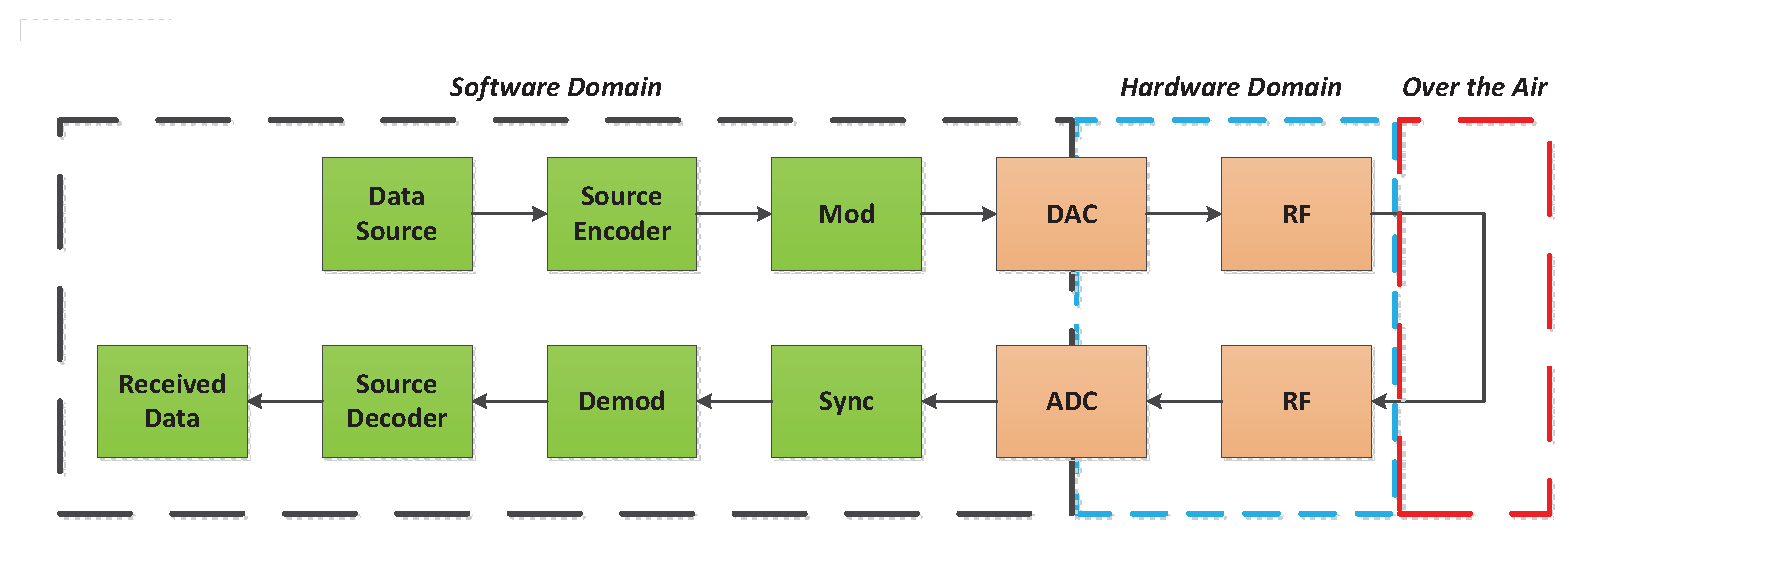
\includegraphics[scale=0.8]{sdr_overview.eps}
\caption{Software Defined Radio push all the adaptive elements and data manipulation operation into software.  The goal of SDR is to provide or define all of the radio operation in software.}
\end{figure}

Today, the main target implementations are within cellular base stations and military applications such as the JTRS project.  The JTRS or Joint Tactical Radio System, was a program of the US military to produce radios that provide flexible and inter-operable communications \cite{JTRS}. Examples of radio terminals that require support include hand-held, vehicular, airborne and dismounted radios, as well as base-stations\cite{24}.  Again, this project still has limited results and many setbacks have occurred.  Commercially, from a wide spread penetration standpoint, SDR is still many years away due to the size and cost of current devices.  The two barriers to this are speed and size.  To provide enough data throughput, modern SDRs need to quite large physically, which is a serious drawback in many applications.   Aside from these limitations, SDRs provide excellent flexibility especially in a laboratory and proof of concept environment.  Rapid prototyping is an obvious place where such radios shine, allowing massive changes without hardware modification.  To support this flexibility several software packages have been constructed around the SDR concept, allowing for aggressive prototyping.  The two examples discussed here were selected because of operability with the selected hardware, which will be discussed future in chapter 3.\\

\subsection{GNU Radio}

The first software package to be discussed by this thesis is GNU Radio.  GNU Radio provides the reconfigurable signal processing blocks that are necessary for software defined radios. GNU Radio is an open source project allowing for SDR developers to develop unique signal processing blocks and SDR systems.  GNU Radio was started in 2001, originally forked from the SpectrumWare project developed at the Massachusetts Institute of Technology \cite{spectrumware}.  Since 2001, the code base has undergone massive changes, containing almost no code from the original SpectrumWare project.  Physically the code consist of three languages Python, C++, and SWIG.  Python provides the overarching control of the system or program, while C++ provides the actual signal processing blocks and mathematics.  SWIG is a wrapper for C++ which allows Python to dynamically wrap around C++ and control or compile with it.  A diagram below better illustrates this architecture.  It is also important to mention that there as significant paradigm shifts in the community, pushing more and more code to Python rather than C++, due to its easier programming syntax and structure.\\

\begin{figure}\label{gnr_struct}
\centering
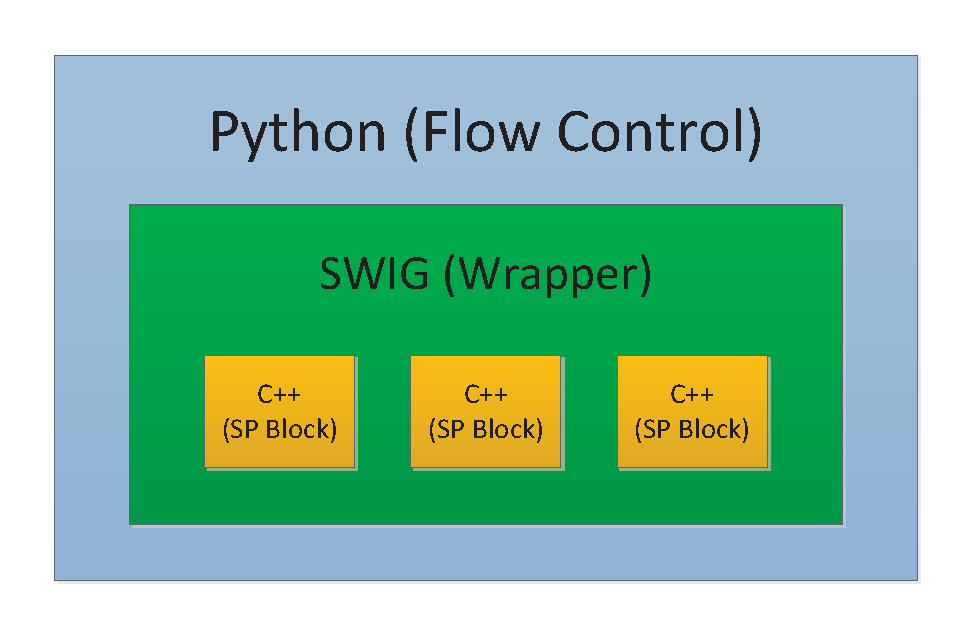
\includegraphics[scale=0.8]{gnr_outline.eps}
\caption{GNU Radio code structure based on signal processing C++ blocks and controlling, through SWIG, Python layers.}
\end{figure}

GNU Radio provides a very structured framework of flow design.  Data processing segments are extremely self contained to minimize error propagation during system debugging.  Since the software is open-source full access to all code is provide, giving low-level access to all operation within GNU Radio.  Much of the actions have been abstracted to limited the knowledge of the lower layers, but if specific actions are required for an application.  Then serious depth or knowledge is needed about the overall project's structure, which is quite overloading.\\

\subsection{MATLAB}

MATLAB is an extremely well known engineering, mathematical, biological, and financial software suite.  MATLAB provide massive data leverage and advanced communication system models and algorithm for significant data processing.  Since 2007, they have also provided hardware compliance with specific SDR platforms through their Simulink platform, and more recently within MATLAB itself \cite{matlabsdru}.  This thesis primarily utilizes the signal processing and communication system aspects of MATLAB, since MATLAB cannot fully utilize all aspects of the chosen hardware.  It is important to note under alternate constraints, MATLAB can provide adequate performance directly interfacing with hardware, especially when accessing its targeting features seen here \cite{matlabtargeting}.  Figure \ref{sdru_example} shows an example of a common MATLAB SDR model through Simulink.\\

\begin{figure}[!ht]\label{sdru_example}
\centering
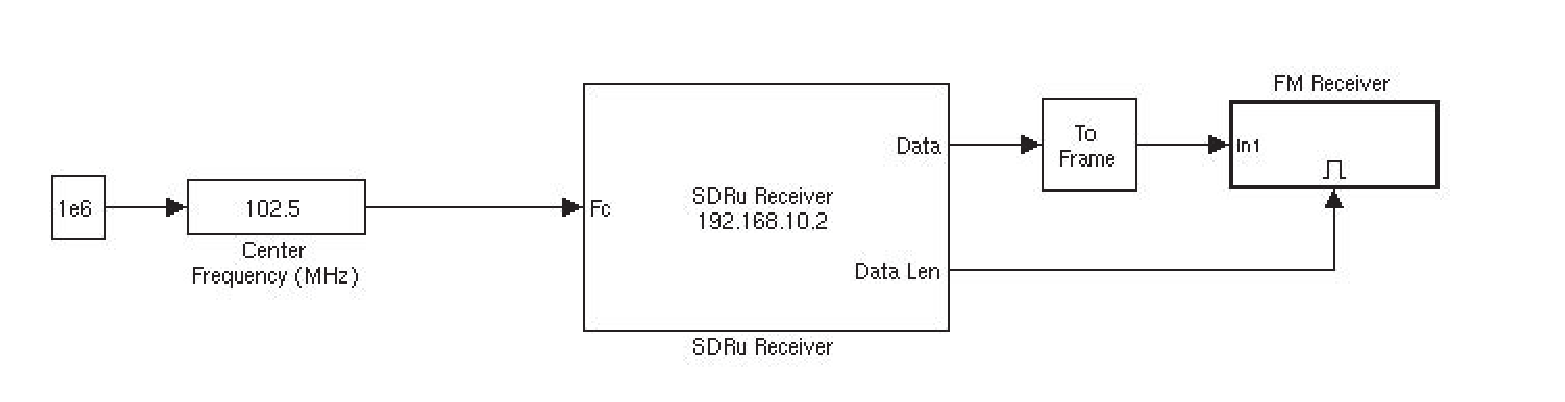
\includegraphics[scale=0.5]{sdru_example.eps}
\caption{Sample SDRU MATLAB model created in Simulink.  This model has the ability to demodulate and play FM radio stations when using a USRP device.}
\end{figure}

MATLAB provides allow connection to a USRP device through MATLAB directly of with Simulink.  The device simply acts as a real-time data source complementing their signal processing and communications toolboxes very well.  Rather than full implementations like GNUR Radio, MATLAB focuses on signal analysis rather than real-time performance.  The primary limitation is the single threaded nature of MATLAB and Simulink, which is slowly being improved upon for the SDR application.\\

\subsection{Reference Comparison}

It is important to compare GNU Radio and MATLAB, from a user's perspective they perform quite differently.  Firstly GNU Radio, is extremely fast, will the ability of sustaining the maximum throughput of the selected hardware.  GNU Radio is also multi-threaded, and while maintaining high throughput and complete background tasks on multi-core machines quite easily.  This performance has a cost, comparatively GNU Radio has an extremely learning curve and debugging can be challenging.  However if you need the performance, GNU Radio is your option, providing significantly more advanced hardware support in SDR implementations.  If data analysis is more heavily desired MATLAB is the obvious choice.  MATLAB provides easy and advanced data visualization functionality, and built in tools for analysis.  Since MATLAB does not compile itself normally, it can be much easier to debug and solve problems.  MATLAB's syntax provide similar data manipulation, especially in communication system primitives.  Therefore, it can be a rather simple choice, speed or ease of use.\\ 

\section{Summary}

This chapter outlined and examined the topics of jamming and anti-jamming techniques, and provided a foundation in communication system theory and advanced equalizer design.  Secondly it setup an understanding of Software-Defined Radio, the power of such an architecture, and examples of implementations and existing software for future designs.  Next, this thesis will consider a new anti-jamming technique and design an implementation of such a system.  After the implementation is investigated, the result of specific experiments on such an implementation will be analyzed.\\

%\chapter{Required Background Knowledge}
\label{ch:background}

This chapter provides the background information needed to understand the chapters that follow.  It examines the basic outline of a communication system and how non-idealities are compensated for, with the addition of multiple input multiple output (MIMO) systems and a unique filtering technique called spectral subtraction.   Secondly, this chapter investigates common jammer scenarios and anti-jamming solutions.  Finally, it outlines the necessary hardware and software tools used in the implementation chapter.

\section{Jamming}

In 1899 Guglielmo Marconi successfully transmitted radio messages across the English Channel, and nine months later Alexander Bell was discussing how this could be jammed during wartime \cite{10}. Bell stated that such a wireless system can be easily disrupted with simple electromagnetic distrubances:  ``It's as easy as cutting the wires'' \cite{10}.  In the early days of wireless communication, such systems were very fragile but today they have become substantially more resilient. In its simpliest form, radio jamming is the transmission of electromagnetic signals that interfere with communications by decreasing the signal to noise ratio (SNR) between the transmitter and receiver.  This jamming can be either deliberate or unintentional, and can either entirely disable the communication link or limit its capacity.  , a common example of unintentional jamming is microwave ovens which operate at a wavelength of 122 millimetres which translates to 2.45GHz from this equation: \(\lambda=\frac{v}{f}\), with \(lambda\) representing the wavelength, \(v\) the velocity and \(f\) the frequency. This band directly interferes with channels defined under the IEEE 802.11 standard, also known as Wi-Fi \cite{ieee80211}.  Deliberate jamming on the otherhand, is generally more saphisticated and takes many different forms.\\

Intentional communications jamming is usually aimed at radio signals in a combat setting, where consequences are insigificant or out of the relm of the law. In the most rudimentary designs, a jammer will simply tune their own frequency to that of their opponent and with a similar moduation scheme (and significant power) disrupt the enemies transmissions.  The most common types of this form of signal jamming are: random pulses, stepped tones, warbler, tones, rotary, pulses, sparks, recorded sounds, gulls, sweep-through, and random noise \cite{sterling}.  These methods obviously (or subtly) disrupt transmissions by inserting electronmagnetic energy into the transmission space of the receiver.  In more technical terms, the jammer is producing randomly chosen data that is non-orthogonal to the data which the friendly transmitter is producing.  Since this jammer's data is pseudo-random when his transmissions are added to the `oponent's' signal, the result appears to be random as well.  Therefore, the signal is unrecoverable.  As mentioned above, the jammer must produce signals that are non-orthogonal to the enemy of his jamming will have no effect.  An example below shows random noise at a significant noise level is added to a previously destinquishable signal.\\

\begin{figure}[!ht]
  \begin{minipage}[b]{0.5\linewidth}
    \centering
    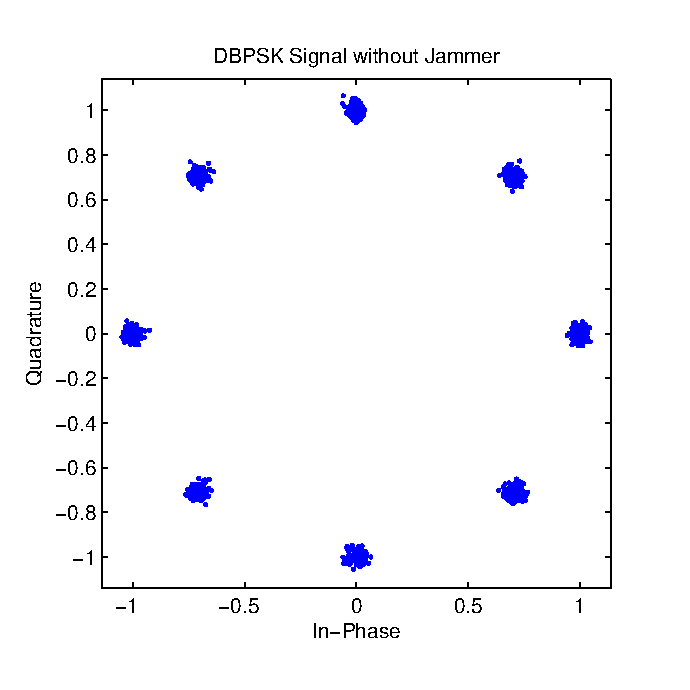
\includegraphics[width=\linewidth]{DBPSK_nojam.eps}
    \caption{DBPSK signal uncorrupted by jammer.  Clean clustering around the constellation points provides accurate symbol recovery.}
    \label{fig:chapter001_dist_001}
  \end{minipage}
  \hspace{0.5cm}
  \begin{minipage}[b]{0.5\linewidth}
    \centering
    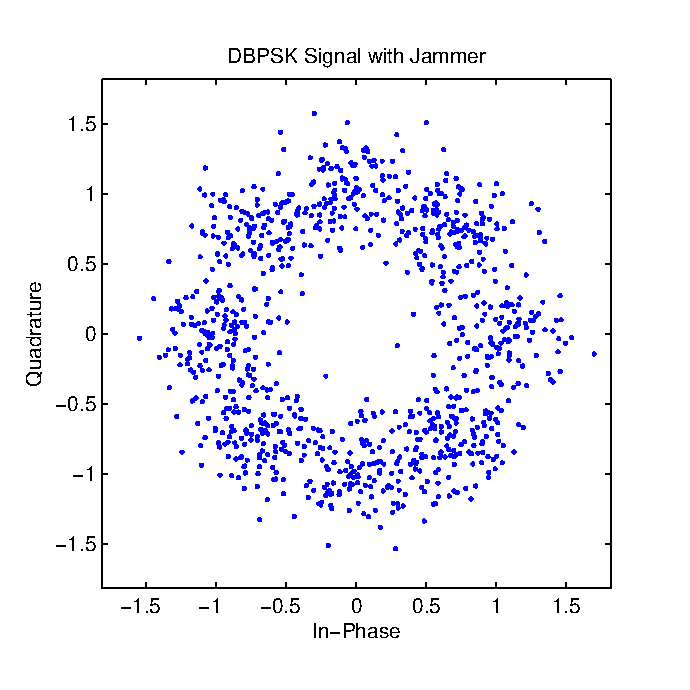
\includegraphics[width=\linewidth]{DBPSK_jam.eps}
    \caption{DBPSK signal corrupted by jammer.  The overlapping clustering around the constellation points provides difficult symbol recovery.}
    \label{fig:chapter001_reward_001}
  \end{minipage}
\end{figure}

\section{Anti-Jamming}

Anti-jamming has been considerably outlined in the Introduction chapter, therefore this section will examine more advanced narrowband and wideband techniques that involve filtering rather than avoidance.  All of these approaches have various monitary costs, constraints, and power limitations.  First, narrowband mitigation techniques will be considered.  These include adaptive filtering, time-frequency domain filtering, adaptive antennas and subspace processing.  By combining several of the listed techniques, wideband jammers can also be address, under certain conditions.  Table \ref{antitable} compares these techniques with various attributes.\\

\begin{table}[!ht]\label{antitable}
\centering
\caption{Comparision of Anti-Jamming Techniques}
\resizebox{\columnwidth}{!}{
    \begin{tabular}{|l|l|l|l|l|l|}
        \hline
        Technique                       & Cost & Size  & Flexibility                              & Complexity  \\ \hline
        Adaptive Filtering              & low  & small & ~                                        & ~           \\ 
        Time-Frequency Domain Filtering & ~    & ~     & ~                                        & ~           \\ 
        STFT                            & low  & small & Environment Specific                     & low         \\ 
        Filter Banks                    & low  & small & Environment Specific                     & low         \\ 
        Wavelet Transform               & low  & small & Environment Specific/Resolution Required & low         \\ 
        Subspace Processing             & low  & small & ~                                        & ~           \\ 
        Adaptive Antennas               & ~    & ~     & ~                                        & ~           \\ 
        Null Steering                   & high & large & ~                                        & high        \\ 
        Beam Forming                    & high & large & ~                                        & high        \\
        \hline
    \end{tabular}
}

\end{table}

Adaptive filtering is a well defined solution in jammer mitigation, but it is to date the most limited.  Most notably, the jammer must be a relatively narrowband and the period of the jammer must be relatively short.  An example of an adaptive filtering technique is a suppression filter.  Suppression filters assume statistically the signal is Gaussian, which results in the optimal filter being linear.  This filter essentially solves the Wiener equation for an optimal filter, but generally a Least Mean Square (LMS) implementation is used instead of just inversing the channel estimate \cite{11}. The technique of inverting the channel estimate or correlation matrix is traditionally called a zero forcing equalizer and is extremely unstable in the presence of small noise.\\

Next, time-frequency domain filtering attempts to represent the transform the received signal in such a way that it is possible to easily distinguish the jammer from the data signal.  A Short-Time Fourier Transform (STFT) can be used to accomplish this goal.  A STFT operates by sliding a window across a signal and taking the fast fourier transform (FFT) of that window. Reference \cite{12} uses the STFT to break a signal into its frequency components. From this information, with a narrowband jammer only a small number of frequency domain bins contain nearly all of the interferers.  Therefore these bins can be simply nulled and an inverse FFT can be applied to the signal to regain its time domain version.  This is very effective with the use of a spread spectrum signal with a narrowband jammer.\\

%\being{equation}
%
%\displaystyle\sum_{n=-\infinity}^{\infinity} n^{2}
%
%\end{equation}

Filter banks is a second methodology that can be used to reduce spectral leakage in the frequency domain, which is the primary drawback with the STFT approach.  One advantage of the filter banks approach is they do not inject interference when the jammer is not present, which is a common problem when the jammer turns on and off frequently.  Filter banks provide jammer suppression after their spectral decomposition stage, since at this point sub-band encoding can be accomplished this spectral modification simply nullifys the jammer \cite{13}.  A similar decomposition is the wavelet transform.  Unlike the STFT, the wavelet transform is much more flexible because the STFT has a fixed resolution for a given FFT size unlike the wavelet transform \cite{wavelet}.  Subspace processing which is a form of wavelet transform, is applied in this way.  The jammer subspace can be made orthogonal to the wanted signal subspace, nullifying the jammer's effects \cite{14}.\\

Besides these signal processing methods, physical techniques can also be use to do spatial filtering.  These techiques make use of several antennas, and as an assumption the number of interferers must be equal to or less than the number of antennas.  The first approach is called Null Steering.  Null Steering constantly computes the weights in order to minimize the received energy level. In effect, this technique attempts to steer the antenna away from the jammer.  The second approach is called Beamforming.  Beamforming tries to adjust the antenna in order to maximize the SNR. In effect, the antenna beam is steered in the direction of the desired signal.  It is of course, possible for the jammer's signal to be in the same direction as the signal source. Therefore the postcorrelation technique is used in order to obtain the SNR. However, prior knowledge of the signal direction and the host location is required \cite{kandangath}.  It is also important to note that larger the number of elements in the array itself, the closer the jammer can physically be located to the desired transmitter.\\


Historically, all of these approaches historically were applied to spread spectrum communication systems because narrowband jammers fundamentally are considerably easier to deal with in this setting.  They are more straightforward because the jammer effects only a fraction of the transmitter's transmission space; therefore, when wideband jammers exist many of these schemes fall apart.  Other avenues or scenarios must be considered in such situations to overcome this limitation.  Before a solution is chosen, additional signal processing and communication theory must be understood.  These topics will be examined in the following sections.\\



\section{Communication Systems}

Modern wireless digital communication systems are based on a rich tradition of analog experimentation and theory.  These signal technologies surround us constantly, such as cellphones, car radios, GPS, and more.  All these of these devices communicate over wireless links and are built upon the same building block of transmission and reception theory.  Many perspectives can be taken, but a more generic observation should be taken at the system level.  Depending on the level of sophistication these blocks can expand greatly, but still solve the same issue caused by the wireless transmission of digital access across their environment.  Such non-idealities such as frequency offsets, doppler effect, signal echoes, phase shifts, and others must be compensated for to successful receive uncorrupted information.\\ 

Let us examine the transmitter first since it is less complicated than the receiver.  The transmitter's primary goal is to send data in a resilient form, or structure, to create a more managable signal for the receiver.  This is accomplished in several steps, and the function, or purpose, of the overall system determines the sophistication of the design.  Figure \ref{fig:Transmitter_System_Diagram} outlines the major building blocks of the transmitter; consisting of the coder, pulse-shape filter, and frequency translator.  A filter is added after the coding block in some implementations to provide such effect as pre-distortion.\\

\begin{figure}[!ht]\label{fig:Transmitter_System_Diagram}
\centering
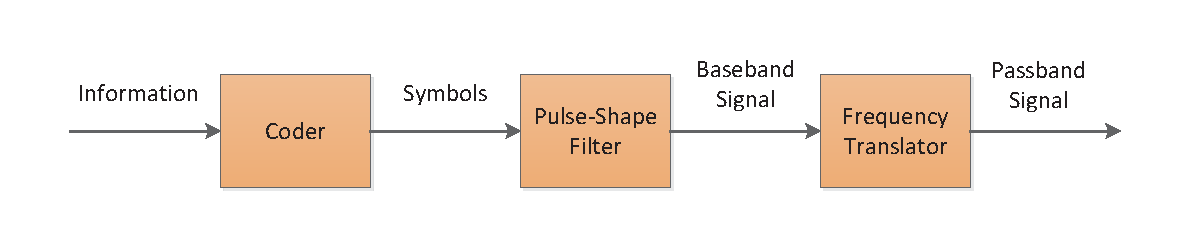
\includegraphics[scale=0.8]{Transmitter.eps}
\caption{Basic transmitter outline, converting information or data to a easily recoverable signal by the receiver.}
\end{figure}

The transmitter's sole purpose is the send data that is convenient for the receiver to understand, and allow others to use the transmission medium as well.  The coding phase of the transmitter can have many features and purposes, but simply it will encode data into a symbol with a form of redundancy or scheme that will help the receiver reconstructed the information more easily.  Next the pulse-shape filter is used to help separate data and help maximize the SNR at the receiver.  This filtering can be done with an assortment of filter shapes, but the most popular is the raised square-root cosine filter.  After pulse-shaping, the signal is translated into frequency information and unconverted to a high RF with a carrier signal.  The translation is done with a modulation scheme such a binary phase-shift keying (BPSK) or pulse amplitude modulation (PAM).  The is up-converted by mixing the signal with a sinusoid, seen by Equation \eqref{mixing}.

\begin{equation}[!ht]\label{mixing}
cos(x)cos(y)=\frac{(cos(x+y)+cos(x-y))}{2}
\end{equation}

This done because low-frequency signals such as speech, music, or digital data can be much more efficiently transmitted at higher frequencies \cite{9}.\\

Now let us discuss the receiver.  At the system level, a modern digital receiver can be broken down into a small set of distinct categories or operations: carrier synchronization, timing synchronization, equalization, and frame synchronization, as outlined in Figure \ref{Receiver_Blocks}.  These sections work together in series to provide smooth transmission of data, and many techniques exist within theses categories to accomplish its goal.  In most communication systems, after the radio frequency (RF) front-end, the first operation done on the received signal is frequency compensation and down conversion.  This compensation needs to accomplished because non-idealities and differences exist between the transmitter's and receiver's oscillator.  Therefore this is continually compensated for and corrected.  Carrier recovery can be accomplished using several methods that include but are not limited to: squared difference loops, phase-locked loops, costas loops, and decision-directed phase tracking \cite{9}.\\

\begin{figure}[!ht]\label{Receiver_Blocks}
\centering
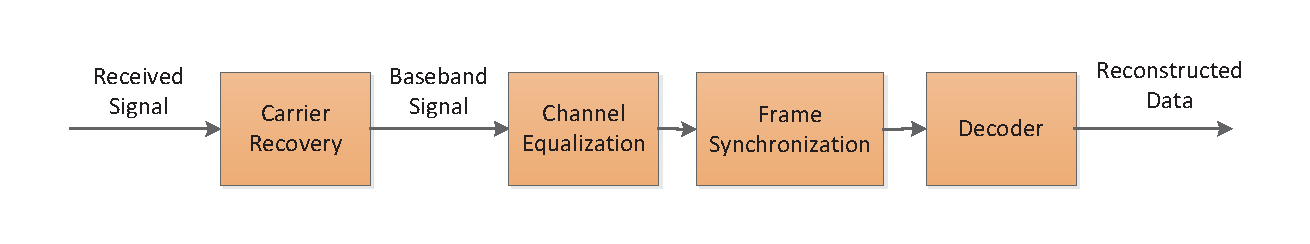
\includegraphics[scale=0.7]{Receiver.eps}
\caption{Basic wireless receiver outline, with four primary blocks.  All designed to remove corruption caused by the wireless environment and translate transmitted signals back to desired data.}
\end{figure}

After carrier recovery, the signal is pulse-shaped with the same filter shape used at the transmitter.  This technique will help to maximize the SNR of the signal.  Then the signal must be corrected again for timing.  The purpose of timing recovery is to choose the instants at which to sample the incoming signal.  This is generally done through a interpolation mechanism of the transmitted signal.  Since at the transmitter the signal is upsampled to symbols, a single data point or bit is represented by several received data points.  Therefore these points can be interpolated together for a more accurate estimate of the original data.  Timing recovery also can be done with one of several methods including: output power maximization, Mueller-Muller method, or decision-directed.  Generally, they utilize their own interpolation algorithm, such as sinc-interpolation \cite{9}.\\

After this point the receiver designs can vary greatly, as the design in this thesis will present, because this is where most of the digital signal processing (DSP) will take place.  This section, call Equalization, is responsible to correcting any effect the channel has on the signal. This includes multi-path, noise, 	and other distortions that cause inter-symbol interference (ISI).  Equalizer implementations are designed to compensate for types of disturbances that occur using certain systems.  The equalizer stage is most often coupled with the frame synchronization stage such that the equalizer itself can adapt to changing conditions.  This is known as soft decision making.  Equalizer techniques include but are not limited to: LMS , decision-directed, dispersion-minimizing \cite{9}, Viterbi \cite{viterbi}, blind, and turbo equalizers \cite{turbo}.\\  

\subsection{Equalization}

Equalizers can be considered the most complicated design of an entire communication system since they combat a series of distortions.  The primary result of these distortions is called inter-symbol interference (ISI).  ISI simply means that symbols interact with one another in the channel space and cannot be considered independent from one another.  Since this interference is generally considered a frequency selective disruption or dispersion a filter needs to be employed to reverse such effects.  This filter must be adaptable because the channel distortion cannot be know prior to transmission.\\  

As listed in the previous section, many equalizers exists and operate under specific conditions.  Here several linear equalizers will be discussed in detail including maximum-likelihood sequence detection, adaptively trained equalizer, and decision-directed linear equalization.  The goal of all of these equalizers is to find a finite impulse response (FIR) filter that when convolved with the received signal produces the original transmitted data \( \boldsymbol{\hat{X}}=\bf{Y} * \bf{G} \).  Figure \ref{FIR_filter} outlines a typical FIR structure for which the equalizer will create the appropriate coefficients \(b_{0},b_{1},..., b_{n} \).  These equalizers also examine the condition of an additive white Gaussian noise (AWGN) channel, and uncorrelated or independent interferers.\\

\begin{figure}[!ht]\label{FIR_filter}
\centering
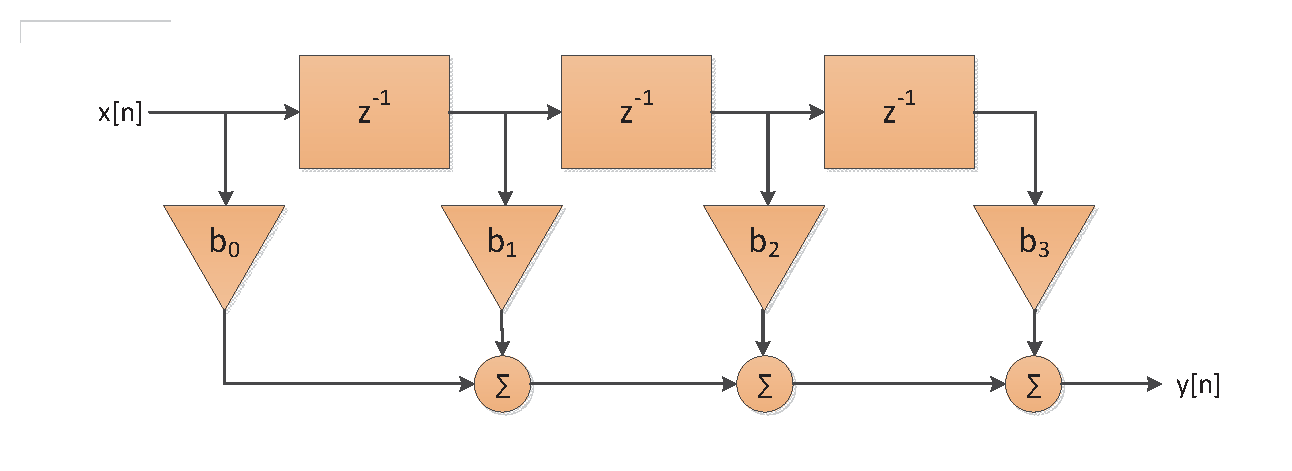
\includegraphics[scale=0.7]{FIR_filter.eps}
\caption{FIR Filter Structure}
\end{figure}

The Zero Forcing Equalizer (ZFE) uses peak distortion criteria to determine equalizer coefficients.  The ZFE produces zero ISI at its output.  If \(H_{c}(f)\) is assumed to be the effects of the channel, the ideal equalizer would be \( H_{eq}(f)=\frac{1}{H_{c}(f)}\).  This can also be consider the inverse of the channel.  The filter coefficients are modeled as weighted pulses convolved with the channel, which can be expressed as Equation \eqref{weighted}.  Here \(b\) represents the weighted filter taps, \(p_{r}\) represents the input signal and \(p_{eq}\) represents the output of the filter.

\begin{equation}\label{weighted}
p_{eq}(t) = \displaystyle\sum_{k=-M}^{M} b_{k}p_{r}(t-kT)
\end{equation}

Unfortunately, the ZFE has a large disadvantage; it cannot compensate for small amounts of noise.  Technically, the ZFE will amplify all noise of the received signal, and if any elements of the channel matrix are considerably small, then the equalizer becomes unstable. Therefore this is generally considered a more theoretical or elementary equalizer formulation.  To overcome this problem the zero ISI condition must be relaxed allowing for noise which if small can easily be overcome by such operations as quantization or decision making.  The Linear Minimum Mean Squared Error Filter (LMMSE) takes this relaxation into account \cite{spinger}.\\ 

The LMMSE assumes that the symbols are uncorrelated with one another and uncorrelated from the noise in the channel.  This approach tries to minimize the mean square error, a common measure of estimator performance.  The estimator is defined as \(\hat{x}_{MMSE}(y)=E{x|y}\), where we are given the received signal \(y\) and must guess or estimate \(x\), which was transmitted originally.  If \(x\) and \(y\) are jointly Gaussian, then the LMMSE will be linear.  This function or equalizer design minimizes the mean square error.  To simplify further an extension to random vectors can be examined.  An estimate can be made for the original vector \(x\) represented by \(\hat{x}\), resulting in the linear equation \(\hat{x}=ay+b\).  \(a\) and \(b\) represent the coefficients to be selected for the estimator.  The LMMSE will minimize the mean square error shown in Equation \ref{mse}:

\begin{equation}\label{mse}
 MSE = \|x-\hat{x}\|^{2}
\end{equation}

Besides these linear equalizers outlined, an adaptive approach can also be considered.  The Least Mean Squares (LMS) or Gradient Descent algorithm utilizes a traditional technique for minimizing the error in a signal.  This method is historically known as the "Method of Steepest Decent" or a very closely related algorithm called "Newton's Method". By calculating the error of each received symbol, this can be fed back into the system for future symbols.  This error will shape the equalizer's filter coefficents to match the inverse of the channel.  The equations \ref{lms_eq}, \ref{lms_eq2}, and \ref{lms_eq3} outline the LMS algorithm.

\begin{equation}\label{lms_eq}
y[n]=w[n]^{H}u[n]\\
\end{equation}

\begin{equation}\label{lms_eq2}
e[n]=d_{n}-y[n]\\
\end{equation}

\begin{equation}\label{lms_eq3}
w[n+1]=w[n]+\mu u[n]e^{*}[n]\\ 
\end{equation}

In these equations: \(w\) represents the adaptive filter coefficients, \(u\) the input signal, and \(d\) the known signal.  \(\mu\) acts as the algorithm's step-size determining how quickly it will converge.  It must also be considered that the larger the step-size the higher the probability it may become unstable.  As long as the channel's effects are slow changing, this equalizer can easily maintain up to date estimates while corrupting as little of the data as possible.\\  

All of the methods proposed so far require \textit{known} data (\(d_{n}\) in Equation (\ref{lms_eq2}) to correct against.  This data is called training data and generally comes in the form of a preamble in a frame.  The preamble is added to the beginning of each frame so the equalizer can learn from the effects on that specific data.  The preamble is the same for all frames and is always used so the equalizer will always be learning.  However, what happens when data is unknown in the frame, such as the payload portion of the frame.  This is where blind equalization is employed.\\

Several blind equalizers exist but an extension of the LMS equalizer for blind situations will be examined here called the decision-directed equalizers \cite{9}.  For a blind equalizer to operate an error generation mechanism must be evaluated, but since the data symbols are unknown, a decision device must be used in place.  This decision device is a quantization method and the error is generated from this quantization.  This error generation is extrapolated from expression: 
\(e = \frac{1}{2}(sgn(y[k]-y[k])^{2}\)
Where the \(sgn\) function returns 1 for positive numbers and -1 for negative numbers.  This expression is quite similar to the original LMS implementation except instead of a known symbol the data is quantized using the sign function.  This type of quantization using the sign function is only applicable with binary modulation schemes such as BPSK.  This equalizer method is usually combined with a training equalizer method in practice, since if a nearly closed eye is observed, when using an eye diagram, this equalizer cannot open it by itself.  An example of such an eye diagram is shown in Figure \ref{eye_closed}, and clean/open eye diagram can be seen in Figure \ref{eye_clean}.\\

\begin{figure}\label{eye_clean}
\centering
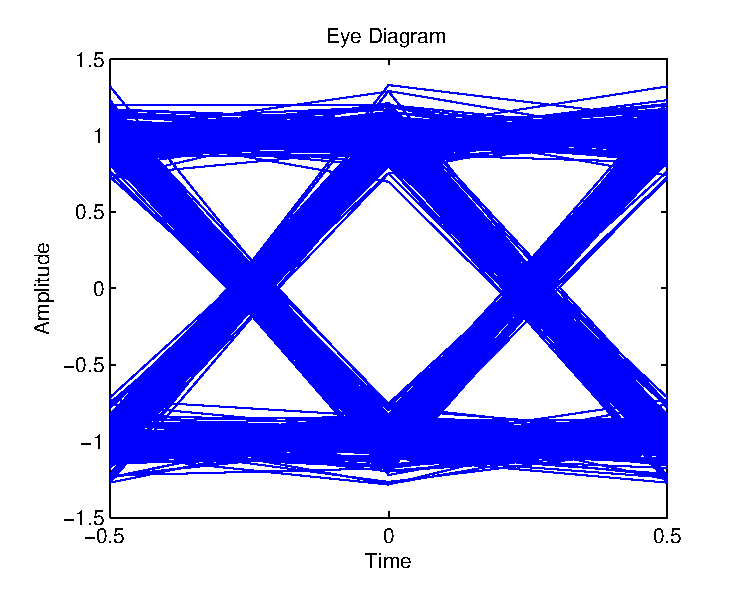
\includegraphics[scale=0.8]{eye_clean.eps}
\caption{Adequate timing recovery produces open eye, which clearly defines the received symbols in time.}
\end{figure}

\begin{figure}\label{eye_closed}
\centering
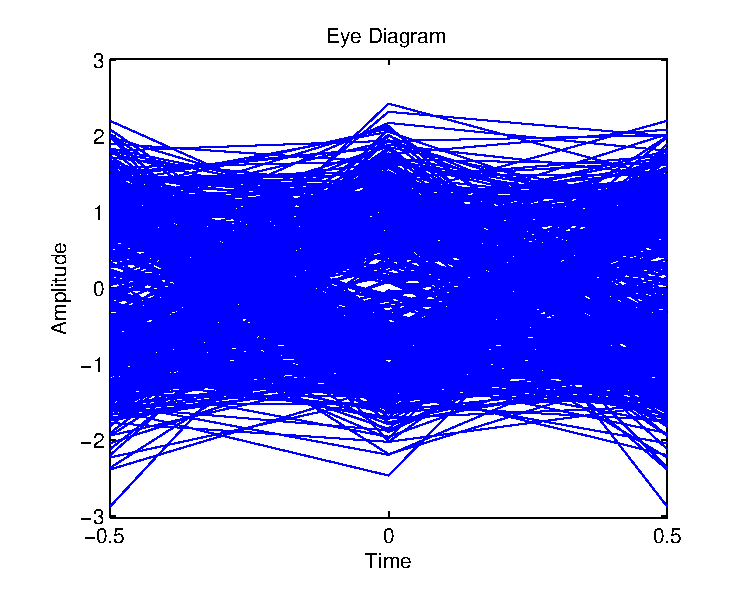
\includegraphics[scale=0.8]{eye_closed.eps}
\caption{Poor timing recovery produces a closed eye, identifying that the signal cannot be recovered unless corrective measures applied.}
\end{figure}

In this section, we have examined several equalizer techniques while outlining their advantages and disadvantages.  Most techniques require some training mechanisms to operate under heavy channel distortion, and blind techniques such as decision-directed equalization will fail under these conditions.  Unfortunately, such training data can take considerable resources, and lower overall data throughput.  In practice as much as 20\% of frame information is training.  Therefore other techniques must be considered to help overcome this obstacle.\\


\subsection{Superimposed Training Equalization}

As mentioned in the previous section, many implementations exist for equalizer designs, but this thesis will examine the effectiveness of superimposed training symbols in frequency selective channels.  In traditional equalizers, channel estimation is achieved through the use of training data or pilot symbols.  These symbols are both known to the transmitter and receiver, providing the basis for an estimate.  In these equalizers all training symbols are placed at the start of a frame, with \cite{16} showing that under high SNR training-based schemes are capable of capturing most of the channel capacity, while under low SNR they are highly suboptimal.  Superimposed equalizers try to overcome this problem along with others to provide more optimal estimates.  Superimposed equalizers physically add training symbols to the data stream instead of concatenating symbols, saving valuable bandwidth \cite{16}.  To accommodate such pilots, energy must be shared among the data and hidden pilots \cite{Ghogho}.  Reference \cite{19} shows that for a transmitter of fixed power, with an additive pilot sequence, the decrease in data signal power is equal to: \[ K_{loss}=\frac{E[\|s(k)\|^{2}}{E[\|s(k)\|^{2}]+E[\|u(k)\|^{2}]}\] equivalent to \(10logK_{loss}dB\) in signal to noise ratio (SNR).  With \(s(k)\) representing the source signal, and \(u(k)\) representing the received signal.  Other disadvantages include an increased signal envelope fluctuation that can be undesirable in nonlinear transmit power amplifiers \cite{17}.\\  

At the receiver, channel estimation can be done using several techniques in both the frequency and time domain.  Reference \cite{17} examines a time domain approach for synchronized averaging of the received signal.  It is important to note that this synchronization is not related to transmitter and receiver synchronization.  References \cite{17} and \cite{18} both assume that the signal \( \bf{x}(n)\) and noise \( \bf{v}(n) \) have zero mean and \(E[m_{x}(n)] = \bf{d}(n) = \bf{p}(n) \ast \bf{h}(n)\).  Therefore, since \(\bf{p}(n) \) is the known superimposed periodic pilot sequence, \(\bf{h}(n)\) can be determined.  Note that \(\bf{h}(n)\) is generally considered frequency selective, and such channels can be quite difficult to deal with especially with multi-path.  Multi-path interference is a distortion caused when copies of the original signal arrive at the receiver delayed on top of the originally received non-delayed signal.  This delayed signals essentially take other paths to the receiver, and this interference's manifestation is commonly called \textit{ghosting} in such applications as television broadcasts \cite{ghost}.\\

Superimposed equalizers are able to better compensate for large multi-path channels because they can spread their training symbols throughout the signal itself.  This spreading not only provides a spreading in time but also in other dimensions such a frequency.  Therefore, if the training symbols are chosen correctly and placed correctly, they can then be spread across the frequency spectrum efficiently and capture its selectivity.  Before the pilots can be examined, the channel must be defined.  The channel is of block length \(N\), and the channel is also time invariant across single blocks, but variable across blocks.  The memory of this channel is of maximum length \(L-1\), and the impulse response of the channel is defined as \(\textbf{h}=[h_{0},...,h_{L-1}]^{T}\).  Since there are \(N\) blocks in the channel, the channel matrix \(H\) is modeled as an \(N x N\) circulant matrix, with the received signal as expressed as:

\begin{equation}
\textbf{x}=\textbf{H}\textbf{s}+\textbf{v}
\end{equation}

Here, \(\textbf{v}\) is assumed to be zero mean white noise.  The vector \(\textbf{s}\) is a combination of known training symbols and unknown data.  The optimal placement for such training is where the channel undergoes non-ergodic fading considered here \cite{20}.  Reference \cite{16} continues on to say that optimally, assuming symbols are placed in clusters of length \(\alpha \ge 2L+1\), this scheme is quasi-periodic.  The variable \(\alpha\) represents the cluster size in this scenario.  It is also important to note that this placement makes sure that the training is always orthogonal.\\

Another effect that must be considered is how these training symbols interfere with the data itself, and is the training symbols dependent on the data or even the modulation scheme.  Reference \cite{Ghogho} examines this aspect and proposes solutions that provides a data independence condition.  As explained previously, since the training data is periodic it can be placed in equispaced frequency bins, while data is spread across all frequency bins.   Therefore, the pilot must be designed to distort the data vector of the discrete Fourier transform to zero.  In the superimposed training data case, this is done by using the cyclic mean of the data.  Therefore, all that needs to be done is the removal of the cyclic mean \(\textbf{e}=\textbf{Jw}\).  Note that \(\textbf{J}\) is the Kronecker product of an identity matrix and the fractionally spaced locations of the pilot tones.  Therefore, at the pilot frequency only the training symbols are visible for the channel estimation.  Formally here is the transmitted, or precoded, result including pilots and data: \( \textbf{s}= (I-\textbf{J})\textbf{w}+\textbf{c}  \).\\


In summary, research on superimposed training focuses primarily on the training symbol generation for a certain type of communication systems design from single transmission to multiple-input multiple-output (MIMO).  Unfortunately, little to no physical implementations exists for such systems.  This is true because of the synchronization issue that exists when using superimposed training symbols.  Since they are directly placed with transmission data it can be difficult to determine their locations in a sequence blindly, which is done in real world systems.  This problem must be considered when physical implementations are proposed.\\

\section{Spectral Subtraction}

Now that methods of reconstructing information distorted by the channel itself has been discussed, we can now focus on spectral removal of known signals without demodulation.  Such a technique is needed to improve the effectiveness of equalization operations done downstream, while limiting corruption to the desired signals themselves.  In this thesis a new application for a relatively standard technique was examined, called Spectral Subtraction (SS).  The SS technique was first published in 1979 by Steven Boll \cite{boll}. SS is formally used to reduce ambient noise in audible sources, improving the overall quality and intelligibility of digitized speech.  It is a dominant speech processing algorithm and many extensions including \cite{SSEXAMPLE}, \cite{SSEXAMPLE2}, and \cite{SSEXAMPLE3}.  Due to the large amount of literature and investigation into the SS process it was assumed to be a solid option for removing unwanted signals in the spectrum.\\

SS primarily was designed for audio signal processing, small bandwidth signals roughly from 20Hz to 20,000Hz.  Many forms of SS exist, but the approach examined here is Magnitude Spectral Subtraction (MSS).  It works by first generating an estimate of the noise in the signal itself, which is usually attained at the first first few seconds of the signal itself.  This noise is then subtracted, as the name suggests, from the rest of the signal.  Mathematically, let us explain this further.  The received signal is assumed to be a combination of two signals, the transmitted and the noise itself \(y(t) = x(t) + n(t)\).  Next the power spectral densities (PSD) are calculated for these components:

\[ E\{|Y(e^{jw}|^{2}\}= E\{|X(e^{jw}|^{2}\} + E\{|N(e^{jw}|^{2}\} + 2E\{|X(e^{jw}|^{2}\}\{|N(e^{jw}|^{2}\}\]
\[ E\{|Y(e^{jw}|^{2}\}= E\{|X(e^{jw}|\} + E\{|N(e^{jw}|\}  \]

Here \(Y(e^{jw})\), \(X(e^{jw})\), and \(N(e^{jw})\) represent the frequency domain transform of the given signal, also \(x\) and \(n\) are uncorrelated.  Since at points when the desired signal is not present in the spectrum, a silent period, the measurement for \(N\) is taken and then subtracted from the entire received signal \(E\{|X(e^{jw}|\}= E\{|Y(e^{jw}|\} - E\{|N(e^{jw}|\}\).  The is noise is assumed to be quite stationary during the signal period.  Therefore, the original estimate \(\hat{N}\) can be quite accurate.\\

\subsection{Residual Noise}

As a result of the changes over time in the noise spectrum (whether power or magnitude) around its expected value, there is always some difference between the actual noise and its mean value. Hence, some of the noise remains in the spectrum in the case that the value of noise is greater than its mean and some of the speech spectrum also is removed in the case that the estimate of noise to be greater than the actual value of noise. The latter produces negative values in the spectrum. These negative values are prevented or set to a floor (sometimes zero) using different techniques. The overall effect puts noise in the output signal known as residual. The narrow band relatively long-lived portion of residual noise is sometimes referred to as musical noise \cite{mnoise}.

A close examination of musical noise, shows that peaks and valleys exist in the short term power spectrum of white noise.  These frequency locations for one frame are random and they vary randomly in frequency and amplitude from frame to frame. When a smoothed estimate of the noise spectrum is subtracted from the actual noise spectrum, all spectral peaks are shifted down while the valleys are set to zero. Therefore, after this subtraction sharp peaks remain in the noise spectrum and pre-existing ones can be sharpened. The wide peaks are generally estimated as time varying broadband noise. The narrower peaks, which are relatively large spectral distances because of the deep valleys that define them, are perceived as time varying tones which are generally referred to as musical noise \cite{berouti}.

Therefore, \cite{boll} continues by introducing a ``smoothing'' technique before the signal is convert back into the frequency domain.  Two additional parameters are introduced: The parameter \( \alpha \) the over-subtraction coefficient, and \(\beta\) the noise floor lower bound.  \(\alpha\) is used to provide a more aggressive subtraction to the signal, attacking high peaks which are generally a result of high noise and an inaccurate initial estimate.  The second parameter \(\beta\) is used to fill in the valleys of the signal.  Since if an over-subtraction takes too much signal it can cause valleys in the spectrum below or above the zero threshold.  This value is used to simply quantize values within its +/- limits.  As a result these operations together produce a smoother signal removing much of the residual noise from just a plain subtraction.  Reference \cite{boll} provides several results examining the benefits of such a technique.\\  


\section{Software Defined Radio}

Now that the signal processing techniques have been discussed, a platform for implementation is needed.  The alley chosen for this thesis is to utilize a new hardware frontier called Software-Defined Radio, which will be discussed in this section.\\

For the past two decades there has been a paradigm shift is the definition of a radio device.  The conversation has to do with the question of where hardware ends and where software begins.  The term Software Defined Radio, coined by Dr. J. Mitola III,  defined as a set of digital signal processing (DSP) primitives, a meta-level system for combining the primitives into communication system functions (transmitter, channel model, receiver, etc.), and a set of target processors on which the software radio is hosted for real-time communications \cite{21}.  Dr. Mitola understood how software provided the flexibility that hardware never could, and as time made it more mailable SDR would become dominant.\\

SDRs can be flexible enough to avoid the ``limited spectrum'' assumptions of designers of previous kinds of radios, in one or more ways including: Ultrawideband transceivers, cognitive radio, dynamic mesh networks, software-defined antenna arrays among others \cite{22}.  One of the first SDR implementations was a project called ``SpeakEasy''.  The original purpose of SpeakEasy was to use programmable processing to emulate more than ten existing military radios, operating in frequency bands between 2 MHz and 2 GHz \cite{23}.  Therefore with this single radio, the operator could talk to ten radios operating under ten different standards.  As simple enough idea, but unfortunately the implementation left much to be desired.  For example, physically the device encapsulated the entire back of a common pickup truck \cite{23}.  This might be great for a ground station that does not move, but for a mobile unit this was highly impractical.  Secondly, in 1992 field programmable gate arrays (FPGA) required significant time, comparatively to re-flash or change their operational parameters.  Again, this also limited SpeakEasy's flexibility.\\

\begin{figure}\label{sdr_overview}
\centering
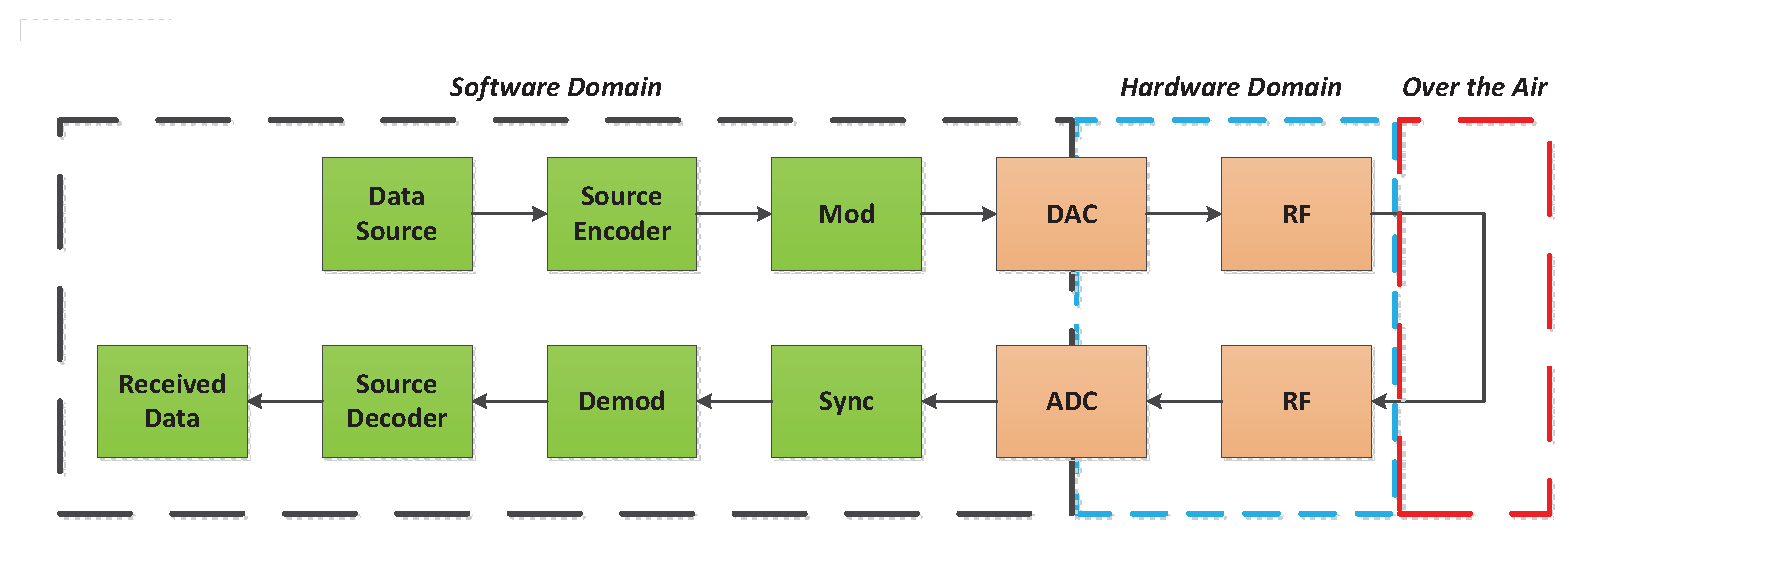
\includegraphics[scale=0.8]{sdr_overview.eps}
\caption{Software Defined Radio push all the adaptive elements and data manipulation operation into software.  The goal of SDR is to provide or define all of the radio operation in software.}
\end{figure}

Today, the main target implementations are within cellular base stations and military applications such as the JTRS project.  The JTRS or Joint Tactical Radio System, was a program of the US military to produce radios that provide flexible and inter-operable communications \cite{JTRS}. Examples of radio terminals that require support include hand-held, vehicular, airborne and dismounted radios, as well as base-stations\cite{24}.  Again, this project still has limited results and many setbacks have occurred.  Commercially, from a wide spread penetration standpoint, SDR is still many years away due to the size and cost of current devices.  The two barriers to this are speed and size.  To provide enough data throughput, modern SDRs need to quite large physically, which is a serious drawback in many applications.   Aside from these limitations, SDRs provide excellent flexibility especially in a laboratory and proof of concept environment.  Rapid prototyping is an obvious place where such radios shine, allowing massive changes without hardware modification.  To support this flexibility several software packages have been constructed around the SDR concept, allowing for aggressive prototyping.  The two examples discussed here were selected because of operability with the selected hardware, which will be discussed future in chapter 3.\\

\subsection{GNU Radio}

The first software package to be discussed by this thesis is GNU Radio.  GNU Radio provides the reconfigurable signal processing blocks that are necessary for software defined radios. GNU Radio is an open source project allowing for SDR developers to develop unique signal processing blocks and SDR systems.  GNU Radio was started in 2001, originally forked from the SpectrumWare project developed at the Massachusetts Institute of Technology \cite{spectrumware}.  Since 2001, the code base has undergone massive changes, containing almost no code from the original SpectrumWare project.  Physically the code consist of three languages Python, C++, and SWIG.  Python provides the overarching control of the system or program, while C++ provides the actual signal processing blocks and mathematics.  SWIG is a wrapper for C++ which allows Python to dynamically wrap around C++ and control or compile with it.  A diagram below better illustrates this architecture.  It is also important to mention that there as significant paradigm shifts in the community, pushing more and more code to Python rather than C++, due to its easier programming syntax and structure.\\

\begin{figure}\label{gnr_struct}
\centering
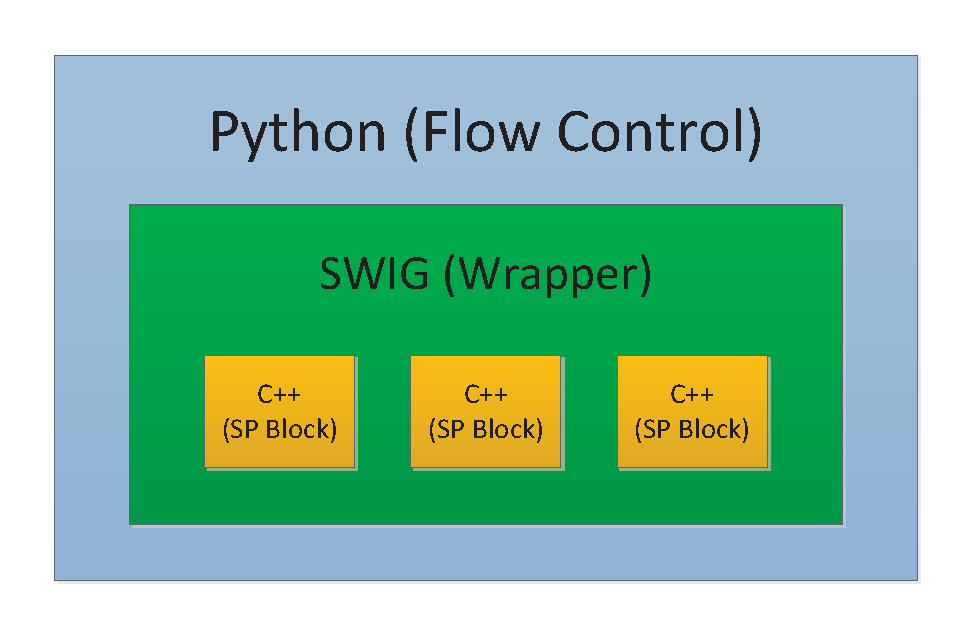
\includegraphics[scale=0.8]{gnr_outline.eps}
\caption{GNU Radio code structure based on signal processing C++ blocks and controlling, through SWIG, Python layers.}
\end{figure}

GNU Radio provides a very structured framework of flow design.  Data processing segments are extremely self contained to minimize error propagation during system debugging.  Since the software is open-source full access to all code is provide, giving low-level access to all operation within GNU Radio.  Much of the actions have been abstracted to limited the knowledge of the lower layers, but if specific actions are required for an application.  Then serious depth or knowledge is needed about the overall project's structure, which is quite overloading.\\

\subsection{MATLAB}

MATLAB is an extremely well known engineering, mathematical, biological, and financial software suite.  MATLAB provide massive data leverage and advanced communication system models and algorithm for significant data processing.  Since 2007, they have also provided hardware compliance with specific SDR platforms through their Simulink platform, and more recently within MATLAB itself \cite{matlabsdru}.  This thesis primarily utilizes the signal processing and communication system aspects of MATLAB, since MATLAB cannot fully utilize all aspects of the chosen hardware.  It is important to note under alternate constraints, MATLAB can provide adequate performance directly interfacing with hardware, especially when accessing its targeting features seen here \cite{matlabtargeting}.  Figure \ref{sdru_example} shows an example of a common MATLAB SDR model through Simulink.\\

\begin{figure}[!ht]\label{sdru_example}
\centering
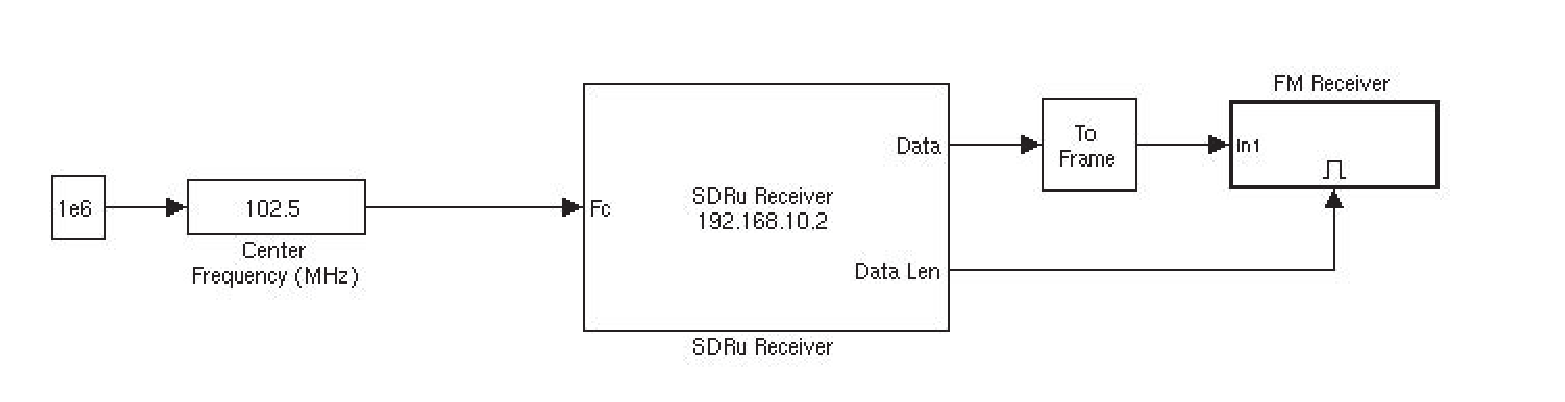
\includegraphics[scale=0.5]{sdru_example.eps}
\caption{Sample SDRU MATLAB model created in Simulink.  This model has the ability to demodulate and play FM radio stations when using a USRP device.}
\end{figure}

MATLAB provides allow connection to a USRP device through MATLAB directly of with Simulink.  The device simply acts as a real-time data source complementing their signal processing and communications toolboxes very well.  Rather than full implementations like GNUR Radio, MATLAB focuses on signal analysis rather than real-time performance.  The primary limitation is the single threaded nature of MATLAB and Simulink, which is slowly being improved upon for the SDR application.\\

\subsection{Reference Comparison}

It is important to compare GNU Radio and MATLAB, from a user's perspective they perform quite differently.  Firstly GNU Radio, is extremely fast, will the ability of sustaining the maximum throughput of the selected hardware.  GNU Radio is also multi-threaded, and while maintaining high throughput and complete background tasks on multi-core machines quite easily.  This performance has a cost, comparatively GNU Radio has an extremely learning curve and debugging can be challenging.  However if you need the performance, GNU Radio is your option, providing significantly more advanced hardware support in SDR implementations.  If data analysis is more heavily desired MATLAB is the obvious choice.  MATLAB provides easy and advanced data visualization functionality, and built in tools for analysis.  Since MATLAB does not compile itself normally, it can be much easier to debug and solve problems.  MATLAB's syntax provide similar data manipulation, especially in communication system primitives.  Therefore, it can be a rather simple choice, speed or ease of use.\\ 

\section{Summary}

This chapter outlined and examined the topics of jamming and anti-jamming techniques, and provided a foundation in communication system theory and advanced equalizer design.  Secondly it setup an understanding of Software-Defined Radio, the power of such an architecture, and examples of implementations and existing software for future designs.  Next, this thesis will consider a new anti-jamming technique and design an implementation of such a system.  After the implementation is investigated, the result of specific experiments on such an implementation will be analyzed.\\


%% Implementation Section
\chapter{Implementation}
\label{ch:implementation}

\section{Overview}

Now that a significant background has been provided, the problem this thesis combats will be futher framed and defined.  This chapter outlines the proposed implementation of a receiver design, for wideband jammer scenarios and low-mobility situations.  An adaptive signal processing software solution for mitigating the effects of both intentional and unintentional jamming (including wideband jamming) through a combination of three techniques.  These include: antenna subset selection, spectral subtraction, and blind source separation (BSS), which work in conjuction with one another to extract specific transmissions from a mixture of intercepted wireless signals. The goal of the proposed solution, called BLInd Spectrum Separation (BLISS), is to enable reliable, high throughput, and robust end-to-end wireless communications, especially high capacity multimedia (voice, data, imagery) transmissions. In particular, the focus of the proposed work is the so-called ``disadvantaged user''.  These users are generally considered limited in transmission and processing power such as small-deck combatants, submarines, unmanned air vehicles (UAVs), dispersed ground units in urban and radio frequency (RF) challenged environments.  The previous research is also discussed for each section and implementation consideration are examined from this work.\\

The BLISS solution integrates three well-known adaptive signal processing algorithms found in the open literature: antenna subset selection, spectral subtraction, and blind source separation. Each of these algorithms is employed within the BLISS framework in order to enable the process of extracting individual transmissions intercepted from several mixtures of wireless signals. Although blind source separation can readily extract transmissions under ideal conditions, the BLISS system is aimed at harsh spectral envirnorments consisting of many users and in some cases jamming devices. Therefore BSS will not provide adiquate signal separation for robust throughput.  Hence, the other two algorithms, spectral subtractions and antenna subset selection will aid in this effort.\\

In previous sections it has been understood that current anti-jamming techniques cannot compensate in deterministic wideband jamming scenarios.  These scenarios must be throughly understood before a practical solution can be provided.  For this thesis, the worst case scenario will be considered for the jamming device.  For simplification a narrowband jammer will be considered as an adversary, and the transceiving devices cannot frequency hop thus remaining on the same frequency as the jammer.  The jammer has an identical modulation scheme as the friendly tranceivers and the constellation is in phase.  Finally the jammer is assumed at a similar distance and transmit power as the friendly tranceiving devices.  Under these conditions the jammer is completely orthogonal and historically impossible to remove.\\

This chapter is broken down into several sections which include a system level overview, the hardware and software choosen, signal removal evaluation, the superimposed equalizer design, and the antenna subset selection work.  Each of the systems that makeup BLISS have different purposes and goals allowing them to tackle different problems that occur.  It is important to note that these systems are at differing stages of development due to the limited time and initial development put into these blocks.\\ 

\section{System}

To provide a more straight forward explaination of the BLISS system it is appropriate to provided a system level overview.  The system's original purpose was to remove the effects of narrow and wideband jamming.  It accomplishes this goal through a series of processing blocks and a selection block.  These blocks include: the antenna subset selection (AntSS) block, spectral subtraction block, and finally the blind source separation block.  The figure below shows the interconnections between these blocks and certain modification were made from the original design of the system due to practical constraints.  These changes will be brought fourth as the blocks themselves are discussed in detail. Since an external research group is responsible to the AntSS block, it will not be throughly discussed by this thesis, but its fundimental purpose will be examined.\\

\begin{figure}[!ht]\label{bliss_system}
\centering
\includegraphics[scale=0.5]{bliss_system.eps}
\caption{Overview of BLISS System }
\end{figure}

The first step in the BLISS system is to pass through the AntSS block.  Physically this block is equipped with many antenna in groups of 4.  As the block title portrays a subset of these antennas will be selected and they will be passed on to the next block.  Precisely a \(2^{M}-to-2^{N}\) downselection from an array of receive antennas to a set of BLISS receiver inputs. Each individual AntSS board provides 4-to-2 antenna downselection through a set of RF switches.  The goal of AntSS is to provide spatial separation through an array of antennas maximizing the SNR of the wanted signal.  It is important to note that the antenna spacing must be adiquet to provide enough separation or independence, depending on the operating frequencies or wavelength of the signals themselves.  Once the appropriate antennas are selected two signals are to the spectral subtraction block.\\

The spectral subtraction block is next, which is used to removal known unwanted signal from the spectrum so the source separation block and work properly.  The original design of the spectral subtraction block is to use an existing audio technique of removing noise or signals in the frequency domain through a subtraction and smoothing technique.  This technique was discussed previously in the background section, therefore its historical literature will not be examined futher.  To enable removal of unwanted signals, the Spectral Subtraction block maintained a database of known power spectral densities (PSD) of common modulation schemes.  A recognition system would be implemented to automatic identification of the interfering signal and the block would simply subtract it out, through its already known estimate from its database.  Next the newly subtracted signal would be passed to the Source Separation System, where the signal would be unmixed.\\

The source separation block separates signals when only their mixtures are observed.  The operation is called blind, since the signal sources and mixing procedure are unknown to the receiver.  Under some conditions this constraint cannot be completely upheld.  This is true because the solutions needed to solve such an event become generally intractable.  An initial approach in this project was to use a technique called AMUSE (Algorithm for Multiple Unknown Signals Extraction)\cite{AMUSE}.  AMUSE works by first collecting an estimate of the covariance matrix of the received signal, computing the singular value decomposition of that covariance matrix, then performing several transforms on the received signal once the number of mixed received signals is known.  Then a covariance is calculated from these transformed received signals which are offset by some instance \(\tau\), and a eigenvalue decomposition is done upon these covariances.  From this decomposition the singular values are used with the transform matrix and the received signal to provide an estimate of the wanted source signal.\\

\begin{equation}\label{}
R_{y}=E[yy^{t}]
\end{equation}

\begin{equation}\label{}
z=Cy
\end{equation}

\begin{equation}\label{}
R_{z}=E[z(\tau)z(t-\tau)^{t}
\end{equation}

\begin{equation}\label{}
\hat{x}=Vhat{t}Cy
\end{equation}

It is important to note that for simplicity the mixing matrix for the original proposed solution involving AMUSE is generally constructed as a linear time invariant (LTI) system.  There is some activity occuring with nonlinear mixing, but that was considered outside of the scope of this problem.\\

\section{Hardware and Software Platforms}

Before any implementation was considered a platform needed to be choosen for the end result.  This selection provided the work flowpath for the implementation, eliminating many options.  As discussed in previous chapters, the end result wants to leverage the power of Software-Defined radios (SDR).  The hardware platform chosen was the USRP2 designed and built by Ettus Research\cite{USRP2Stats}.  These radios are readily available in the Wireless Innovation Laboratory and since the number of radios required for the design was still unknown, it was an obvious choice.  There are several software packages that support the USRP2 hardware and several will be examined in this chapter.\\

The USRP2 or Universal Software Radio Peripheral are intended to be a comparatively inexpensive hardware platform for software radio, and is commonly used by research labs, universities, and hobbyists\cite{wired}.  The USRP2 connects directly to a host computer through a Gigabit Ethernet link, which relays baseband sample that have been receiver or tobe translated.   The motherboard provides the following subsystems: clock generation and synchronization, FPGA, ADCs, DACs, host processor interface, and power regulation. Several of these component are seen in the image below.  These are the basic components that are required for baseband processing of signals. A modular front-end, called a daughterboard, is used for analog operations such as up and down conversion, filtering, and other signal conditioning. By replacing this RF daughtercard many different frequency ranges can be examined.\\

\begin{figure}\label{usrp2_full_hardware}
\centering
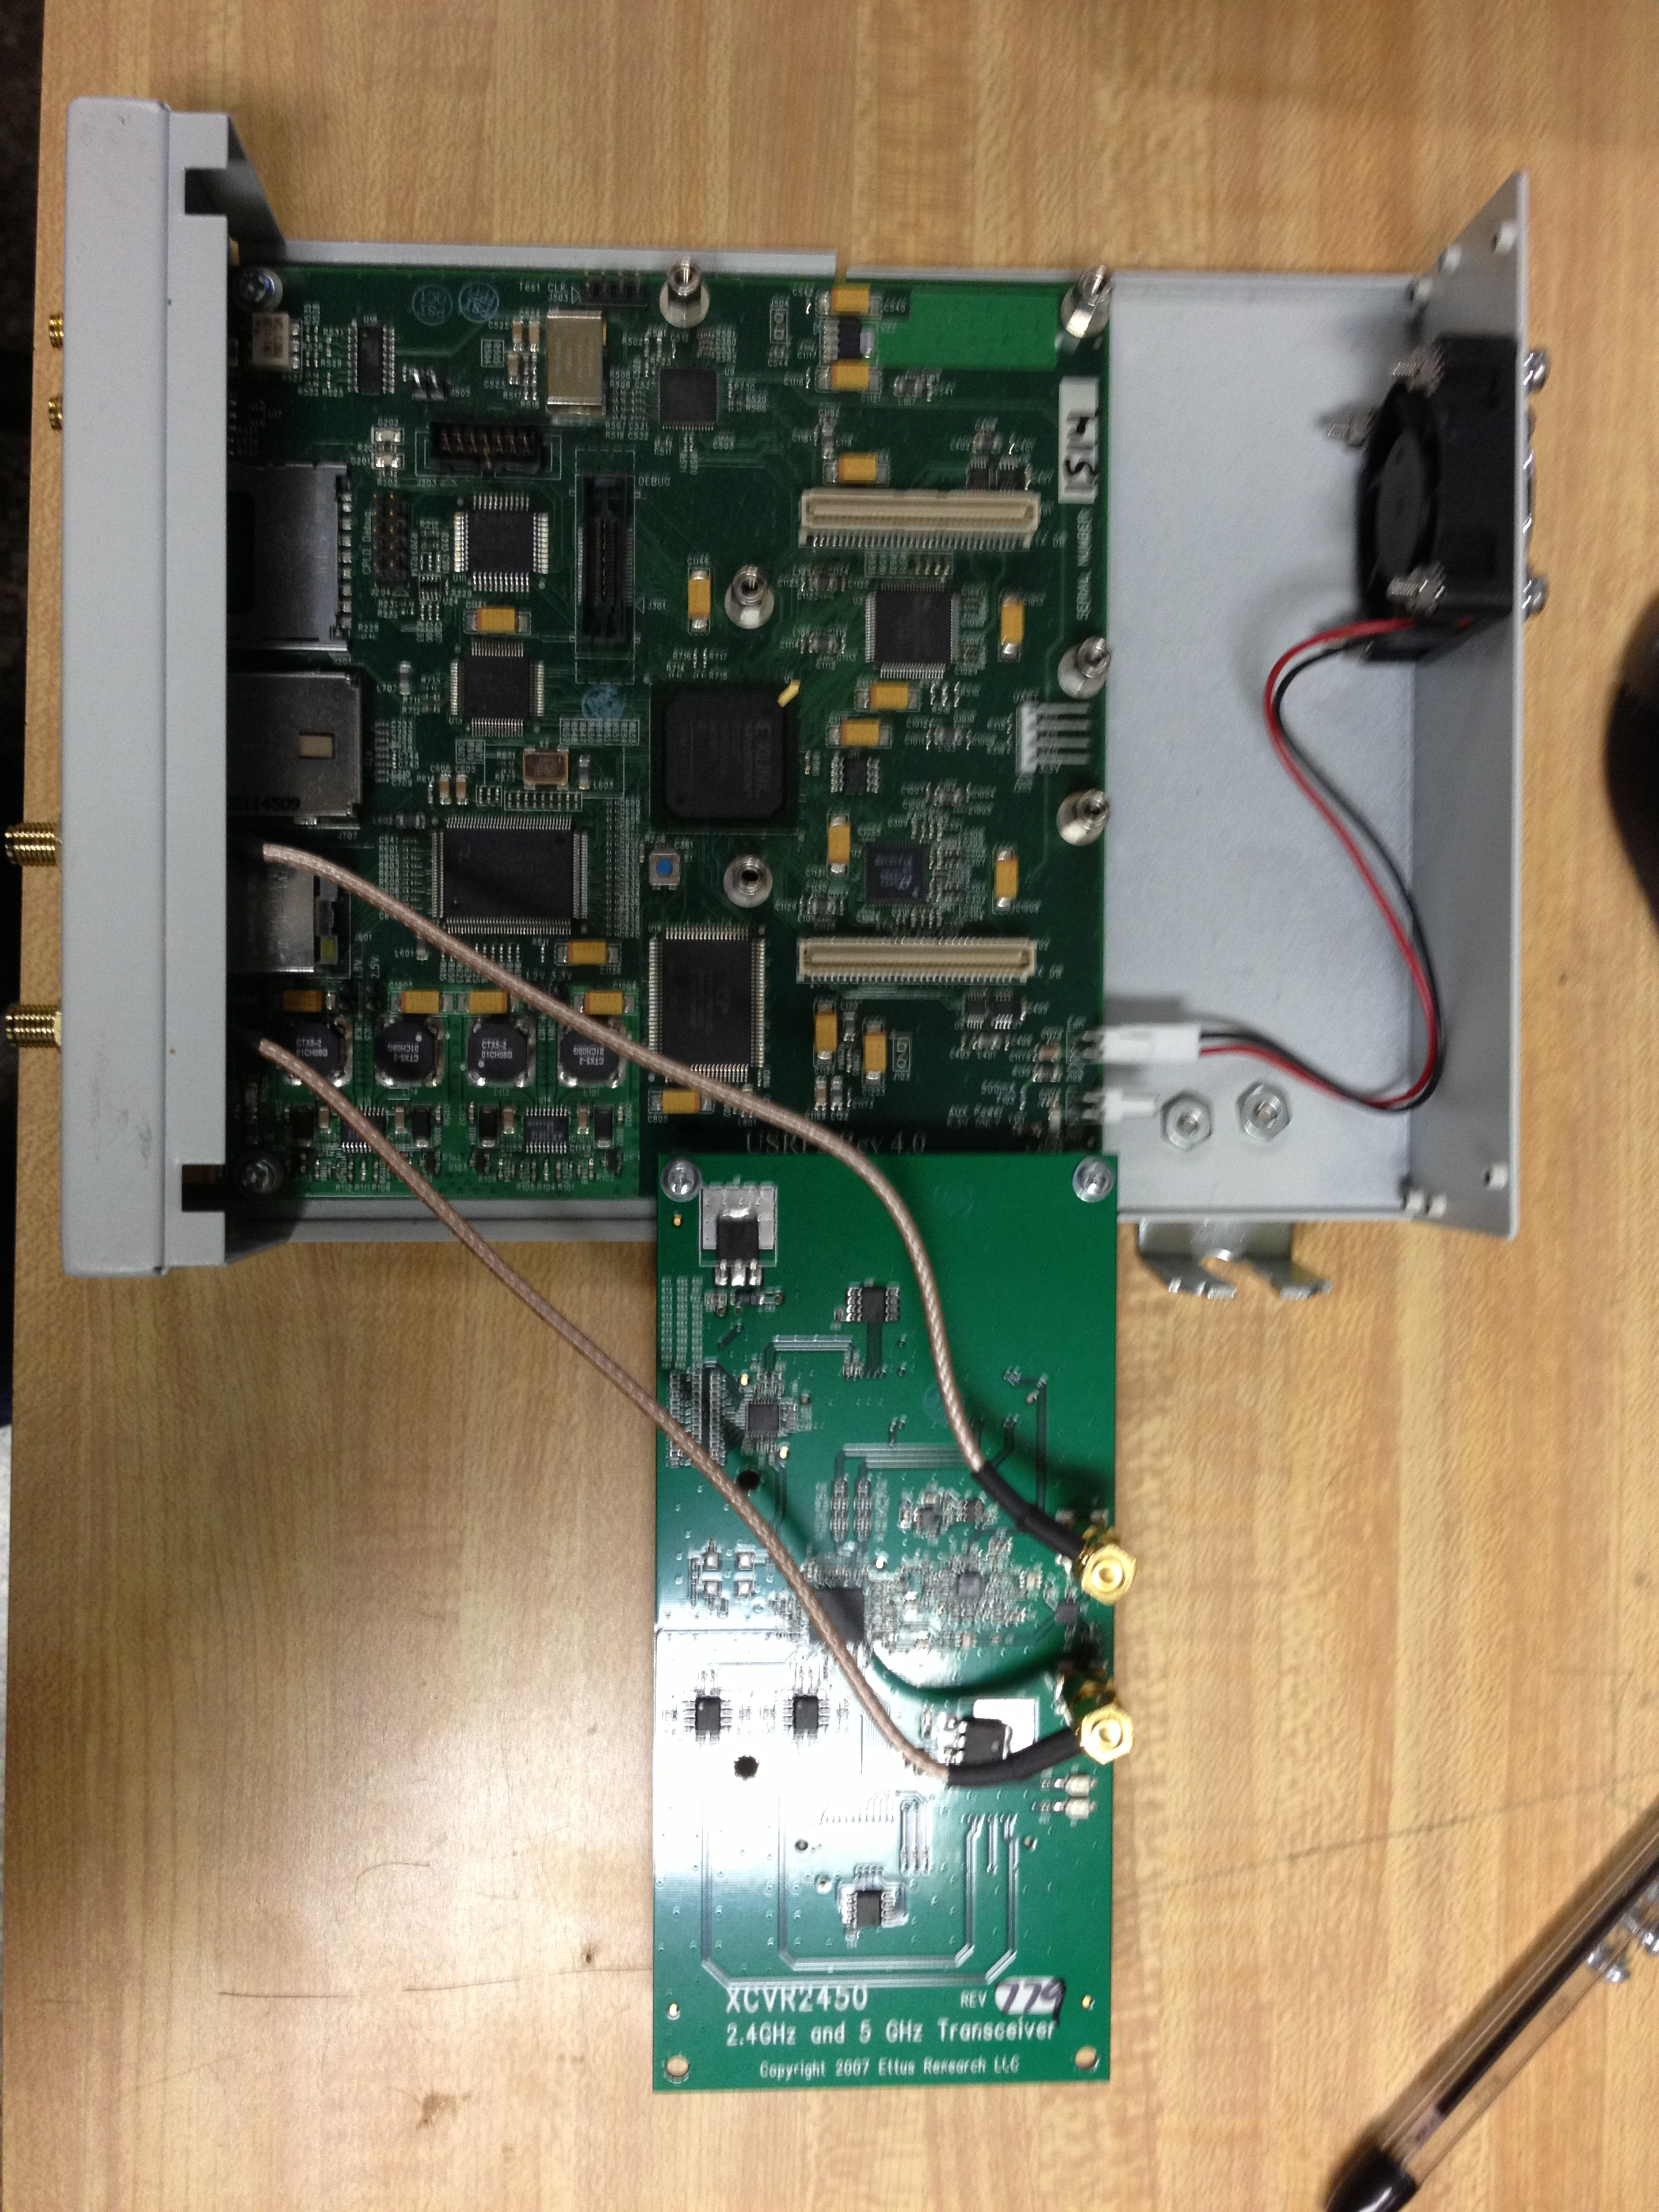
\includegraphics[scale=0.1]{usrp2_overview.eps}
\caption{Full USRP2 Hardware with Daughtercard}
\end{figure}

\begin{figure}\label{usrp2_mainboard}
\centering
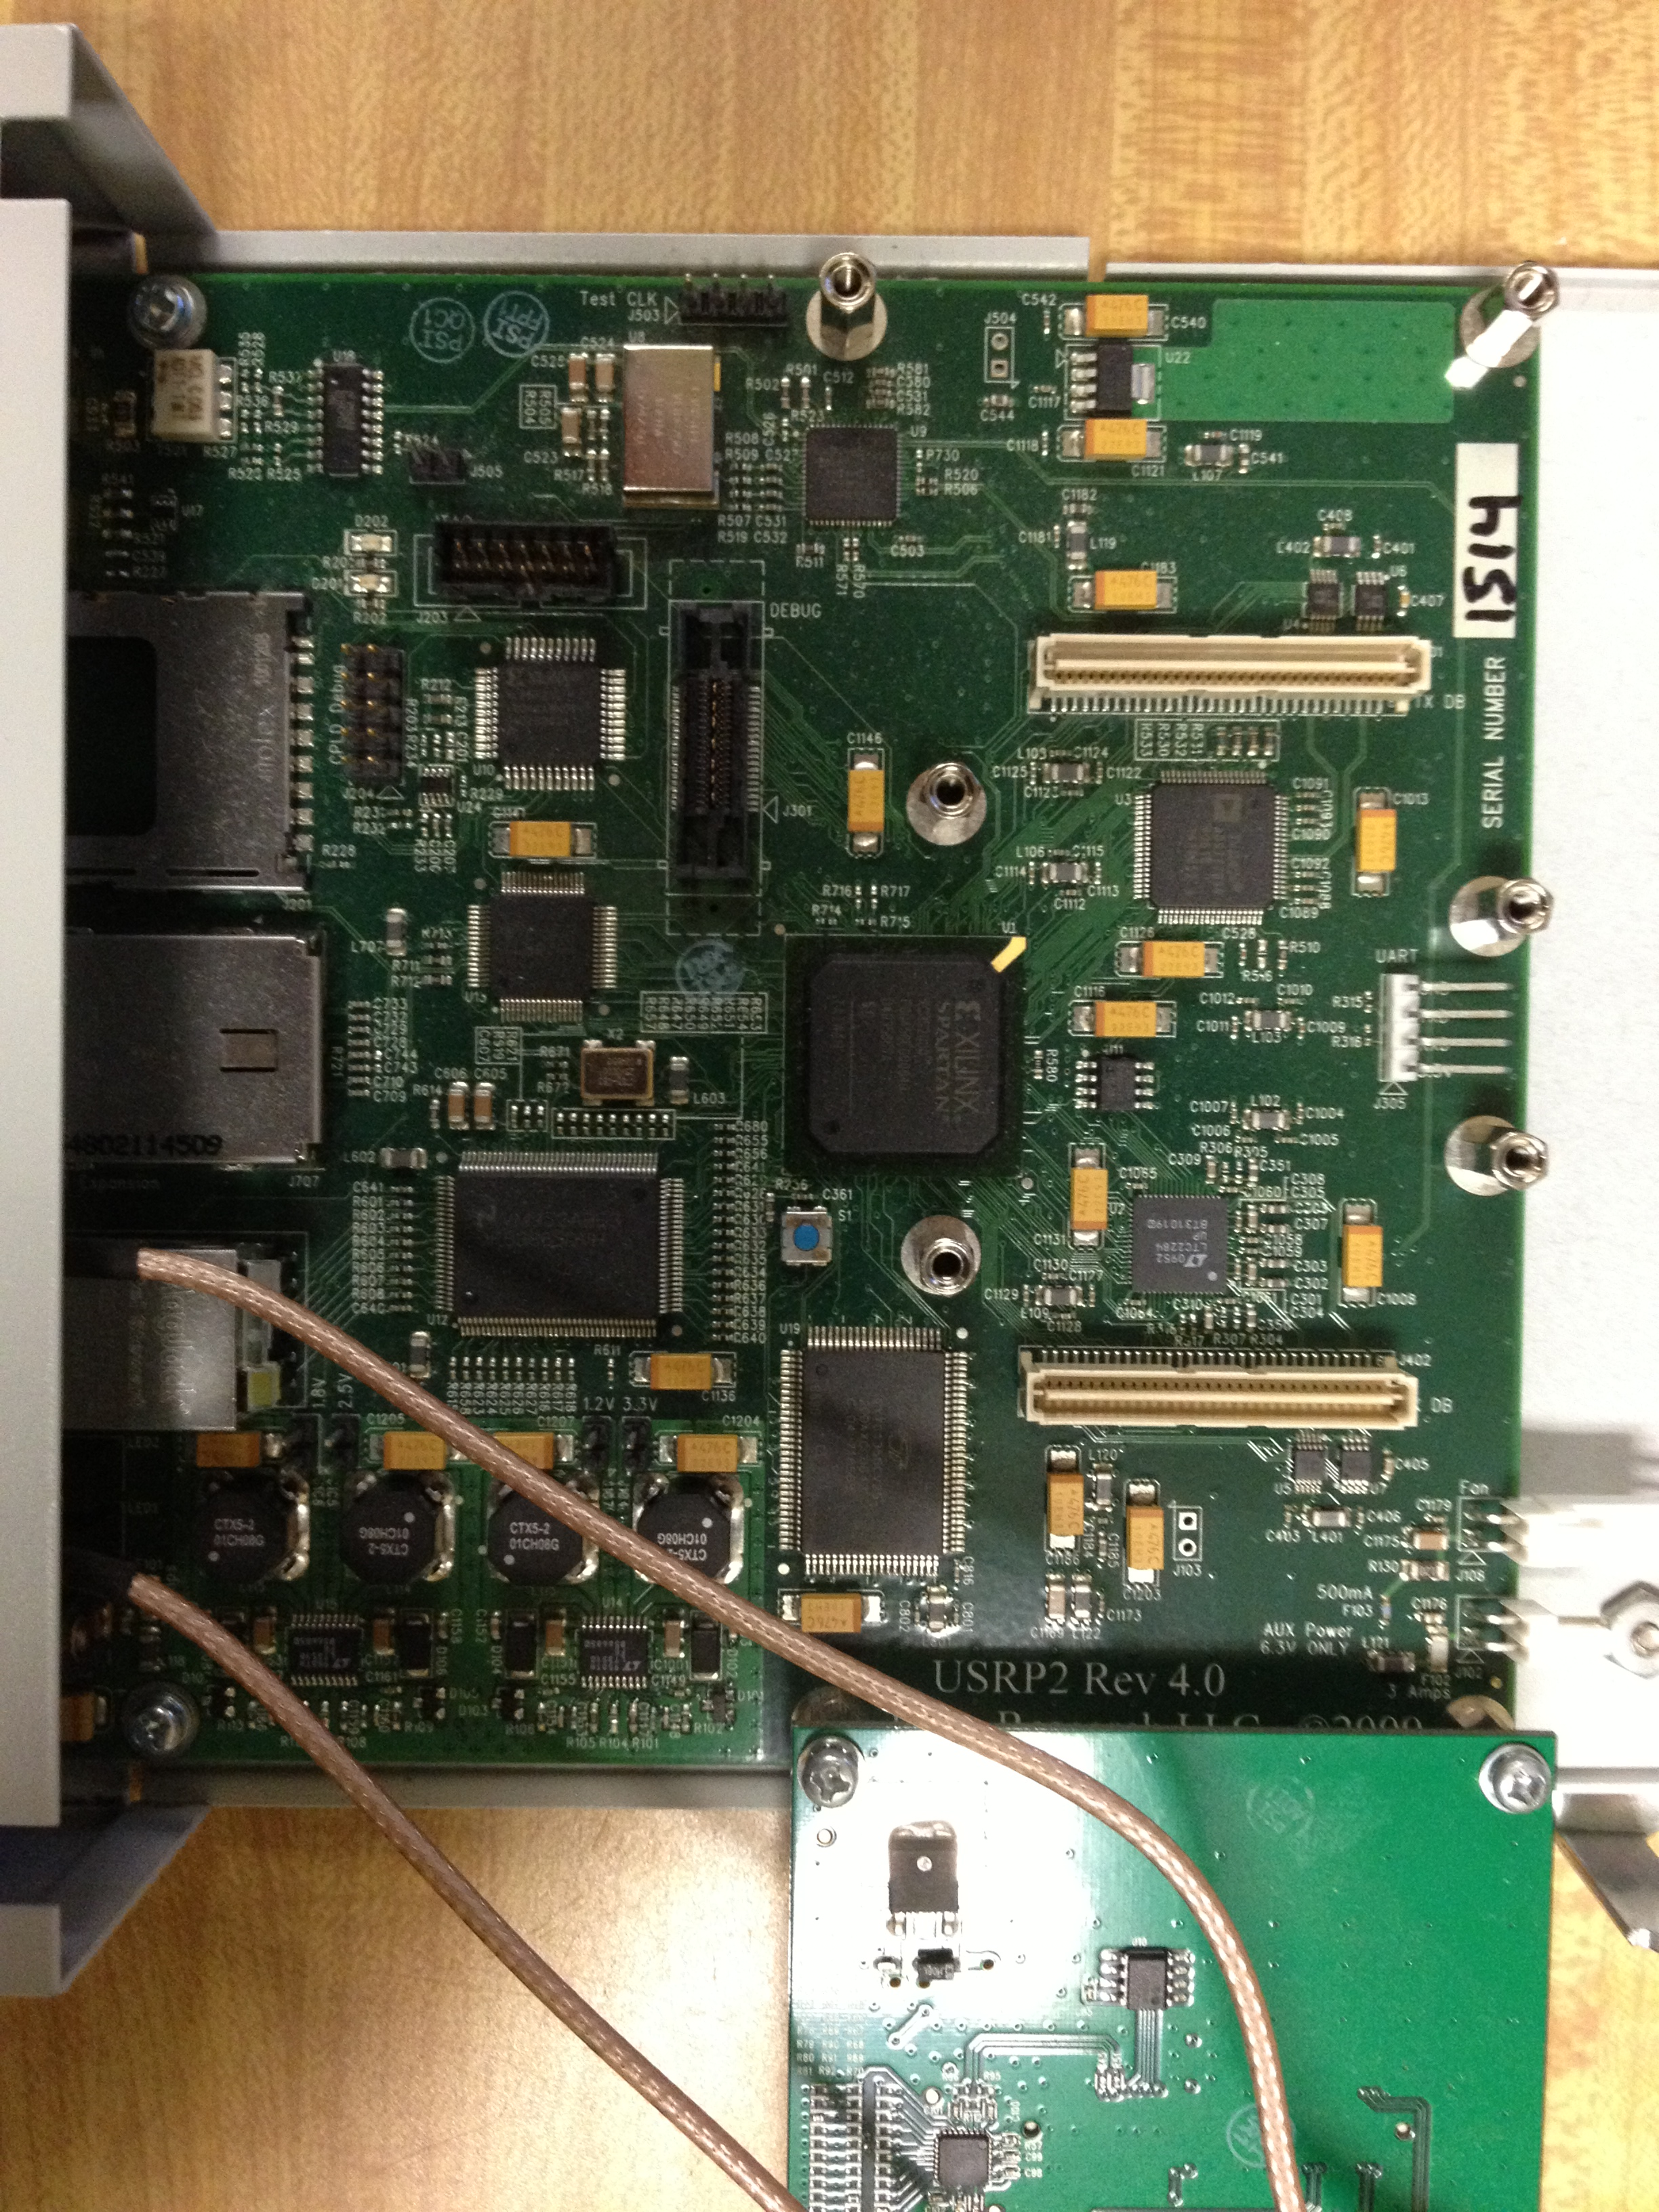
\includegraphics[scale=0.1]{usrp2_mainboard.eps}
\caption{USRP2 Mainboard}
\end{figure}


The information flow is important to understand within the phyiscal radio.  This SDR block diagram shown below, outlines the common tasks done by the: daughtercard, FPGA, DAC/ADC, and host computer.  Since the FPGA is programmable the operations can change if desire, but the three dominating software packages that utlize the USRP2 flow this structure.  Beginning on the far left of the diagram and continuing to the right, at the daughtercard are RF emitions are received and transmitted.  The daughter also contain mixers that translate the signal to an intermediate frequency.  Next come the dual 100 MS/s 14-bit ADCs, dual 400 MS/s 16-bit DACs, two digital down-converters with programmable decimation rates, and two digital up-converters with programmable interpolation rates\cite{USRP2Stats}.  These are located on the mainboard of the USRP2 itself.  The FPGA is a Xilinx Spartan 3 XC3S2000, which with the current FPGA software is 59\% free in general logic but only 3\% free in memory.  The FPGA also does not have any DSP resources.  The limited memory left in the USRP2 FPGA severely limited any additional development.  As a result on newer models, such as the N210, the FPGA has been upgrade.\cite{n210spec}\\

\begin{figure}[!ht]
\centering
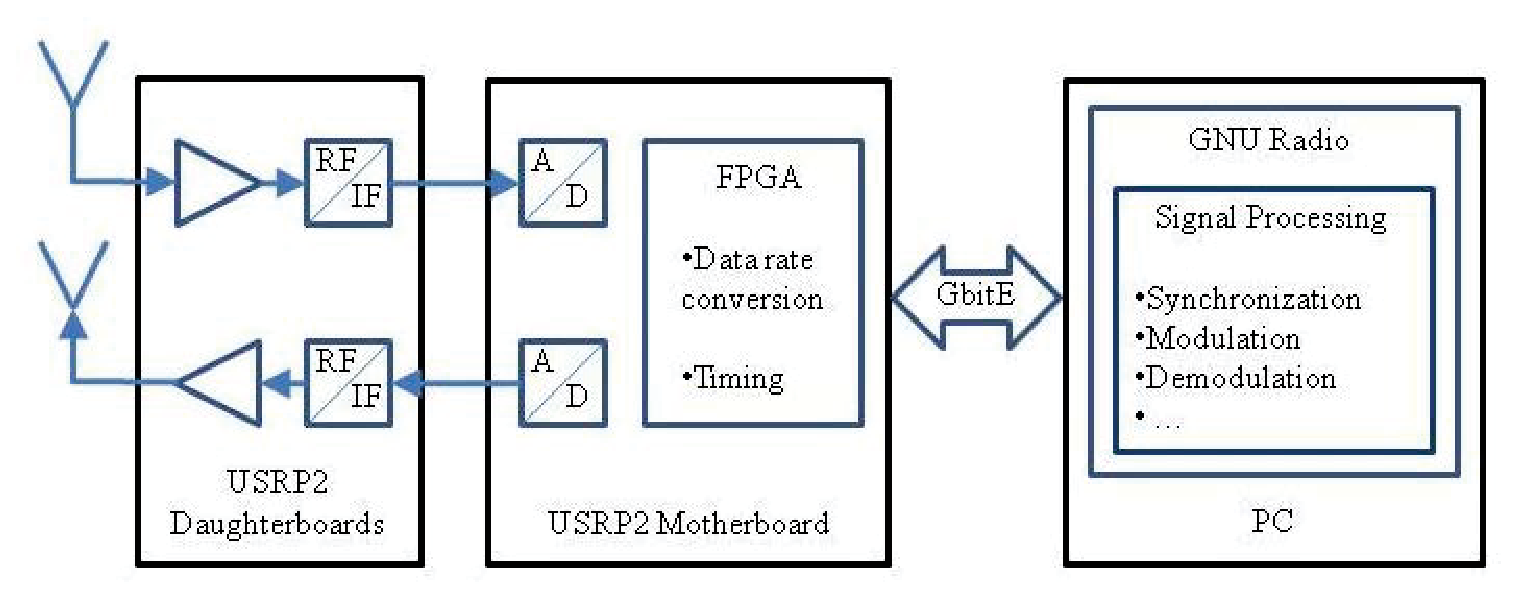
\includegraphics[scale=0.5]{sdr_block_d.eps}
\caption{USRP System Block Diagram\cite{sdr_blocks}}
\end{figure}

The data itself constain several pieces of metadata in a frame.  RX metadata structure for describing sent IF data includes time specification, fragmentation flags, burst flags, and error codes. The receive routines convert IF data headers into metadata\cite{metadata}.  Such metadata can be used to indicate the position and FPGA timestamp associated with the sample that corresponds to the start of the underlying frame. By default, existing blocks will transparently propagate any attributes contained on their input streams to their output streams. Blocks that use the attributes can query their input streams to locate all (key, value, offset) tuples in the region of the stream that they are currently working on in their “work” method. Likewise, blocks can copy, add or delete attributes on their output streams\cite{sdr_blog}.  This knowledge is extremely useful when doing multiple receive antenna arrays when alignment is necessary, or in any situation where fine timing information is required.\\

With the USRP hardware several software options are available including: GNU Radio, MATLAB, LabVIEW, and several custom packages.  MATLAB and GNU Radio have already been discussed, therefore the selection between them shall be discussed.  Since this system is a MIMO implementation signal alignment is a requirement.  MATLAB doesn't support sample alignment in a multiple USRP system.  The sample alignment is possible through either external means through an external clock or through the option choosen here the MIMO cable.  The MIMO cable, a picture of it can be seen in figure \ref{mimo}, is a standard 16-pole flatcable to connect tvrx, basic-rx or dbsrx boards.  Of this 16pin flatcable only two pins are used (io15 and ground)\cite{mimo_cable}.  An image also of the combined dual radio source block can be seen in figure \ref{mimo_grc} from GNU Radio.  With this requirement GNU Radio must be used for direct access with the USRP2.  Aswell full implementation of the systems blocks were first attempted with GNU Radio.  Fortunately, if necessary, data can be passed to MATLAB for signal processing from GNU Radio through the use of the file blocks and a script located in Appendix A.\\

\begin{figure}[!ht]\label{mimo}
\centering
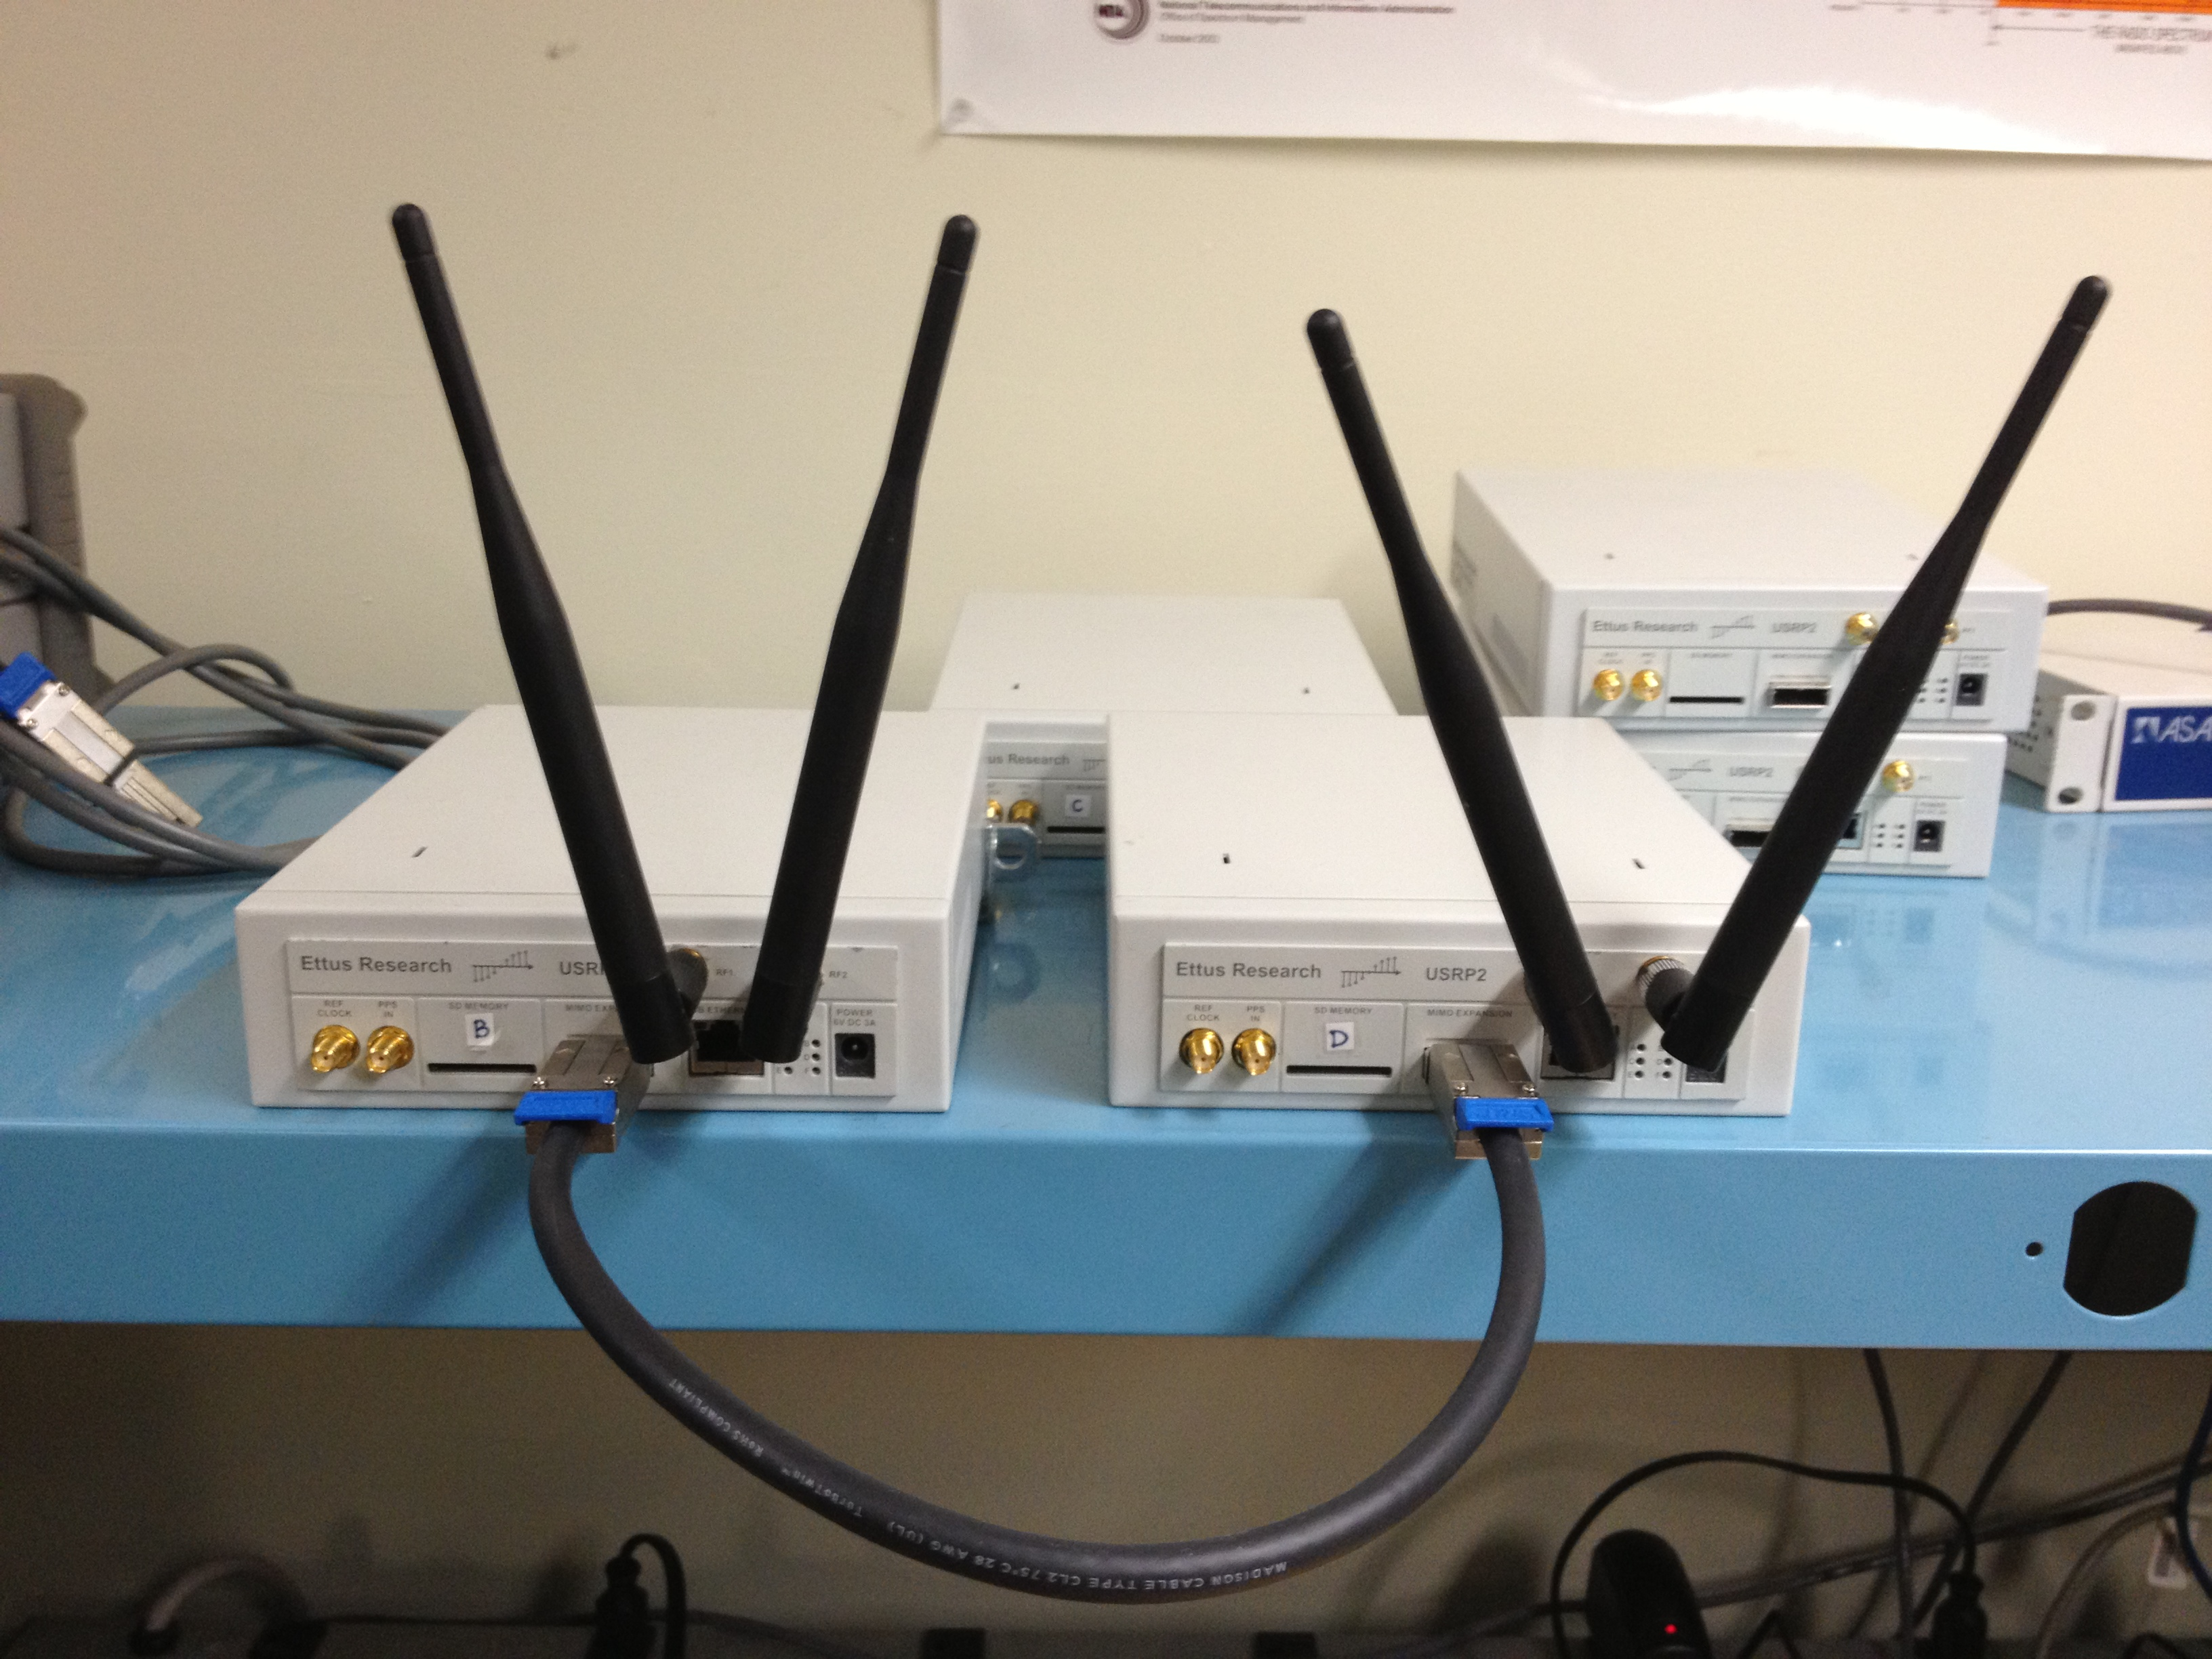
\includegraphics[scale=0.1]{mimo.eps}%taken on iphone
\caption{USRP2 MIMO Cable}
\end{figure} 

\begin{figure}[!ht]\label{mimo_grc}
\centering
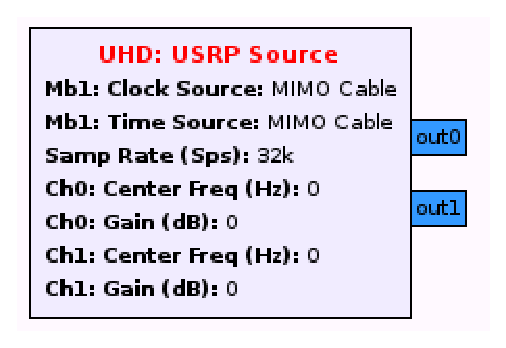
\includegraphics[scale=0.6]{mimo_grc.eps}
\caption{GNU-Radio MIMO Enable Source Block}
\end{figure} 


\section{Spectral Subtraction}

Now that the a formal system level approach has been presented and hardware setup chosen, a more detailed understanding of the blocks themselves can be examined.  The goal of the spectral subtraction block is to removal signals to allow the blind source separation block to work properly.  As discussed previously signals would first need to be identified and then removed based on information supplied in a precompiled database of known signals.  The technique to remove such signals is called spectral subtraction, which primarily takes place in the frequency domain.  This approach only relys on known PSD's of the interfering signal.  Initially this technique seemed quite sound, but futher investigation proved otherwise.\\

Initial simulations were created to examine this spectral estimation technique at RF frequencies rather than the standard audio frequencies for which Spectral Subtraction is formally used.  Only two signals were used in these simulations, both utilized the same modulation scheme and pulseshaping filters.  The signals were chosen to be non-orthoganal, since when they are orthogonal The frequency of the interfering signal was varied, and so were the oversubtraction parameter \(\alpha\) and quantization floor \(\beta\).  Through experimentation \(\alpha\) worked best at a value greater than 10, and \(\beta\) worked best between 0.05 and 0.2.  The graph in figure \ref{SS_basic} shows the bit error rate (BER) as the interferer is shifted across the wanted signal in frequency.\\

\begin{figure}\label{SS_basic}
\centering
\includegraphics[scale=0.5]{SS_basic.eps}
\caption{Original Spectral Subtraction Technique Results}
\end{figure} 

As you can see this spectral subtraction technique operates extremely poor when the signal are overlapping at all.  The reason system performs well at large frequency shifts is due to the bandpass filter which is used before the signal is quantized.  The reason the result is poor is because the estimate is largely incorrect.  Since the subtraction only utilzes the PSD's of the signals, half of the information is completely ignored.  This results in a completely inaccurate estimate.  The problem with traditional Spectral Subtraction is that its results are subjectively evaluated or done, which isn't accurate enough in a digital communication system.  Other evaluations uses such metrics as SNR, which can be quite deceptive esspecially in digital communications.  Such examples can be seen here: \cite{ss_subjective1}, \cite{ss_subjective2} \\

Since the initial simulations for traditional Spectral Subtraction proved inadiquated other optioned needed to be explored.  First though, the problem needed to be an analyzed further for better understanding, then the appropriate solution could be formulated.  Since the interfering signal and the wanted signal are non-orthoganal to one another they will share dimensional space, in this case the signals are inphase with one another.  Therefore both planes real and imaginary must be considered.  Non-orthoganal signal removal is a common task in communication system, which is done primarily by equalizers.  Therefore an equalizer approach was considered next.\\

\subsection{Equalizer Approach}

The equalizer approach used in this Spectral Subtraction approach is a Least Means Square (LMS) equalizer, utilizing training data used in the front portion of each transmitted frame.  This a common equalizer used in practice, allowing for future translation into a realized implementation.  The LMS equalizer was also chosen for it robustness no noise, which is a weakness of such equalizers as the zero-forcing equalizer and requires no matrix inversion such as the Least Square (LS) equalizer.  For proof of concept the entire datastream is used as training data, which provides the best results of any given channel for an adaptive equalizer, since the maximum knowledge is gained about the channel for each frame received.  The results below show the BER as the signals pass over one another in frequency, similar to the previous evaluation using traditional Spectral Subtraction.\\
  
\begin{figure}[!ht]\label{SS_equalizer}
\centering
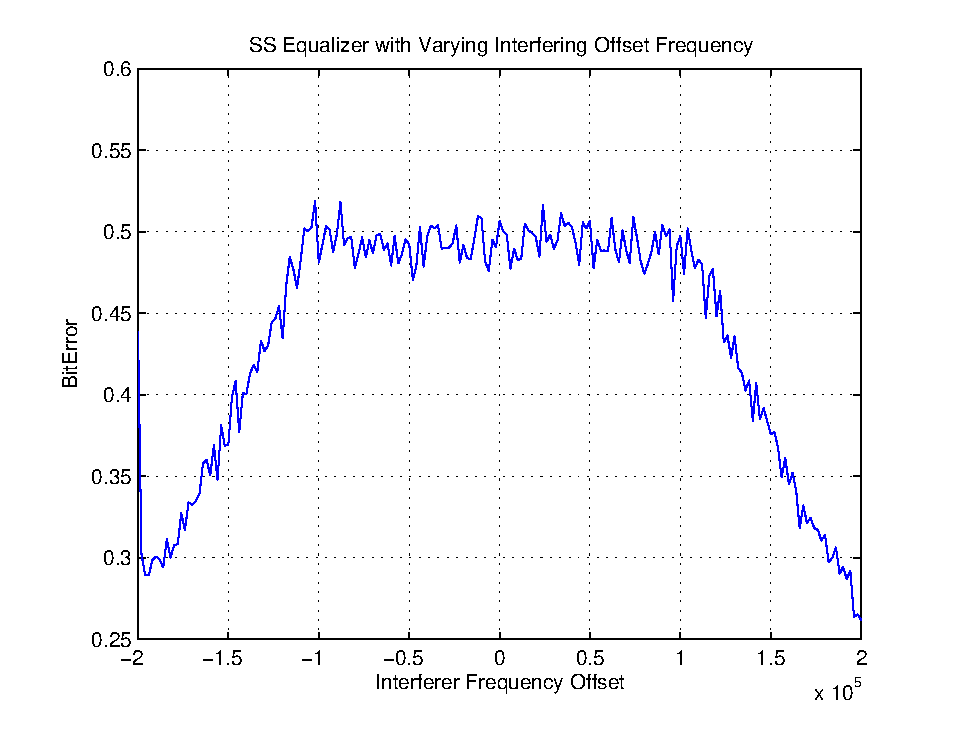
\includegraphics[scale=0.5]{SS_Equalizer_sim.eps}
\caption{Spectral Subtraction Equalizer Test}
\end{figure} 

As you can see the figure above, the equalizer approach doesn't provide any improve beyond the traditional Spectral Subtraction approach.  The problem with using traditional adaptive equalizers is that they can only be used with a comparative slowly fading channel.  Since knowledge learned from the training data can be applied at the earliest to the next frame, if the interference changes enough it can render the equalizer useless.  This rapidly changing spectrum or energy within the spectrum is unforunately a common characteristic of jammers.  Even though this approach failed it provided an important observation and incite into the requirements and scenarios in which jammers can be overcome.  For the sake of completeness an additional test was done with a small repeating sequence, smaller than the equalizer tap size, and as aspected the equalizer was able to overcome the interferer.\\

%\begin{figure}\label{SS_equalizer_small}
%\includegraphics{SS_Equalizer_small.eps}
%\end{figure} 


The important conclusion drawn from the previous experiment is that the when signals are orthogonal the receiver needs to be able to predict what data or energy is being transmismitted at a given time.  Therefore the jammer problem must be constained future.  As a result two jammer scenarios will be defined.  The first scenarios is that the jammer's modulated data or energy is completely known to the receiver and the second is that the data sequence repeats with period being small.  The larger the period the more resources the receiver will need to devote to its determination and evaluation.  The sequence being completely known to the jammer is a reasonable assumption; primarily if the jammer is friendly, as discussed previously in this thesis, then that knowledge can be readily available.\\

Now that the jammer scenarios have been defined further they can be evaluated.  The first will be when the data sequence of the jammer is completely known to the receiver.  The approach here will be to synchronize with the interfering signal, so the interferer will simply be subtracted off.  To synchronize the signals a mathematical tool called correlation will be used.  Correlation is a common tool used in synchronization in communication systems when looking for known symbols in a stream of data.  Equation \ref{cross} for cross-correlation simply passes signals over one another, the resulting sequence creates peaks where the data is most correlated.\\

%\[ (f\star g)[n] = summation f^{\star}[m]g[n+m]\] NEED CITATION\\
\begin{equation}\label{cross}
R_{XY}(t_{1},t_{2})=E[X_{t_{1}}Y_{t_{2}}] \cite{gubner}
\end{equation}

An example of two sequences being cross-correlated with one another can be seen below, with the peak being where the signal line up of share the most mutual information with one another.  Therefore from this data the location of the start of the interfers data can easily be located and removed.  A simulation was created with this design in mind, with a unique result.  Since the signals are frequency shifted over one another, when there frequencies match, it produces the best result, but as soon as they are offset, errors start to occur.  This can easily be compensated for using a complex exponential multiplied by either the received or catalogued waveform.  This will enduce a frequency shift cancelling out the shifting signal.  Therefore the error is just a function of the noise itself.\\

\begin{figure}[!ht]\label{ss_correlation}
%changing power graph of subtraction
\centering
\includegraphics[scale=0.5]{ss_correlation_sim.eps}
\caption{Spectral Subtraction Correlation method}
\end{figure} 

This simulation was also repeated but this time was subtracted in the frequency domain.  The result produced near identical results.  Since using this approach requires two fourier transforms, into and out of the frequency domain, computationally it is much more involved and requires many more resources than the time domain approach.  If the data was already the frequency domain from some other process or signal processing technique then the frequency subtraction would be a viable option.\\

Further analysis was done to provide a solid understand of the new requirements of the system and its limitations.  The first is the precise understanding of the interfering signal itself.  Since it is assumed that the signal modulation and data stream is known, attention can be shifted to the other issues that can occur, which are the non-idealities of the system.  The first is the power constraint or effect.  When subtracting the interferer specific power must be measure of the interferer alone, so close to as little possible energy is subtracted from the joined signal that belongs to the desired signal.  An examination of the incorrect estimation of the interfering signal was examined in \ref{power_delta}.

\begin{figure}[!ht]\label{power_delta}  
%changing power graph of subtraction
\centering
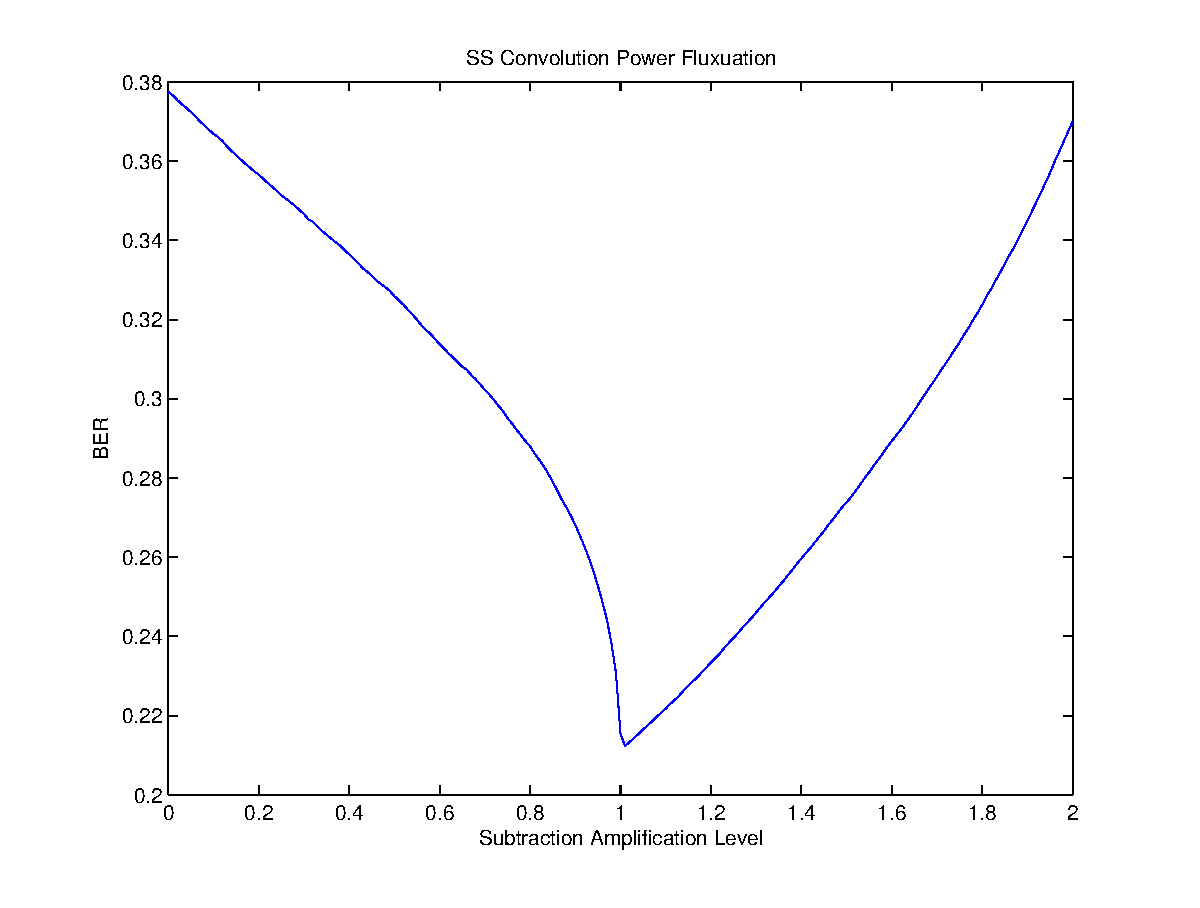
\includegraphics[scale=0.5]{ss_conv_changing_over_subtraction_level.eps}
\caption{Spectral Subtraction Correlation Test with Varying Oversubtraction Level}
\end{figure}

Besides power, frequency and timing offsets were examined.  These are especially concerning because the signal cannot be demodulated when in operation for feedback information, because it must be fed into the signal separation block for equalization.  Therefore a timing recovery mechanism cannot downsample the signal either.  The timing recovery and carrier recovery mechanism therefore needed to be unobtrusive as possible to the signal.  As a result frequency and timing shifts were examined to understand the sensitivity of the subtraction, and how accurate the recovery mechanismed needed to be.

%Freq Shifting
\begin{figure}[!ht]\label{shifting}
%Timing (Phase) shifting
\centering
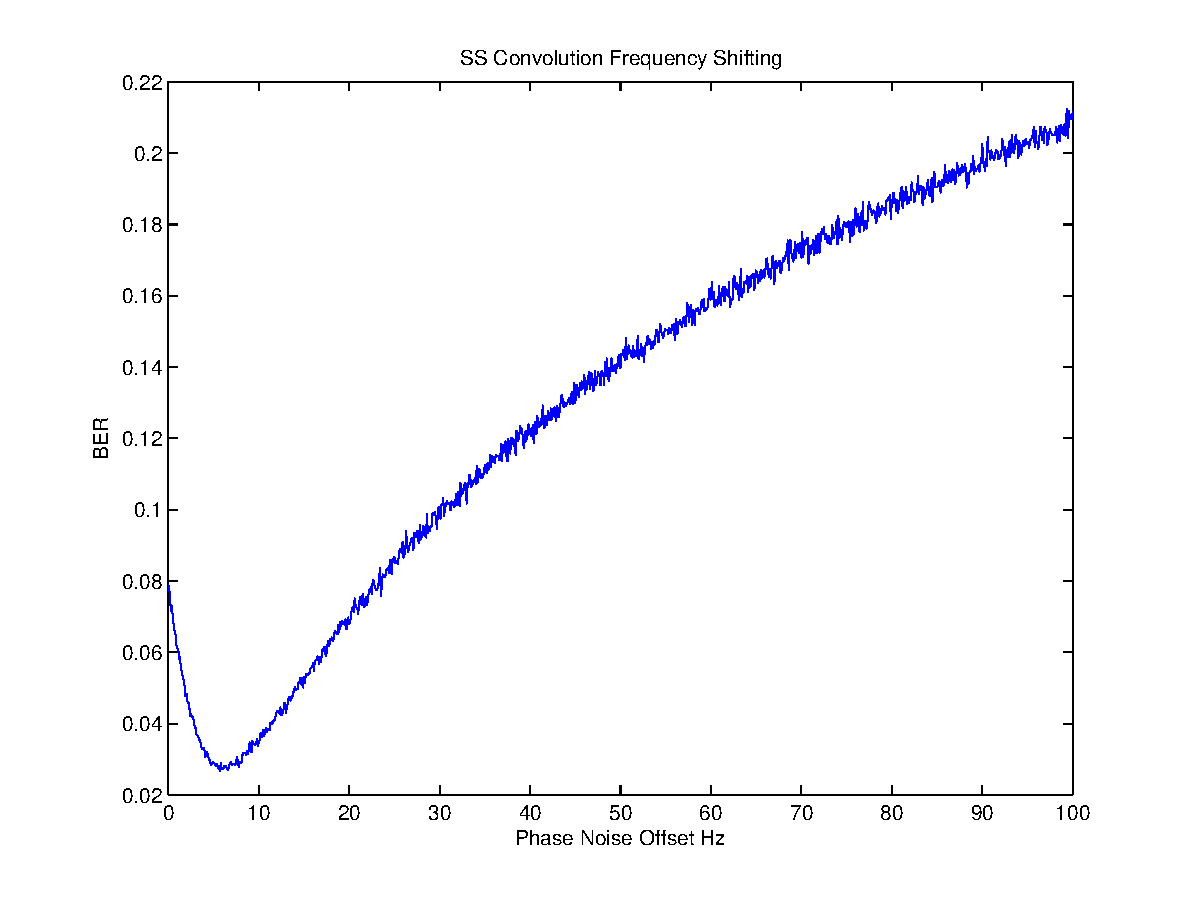
\includegraphics[scale=0.5]{ss_conv_phase_offsets.eps}
\caption{Spectral Subtraction with Phase Offsets of Interfering Signal}
\end{figure}

As you can see from figure \ref{shifting}, the subtraction mechanism is extremely sensitive to timing offsets, while frequency shifts the system is rather robust.  If a full bitshift occures though, the entire system falls apart.  This is a rather large problem and must be considered when attempting such operation on non-simulated data.  This problem was forsean because of the time variance or sensitive of the signals themselves. \\

Moving on, now that a viable subtraction technique has been determined, the final implementation for the Spectral Subtraction block can be realized.  As discussed in the Hardware and Software Platform section of this thesis, GNU Radio was the first to be examined because of its realtime attributes.  This was quite an involved process requiring many weeks of trial and error.  The first implementation was entirely written in C++, which is the recommended language for signal processing blocks in GNU Radio.\\  

Since C++ within GNU differs from many modern programming styles a code implementation or route was taken to ensure accuracy and speed up development.  Therefore all coding was done with C++ itself, using no GNU Radio built-in libraries\cite{gnuradioCPP}.  To allow for matrix operations the Aramdillo C++ Library\cite{armadillo} was imported and provided needed vector operations such as correlation and faster mathematical functions instead of having to rewrite common search operations.  This library would also be needed for the Signal Separation block, therefore coding with Armadillo would provide the knowledge for future implementations needed in that block.  From the standard C++ implementation results were compared with Matlab, and the code was ported into GNU Radio.\\

\begin{figure}[!ht] 
\centering
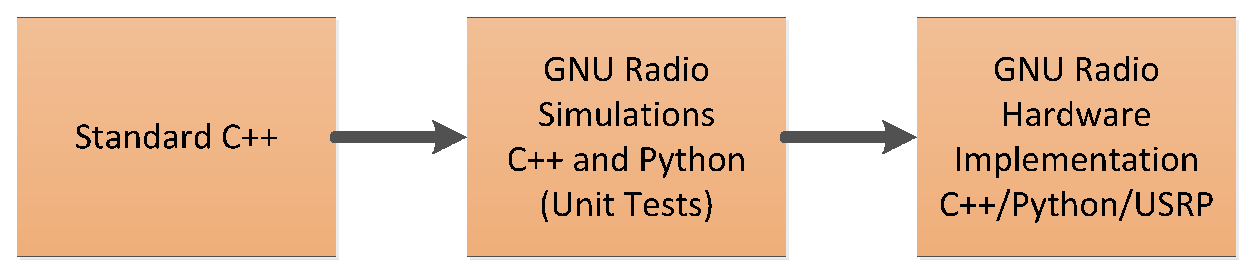
\includegraphics[scale=0.5]{code_work_flow.eps}
\caption{GNU-Radio Code Implementation Workflow}
\end{figure}

GNU Radio C++ are basically written by first creating test cases and writing your code until they are solved.  This is a common practice among the programming community and provides a definitive endpoint to the code itself.  The code was written and compiled successfully but unforunately the python wrapper called SWIG\cite{swig}, which GNU Radio uses to interact with the C++ block through python, was unable to export the library.  This is an undocumented problem within GNU Radio and was only identified through discussions directly with the GNU Radio core development team.  Therefore another approach had to be considered.\\

The next option was to use python itself for signal processing.  This is approach was primarily developed by Josh Blum, one of the core developer of GNU Radio.  It isn't recommended due to speed issue, but it is quite easier to implement and debug for those familiar with python.  As a result the previously C++ code was ported to python standards libraries and then to GNU Radio.  The NumPy libraries were used within python.  NumPy is the fundimental package for scientific computing in Python\cite{numpy}.  It like the armadillo library provides matrix operations such as correlation.  Again under the Python standard libraries with NumPy the results were varified with MATLAB.  Then the code was port to GNU Radio.\\

Again more problems occured, stonewalling all progress.  The signal processing block was written as a subprocess using the queuing system built into GNU Radio.  Queueing provides barriers between the connected blocks; therefore they can run freely, limiting bottlenecks. The system built would operate correctly for several hundred samples but would eventually segmentation fault.  Several attempts to fix this error with even architectural changes to the code.  Finally the lead developer of GNU Radio was consulted, Tom Rondeau \cite{tomrondeau}, but he was also unable to determine a solution.  The assumed problem was a type casting occuring within the queue itself, that would eventually accumulate and cause a segmentation fault.\\

With these setbacks, it became necessary to look beyond GNU Radio and just utilize MATLAB for signal processing.  Therefore the decision to load captured signals from GNU Radio and process them in MATLAB.  It is nowhere near realtime, but it will process the data appropriately.  The simple GNU Radio needs frontend is important because it allows tight synchronization between multiple receive antenna, which is a require of the original design of the system.  The GNU Radio model can be seen in figure \ref{grc_receiver}, the modulator block has been customized to remove the quantization, producing floating point results.\\

\begin{figure}[!ht]\label{grc_receiver}
\centering
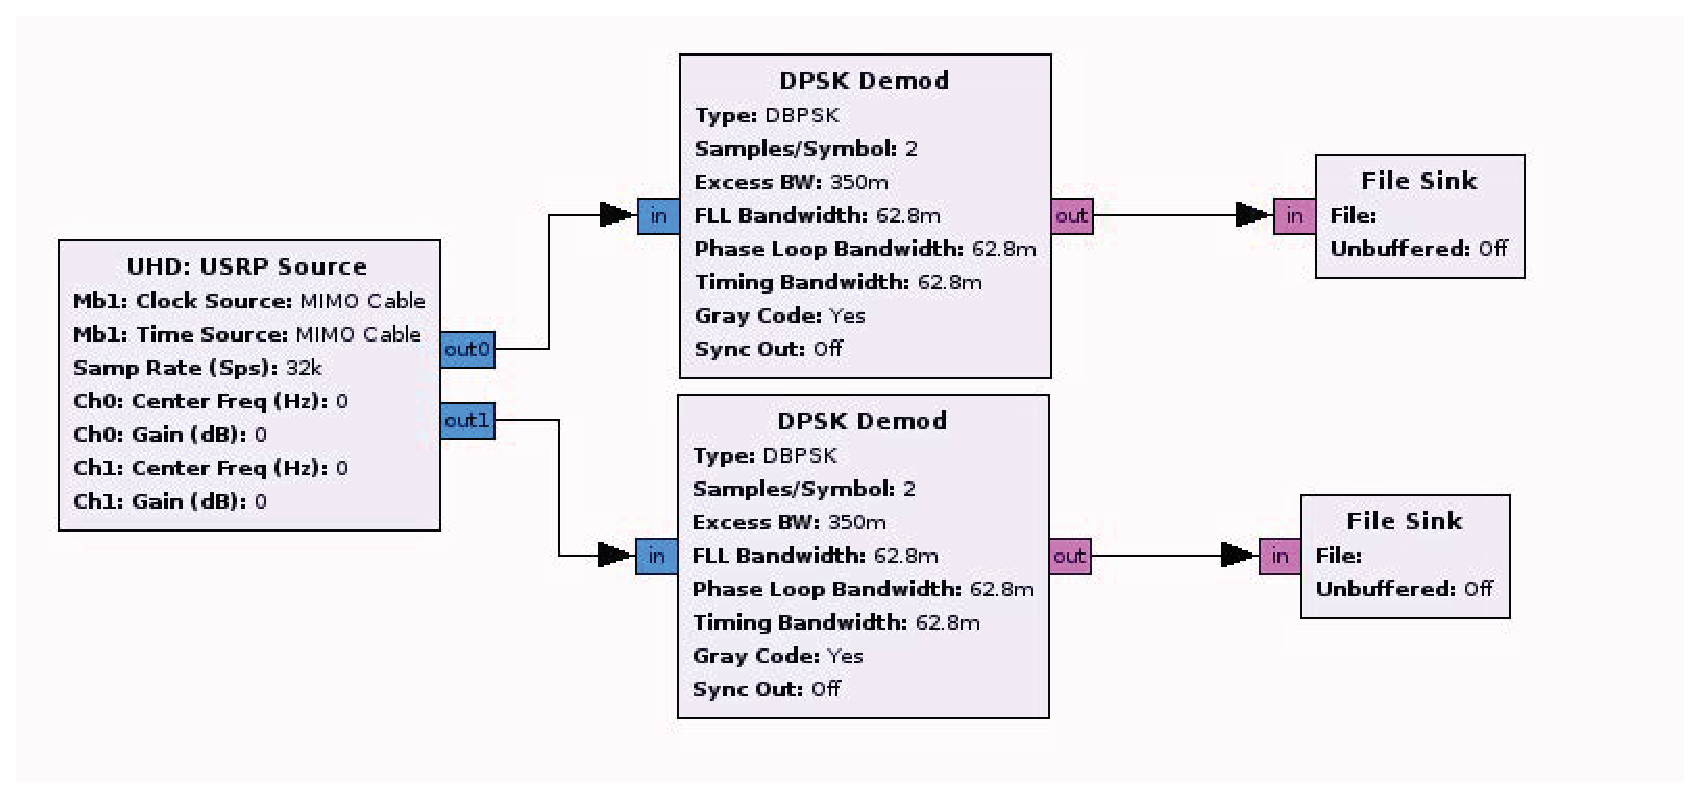
\includegraphics[scale=0.5]{grc_receiver.eps}
\caption{GNU-Radio Receiver Half Design}
\end{figure}

\subsection{Non-deterministic Scenarios}

For completeness it is important to discuss the scenarios when the interferer's modulated data is unknown but repetative with a small period.  The approach to estimating short sequences is a rather obvious one, an autoregressive algorithm is used to predict samples.  The simulation here, which was just used for proof of concept, uses a linear predictive filter.  The filter determines coefficients of a forward linear predictor by minimizing the prediction error in the least squares sense\cite{lpcfilter}.  It finds the coefficients of a pth-order linear predictor (FIR filter) that predicts the current value of the real-valued time series x based on past samples.

\[ \hat{x}[n]=-a(2)x(n-1)-a(3)x(n-2)-...-a(p+1)x(n-p)\]

For the linear predictive filter to operate efficently the number of filter taps must be equal to or greater than the period of the repeated sequence.  If the number of taps is smaller it cannot capture the randomness the in the interferer's data.\\

\subsection{Over the Air Implementation Considerations}

When moving towards a real implementation of the Spectral Subtraction block, the non-idealities introduced by the envirorment needed to be considered.  These include frequency and phase shifts, as well as timing offsets.  Certain considerations needed to be made as well, since instanteous changes occur when signals overlap.  Therefore a more advanced control scheme needed to be constructed around the common signal compensation or correction.  The basic idea used here is a receiver within a receiver, one for each signal received.  This will be discussed in detail.\\

The system assumes that the jammer is always present within the envirorment therefore it was concluded that the jamming signal should be synchronized with first, be removed and then all that remains should be the wanted signal.  There is were the receiver within a receiver design comes in, since first the interferer will be synchronized to, utilizing phase and frequency recovery and then timing recovery.  Unforunately such an implementation isn't as straight forward as expected.  Since when both signal are present in the spectrum it is impossible for these algorithm to operate correctly.  This is due the fact that they cannot separate one signal from the other.  For example, phase information cannot be accurately calcuated in the presence of two signals.  Therefore modifications need to made, which is where a controlling mechanism comes into play.\\

When multiple signals are in the envirorment the compensation algorithm learn incorrectly; as a result, a decision was made to pause these algorithms when both signals were present and continue when the signal interferer was only present.  This operation relys on two assumptions, the first is that both signals are present for short periods of time which can be controlled.  The second is that the calculated offsets of cause by the envirorment don't rapidly vary during the periods of time for which the two signals are visible.  This assumption is quite reasonable especially with relatively non-mobile transceivers, which was assumed in the original documentation.\\

To accomplish this algorithm holding mechanism, energy detection was chosen to be uses for its simplicity.  Below you can see an image of the jammer signal by itself and the combined signals.  A large increase in energy or step can be seen, which can easily numerically detected.  Energy is calculated using the following equation: \(E_{s}=\newcommand{\inftyint}{\int_{-\infty}^{+\infty}}|x(t)|^{2}dt\).  This was implemented with a moving average filter with a small window to reduce sperious changes due to signals gaps or outliers.  In practice the average peak energy level of the interferer is first calculated, then when the power in the spectrum increases to a level roughly 1.5x of the original level, the compensation algorithms are halted.  A simple technqiue technique, which is commonly uses but in the inverse fashion.  An example of the combined and signals can be seen in figure \ref{combo_signal_time}.  The final results of the Spectral Subtraction block are examined in the next chapter.\\


\begin{figure}[!ht]\label{combo_signal_time}
\centering
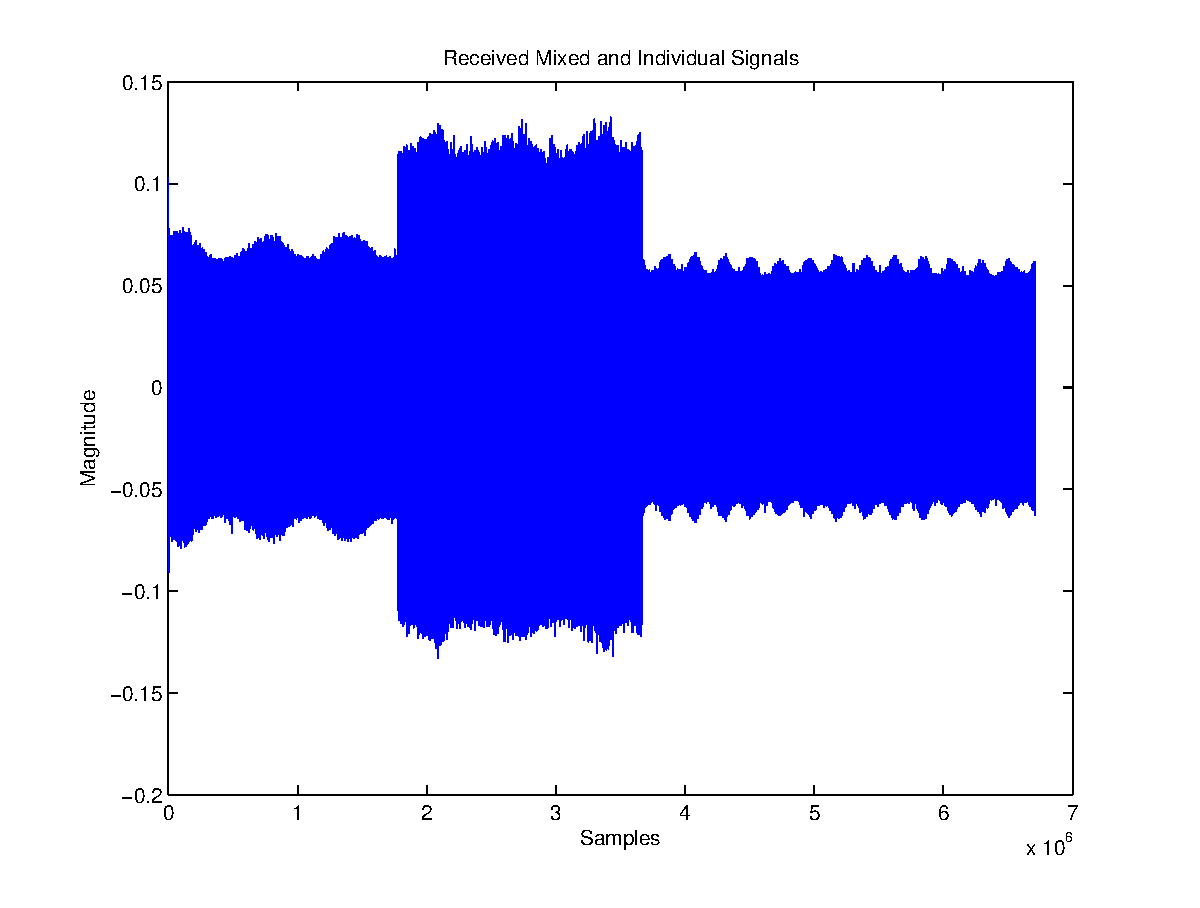
\includegraphics[scale=0.5]{combo_signal_time.eps}
\caption{Received mixed and individual signals}
\end{figure}

\section{Superimposed Equalizer}

Moving on, the next block to discuss is the signal separation block.  The development of this block is very staggered and due to time requirements shortcuts needed to be made.  The original desired result was to use a blind source separation technique outlined here \cite{AMUSE}, which is able to separate multiple signals from one another under specific constraints.  For this process to work efficently an appropriate channel model needs to be created.  Since the goal of this system is to be very robust an estimator for very frequency selective channel is desired.  The progession of the signal separation block will be examined in this sections and the limitations will be discussed.  It is important to note that a large variation was taken in the system design due to implementation feasibility.\\

The original objective was the utilize a new signal separation technique called AMUSE, but a new avenue was taken with a more theoretical channel estimation problem in mind.  This estimation evaluation will be discussed first.  The first objective for channel estimation is to examine the channel mixing model which assumes a single-input multiple-antenna broadcast channel.  A J-channel FIR system excited by K transmit antennas is considered. A quasi time-invariant multipath channel is assumed which remains constant during the transmission of a set of consecutive symbols, which are called slots. These slots are assumed independent from one another.  The channel estimation is performed over each slot. Each symbol inside a slot is assumed to be the result of a known redundant precoder acting on an input transmit symbol vector drawn from an M-PSK constellation. Therefore the receiver receives signals not only from the intended transmitter but also from Q other interferers. The interferers are assumed to employ the same redundant precoder as the desired signal\cite{skrkantPHD}.\\

With this model, \cite{midterm_report} shows that no assumptions are necessary regarding the number of the transmit antennas of each of the interferers and the channel orders as long as they are smaller than the block size.  The block size in this case is equal to the combination of the individual channel lengths and the number of transmit antenna used by the desired transmitter.  But this evaluation rely on three assumptions:

\begin{enumerate}
\item The data sequence \(x_{d}\) is an i.i.d. sequence such that \(x_{d}\sim\mathcal{CN}(0,\sigma_{d}^{2})\)

\item The distribution over the MIMO channel vector is \(p(y;\theta)\sim\mathcal{CN}(\mu_{y},R_{w})\), and the interference vector is distrbuted normal with covariance \(R_{w}\)

\item The transmitted symbols, the channel vector, and the interference vector are jointly independent
\end{enumerate}

With these assumptions the mixing process can be undone but the channel estimation needs to be calculated first.  Since this is a MIMO channel, frequency selective fading will need to be captured to providing appropriate channel knowledge.  To accomplish this, the original research decided to utlize superimposed equalization, whose operation was heavily discussed in the background section of this thesis.  In summary, \cite{Ghogho} uses a superimposed symbol transmission scheme to estimate frequency-selective channels. Several points of the DFT of the data are set to known values. This operation can be easily implemented in the time domain when these DFT points are equispaced. The channel is estimated using the DFT of the received signal at these selected DFT points. The detection itself is done using an iterative method across these points.  Unlike traditional equalizers, the proposed method does not require bandwidth for training.  It instead trades spectral power for those symbols themselves, spreading its energy over the entire bandwidth capturing the entire spectrum space.   \cite{Ghogho} also proves that by placing the training symbols in quasi-periodic position they will not interfer with the data itself.  It is important to note that this research discusses no sychronization mechanism, and now with the training data spread throughout the signal is very complex.  This addition complexity was factored into the design decisions of the implementation, which is discussed later in this section.\\

With our channel estimation method chosen, a simulation was created to prove the effectiveness of such a scheme.  The result of this implementation were directly compared with the results of the paper to prove correctness.% and compared with traditional equalizer performance&
The results of this simulation are seen in figure \ref{sie}.  It examines a random frequency selective channel, with very high suppression with a across a number of SNR values.  As expected there is a linear relationship between SNR and Error.\\  %For completeness a comparision was done with a traditional LMS equalizer to show the effectiveness of the superimpose equalizer.\\

\begin{figure}[!ht]\label{sie}
\centering
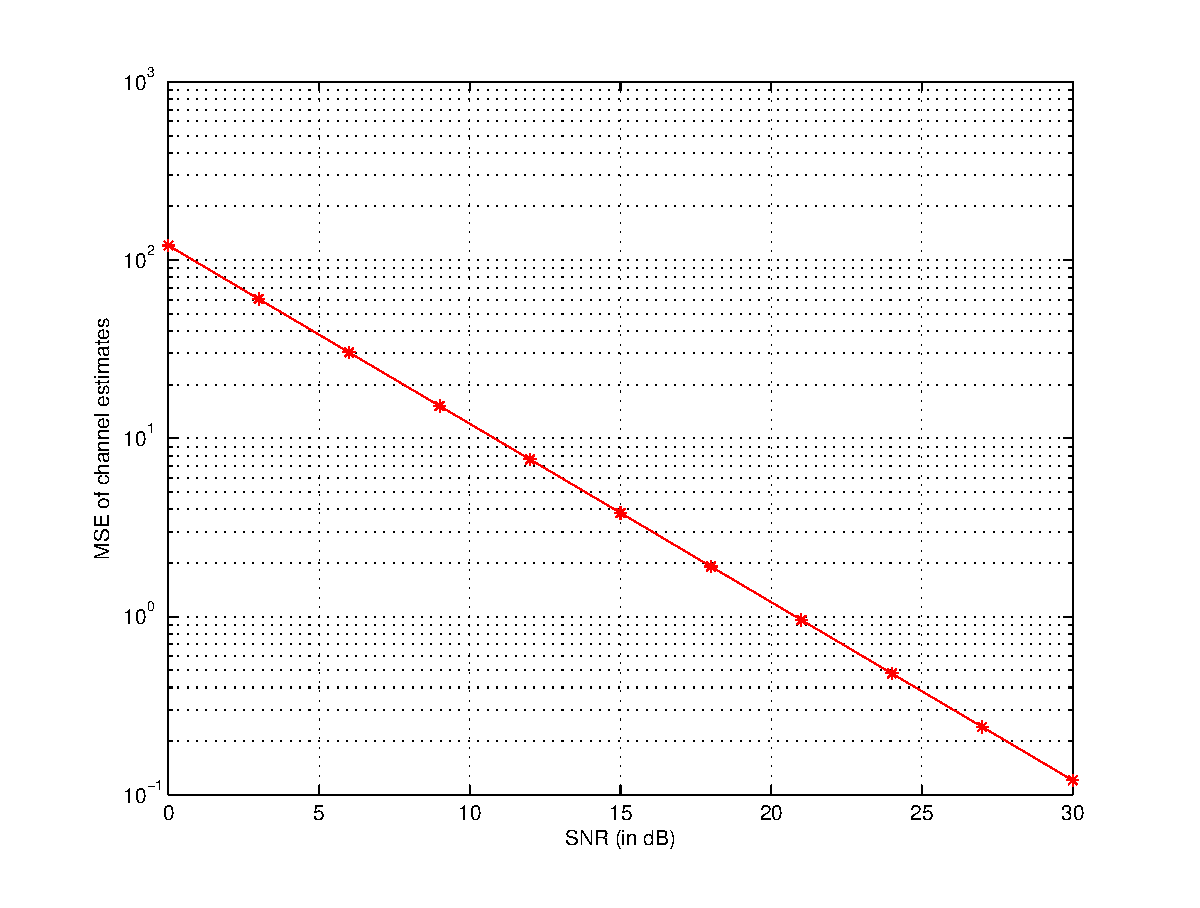
\includegraphics[scale=0.5]{sie_SNR.eps}
\caption{Superimposed Equalizer SNR Performance}
\end{figure}

\begin{figure}[!ht]\label{sie_freq}
\centering
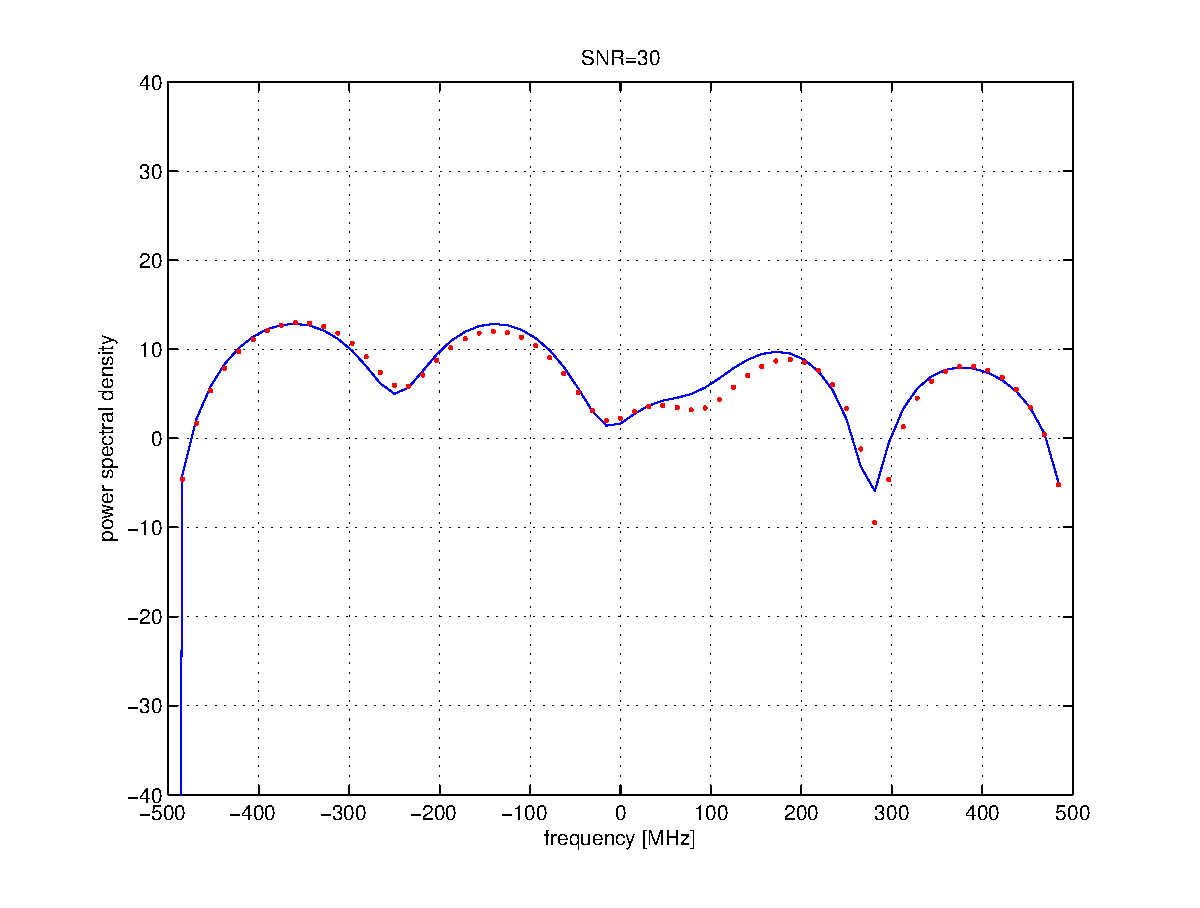
\includegraphics[scale=0.5]{freq_response_sie.eps}
\caption{Superimposed Equalizer Channel Estimation Performance with High SNR}
\end{figure}

%INSERT Figure of SNR and channel estimate for Superimpose equalizer\\
%
%INSERT Figure with comparision of superimposed equalizer vs. traditional linear equalizer\\

From figure \ref{sie_freq} you can see in a frequency selective fading channel is very well estimated by the superimposed equalizer.  This was exactly the result that was desired, but symbol recovery after equalization still needed to be examined. This unfortunately is the drawback of this formulation.  The first is the condition if the mixing matrix \(H\) is rank deficient, the channel become inestimiable,  since there become an infinite amount of solutions to the actual unmixing process.  The second is the equalizer, which is numerically intensive, and the alternative has limiting conditions \cite{Ghogho}.  This conclusion, which isn't discussed in \cite{Ghogho}, is when the equalized signal is very suppressed due to the incomplete channel estimate.  The quantization feedback method overcome the previously received frame and dominated all future frames, essentually neglecting any information they have.  Again this only in very suppresive channels.  With these results the superimposed equalizer started to become less desirable due to it's complexity, but evaluations continued due to the amount of time invested into the topic already.\\

%NEED MORE MATHEMATICAL EXPLAINATION 


%%%%%%%%%%CONTINUE EDITING
%%%%%%%%%%CONTINUE EDITING
%%%%%%%%%%CONTINUE EDITING

These simulations provide the necessary foundation to push towards the final implementation of the signal separation block.  However, due to time constraints certain decisions needed to be made about this block and the feasibility of its operation.  With that in mind the primary goal for the signal separation block was to provide signal separation or maximization from several received signals.  Since the previous research provided substantial implemenation considerations and issue, a new direction needed to be considered.  Therefore instead of the proposed AMUSE\cite{AMUSE} technique, another MIMO cross-channel technique called Maxmimal Ratio Combining (MRC) was chosen as a viable alternative.  This decision was made with both project managers.\\

Maximal Ratio Combining is a method of diversity combining in which the signal add first weighted and then added together.  These weights or gains are made proportional to the RMS signal level and are inversely proportional to the mean square noise level in that channel, and the same proportionality constant is used for all channels\cite{fs1037c}.  Therefore the channel with the best SNR provides the greatest impact on the resulting sequence.  This process needs to explain more throughly.  Assuming the received signal is an array of samples received the individual antennas \(\boldsymbol{x}(t)=\boldsymbol{h}(t)u(t)+\boldsymbol{n}(t)\) and the individual channels \(\boldsymbol{h}=[h_{0},h_{1},...,h_{N-1}]^{T}\), and the additive noise \(\boldsymbol{n}=[n_{0},n_{1},...,n_{N-1}^{T}\).  The equalized symbol \(\hat{x}=x+(h^{H}n)/(h^{H}h) \) \cite{diversity}.

A simple evaluation of MRC was done to prove its capabilities, which is based on the simulations here \cite{mrc_m}.

\begin{figure}[!ht] 
\centering
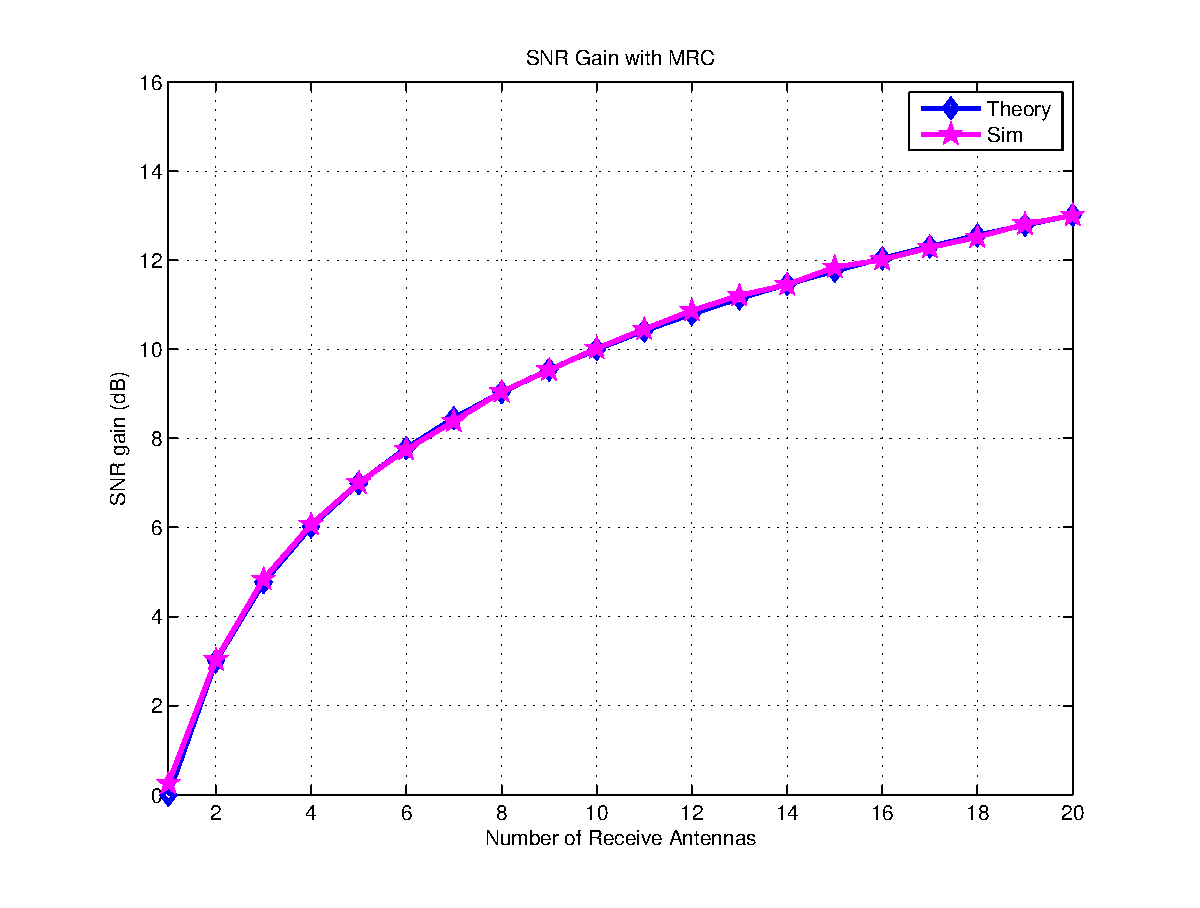
\includegraphics[scale=0.5]{mrc_gain.eps}
\caption{Maximal Ratio Combining gain acrossing varying number of antennas}
\end{figure}

As you can see as you increase the number of antennas in a frequency selective channel the better the result.  Therefore MRC was introduce into the framework of the signal separation block, and the new model for this block can be seen in figure \ref{mrc_sys}.  This block first utlizes adaptive equalizers on the channels individually then uses MRC to combine there results maximizing the SNR of the desired signal.  MRC was combined with the channel estimate approach using adaptive equalizers due to there known feasibility.  From the knowledge learned in the previous with the implementation involving GNU Radio, the signal separation block was created entirely in MATLAB.  The results of this operation will be discussed in the final chapter of the thesis.\\

\begin{figure}[!ht]\label{mrc_sys}
\centering
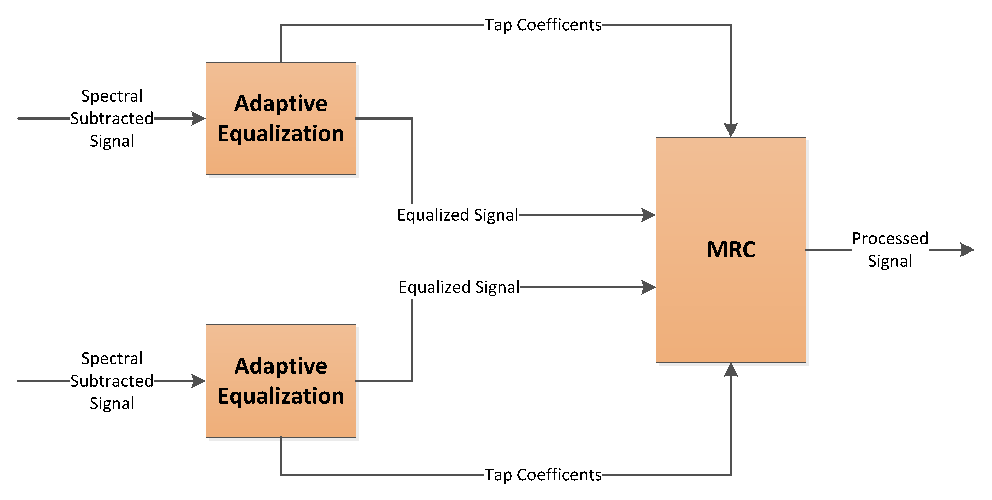
\includegraphics[scale=0.8]{mrc_sys.eps}
\caption{Maxmimal Ratio Combining Block design to replace original Super Imposed Equalizer design}
\end{figure}

\section{Antenna Subset Selection}

The Antenna Subset Selection (AntSS) block was fully contracted out to external contractors but unfortunately was never fully completed.  It is important to understand the purpose of this block for future research, and how it should iteract with the other blocks of the system.  The AntSS system itself consists of a series of AntSS boards that provides \(2^{M}$$ -to-$$2^{N}\) downselection from an array of receive antennas to a set of BLISS receiver inputs. Each individual AntSS board provides 4-to-2 antenna downselection via a set of RF switches. A basic block diagram of an individual AntSS board is given in Figure \ref{ants_sys}.  Each AntSS board has four receive paths. Each path consists of a bandpass filter and low-noise amplifier. The output of each receive path is connected to a switch matrix composed of a series of Single-Pole-Double-Throw (SPDT) RF Switches. The switch matrix is configured so that all possible permutations of the 4-to-2 downselection are possible. The switch matrix is controlled by software running on a simple PIC processor. The PIC interfaces with the BLISS hardware platform via an RS-232 link that is connected from the BLISS receiver to all AntSS boards.\\

\begin{figure}[!ht]\label{ants_sys}
\centering
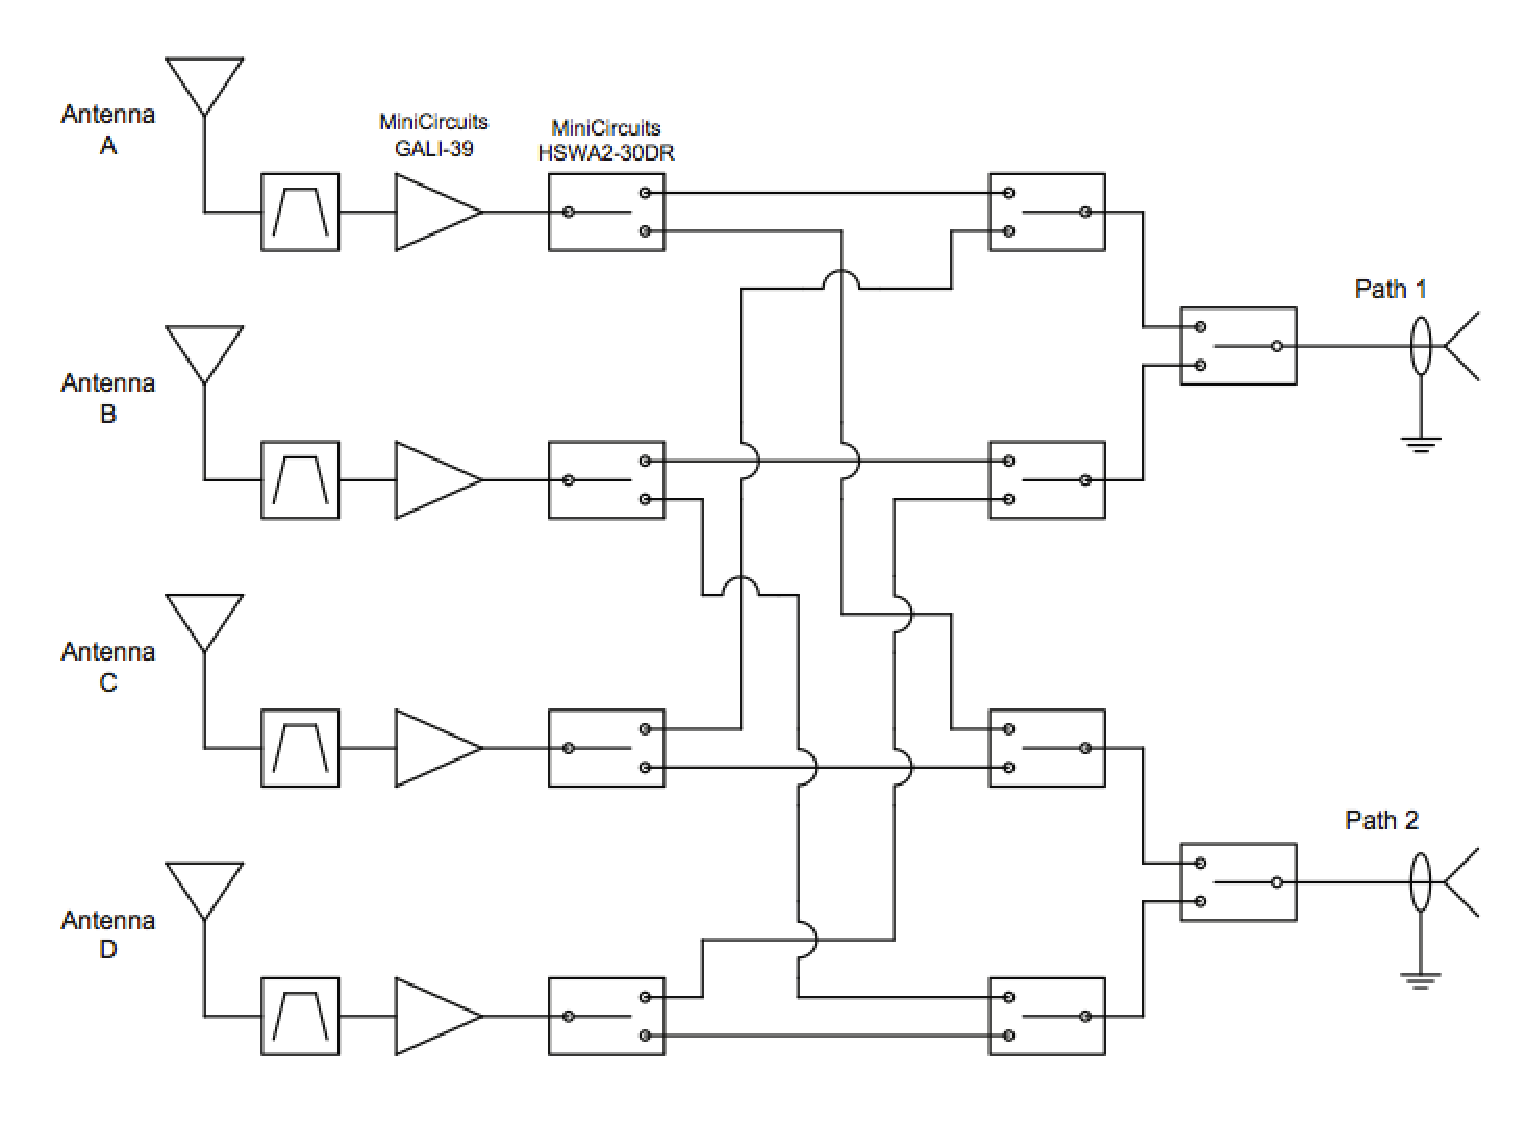
\includegraphics[scale=0.6]{ants_sys.eps}
\caption{Antenna Subset Selection block outline}
\end{figure}

During operation, training information which was used also by the signal separation block is also used by AntSS.  It uses this data to provide SNR values at each Antenna of the desired signal.  Once all antennas have been evaluated the system then selects a subset of the best antennas, which is defined by the highest SNR levels.  The signals from these antennas are then fed into the remain BLISS blocks.  AntSS can have \(2^{M}\) antennas, but will always deliever two signals.  The antennas need to be space at least a single wavelength appart or they will not be considered independent of one another, reducing the effectiveness of AntSS.  The physical boards have been built, which can be seen in figure \ref{antss_boards} and their frequency response on the individual channels can be seen in Appendix \ref{ANTSS_F_RESPONSE}.\\

\begin{figure}[!ht]\label{antss_boards}
\centering
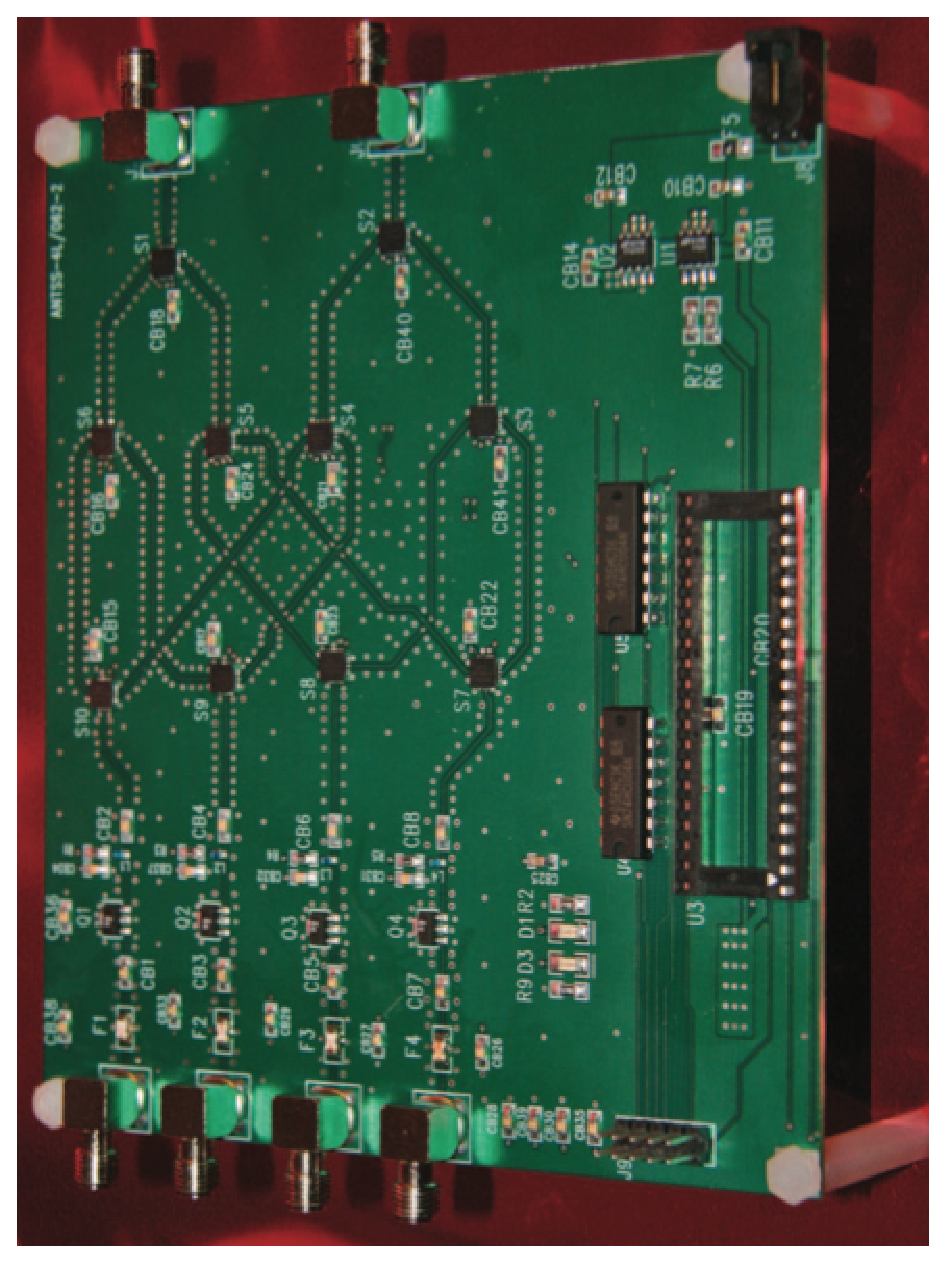
\includegraphics[scale=0.8]{ants_board.eps}
\caption{Single Antenna Subset Selection physcial board}
\end{figure}

Unfortunately none of the control mechanisms in software have been created, therefore AntSS couldn't be fully tested and effectiveness deteremined.  This will be a reasonable avenue for future work.\\

\section{Summary}

This chapter discussed the implementation fallbacks and successes of the BLISS system.  The entire BLISS system was outlined and structinized for feasilbility and operational performance.  Spectral Subtraction and Signal Separation were transitioned from original research goals to more managable problems, with simplified solutions.  Overall it can be said that optimality and technical complexity were sacrificed in the end for realiseability.  Many directions needed to be changed, especially in the Signal Separation block, and constraints needed to be tightened on the Spectral Subtraction block.  Although AntSS couldn't be realized a solid foundation exists for future work.\\ 





%\chapter{Implementation}
\label{ch:implementation}

\section{Overview}

Now that a significant background has been provided, the problem this thesis combats will be futher framed and defined.  This chapter outlines the proposed implementation of a receiver design, for wideband jammer scenarios and low-mobility situations.  An adaptive signal processing software solution for mitigating the effects of both intentional and unintentional jamming (including wideband jamming) through a combination of three techniques.  These include: antenna subset selection, spectral subtraction, and blind source separation (BSS), which work in conjuction with one another to extract specific transmissions from a mixture of intercepted wireless signals. The goal of the proposed solution, called BLInd Spectrum Separation (BLISS), is to enable reliable, high throughput, and robust end-to-end wireless communications, especially high capacity multimedia (voice, data, imagery) transmissions. In particular, the focus of the proposed work is the so-called ``disadvantaged user''.  These users are generally considered limited in transmission and processing power such as small-deck combatants, submarines, unmanned air vehicles (UAVs), dispersed ground units in urban and radio frequency (RF) challenged environments.  The previous research is also discussed for each section and implementation consideration are examined from this work.\\

The BLISS solution integrates three well-known adaptive signal processing algorithms found in the open literature: antenna subset selection, spectral subtraction, and blind source separation. Each of these algorithms is employed within the BLISS framework in order to enable the process of extracting individual transmissions intercepted from several mixtures of wireless signals. Although blind source separation can readily extract transmissions under ideal conditions, the BLISS system is aimed at harsh spectral envirnorments consisting of many users and in some cases jamming devices. Therefore BSS will not provide adiquate signal separation for robust throughput.  Hence, the other two algorithms, spectral subtractions and antenna subset selection will aid in this effort.\\

In previous sections it has been understood that current anti-jamming techniques cannot compensate in deterministic wideband jamming scenarios.  These scenarios must be throughly understood before a practical solution can be provided.  For this thesis, the worst case scenario will be considered for the jamming device.  For simplification a narrowband jammer will be considered as an adversary, and the transceiving devices cannot frequency hop thus remaining on the same frequency as the jammer.  The jammer has an identical modulation scheme as the friendly tranceivers and the constellation is in phase.  Finally the jammer is assumed at a similar distance and transmit power as the friendly tranceiving devices.  Under these conditions the jammer is completely orthogonal and historically impossible to remove.\\

This chapter is broken down into several sections which include a system level overview, the hardware and software choosen, signal removal evaluation, the superimposed equalizer design, and the antenna subset selection work.  Each of the systems that makeup BLISS have different purposes and goals allowing them to tackle different problems that occur.  It is important to note that these systems are at differing stages of development due to the limited time and initial development put into these blocks.\\ 

\section{System}

To provide a more straight forward explaination of the BLISS system it is appropriate to provided a system level overview.  The system's original purpose was to remove the effects of narrow and wideband jamming.  It accomplishes this goal through a series of processing blocks and a selection block.  These blocks include: the antenna subset selection (AntSS) block, spectral subtraction block, and finally the blind source separation block.  The figure below shows the interconnections between these blocks and certain modification were made from the original design of the system due to practical constraints.  These changes will be brought fourth as the blocks themselves are discussed in detail. Since an external research group is responsible to the AntSS block, it will not be throughly discussed by this thesis, but its fundimental purpose will be examined.\\

\begin{figure}[!ht]\label{bliss_system}
\centering
\includegraphics[scale=0.5]{bliss_system.eps}
\caption{Overview of BLISS System }
\end{figure}

The first step in the BLISS system is to pass through the AntSS block.  Physically this block is equipped with many antenna in groups of 4.  As the block title portrays a subset of these antennas will be selected and they will be passed on to the next block.  Precisely a \(2^{M}-to-2^{N}\) downselection from an array of receive antennas to a set of BLISS receiver inputs. Each individual AntSS board provides 4-to-2 antenna downselection through a set of RF switches.  The goal of AntSS is to provide spatial separation through an array of antennas maximizing the SNR of the wanted signal.  It is important to note that the antenna spacing must be adiquet to provide enough separation or independence, depending on the operating frequencies or wavelength of the signals themselves.  Once the appropriate antennas are selected two signals are to the spectral subtraction block.\\

The spectral subtraction block is next, which is used to removal known unwanted signal from the spectrum so the source separation block and work properly.  The original design of the spectral subtraction block is to use an existing audio technique of removing noise or signals in the frequency domain through a subtraction and smoothing technique.  This technique was discussed previously in the background section, therefore its historical literature will not be examined futher.  To enable removal of unwanted signals, the Spectral Subtraction block maintained a database of known power spectral densities (PSD) of common modulation schemes.  A recognition system would be implemented to automatic identification of the interfering signal and the block would simply subtract it out, through its already known estimate from its database.  Next the newly subtracted signal would be passed to the Source Separation System, where the signal would be unmixed.\\

The source separation block separates signals when only their mixtures are observed.  The operation is called blind, since the signal sources and mixing procedure are unknown to the receiver.  Under some conditions this constraint cannot be completely upheld.  This is true because the solutions needed to solve such an event become generally intractable.  An initial approach in this project was to use a technique called AMUSE (Algorithm for Multiple Unknown Signals Extraction)\cite{AMUSE}.  AMUSE works by first collecting an estimate of the covariance matrix of the received signal, computing the singular value decomposition of that covariance matrix, then performing several transforms on the received signal once the number of mixed received signals is known.  Then a covariance is calculated from these transformed received signals which are offset by some instance \(\tau\), and a eigenvalue decomposition is done upon these covariances.  From this decomposition the singular values are used with the transform matrix and the received signal to provide an estimate of the wanted source signal.\\

\begin{equation}\label{}
R_{y}=E[yy^{t}]
\end{equation}

\begin{equation}\label{}
z=Cy
\end{equation}

\begin{equation}\label{}
R_{z}=E[z(\tau)z(t-\tau)^{t}
\end{equation}

\begin{equation}\label{}
\hat{x}=Vhat{t}Cy
\end{equation}

It is important to note that for simplicity the mixing matrix for the original proposed solution involving AMUSE is generally constructed as a linear time invariant (LTI) system.  There is some activity occuring with nonlinear mixing, but that was considered outside of the scope of this problem.\\

\section{Hardware and Software Platforms}

Before any implementation was considered a platform needed to be choosen for the end result.  This selection provided the work flowpath for the implementation, eliminating many options.  As discussed in previous chapters, the end result wants to leverage the power of Software-Defined radios (SDR).  The hardware platform chosen was the USRP2 designed and built by Ettus Research\cite{USRP2Stats}.  These radios are readily available in the Wireless Innovation Laboratory and since the number of radios required for the design was still unknown, it was an obvious choice.  There are several software packages that support the USRP2 hardware and several will be examined in this chapter.\\

The USRP2 or Universal Software Radio Peripheral are intended to be a comparatively inexpensive hardware platform for software radio, and is commonly used by research labs, universities, and hobbyists\cite{wired}.  The USRP2 connects directly to a host computer through a Gigabit Ethernet link, which relays baseband sample that have been receiver or tobe translated.   The motherboard provides the following subsystems: clock generation and synchronization, FPGA, ADCs, DACs, host processor interface, and power regulation. Several of these component are seen in the image below.  These are the basic components that are required for baseband processing of signals. A modular front-end, called a daughterboard, is used for analog operations such as up and down conversion, filtering, and other signal conditioning. By replacing this RF daughtercard many different frequency ranges can be examined.\\

\begin{figure}\label{usrp2_full_hardware}
\centering
\includegraphics[scale=0.1]{usrp2_overview.eps}
\caption{Full USRP2 Hardware with Daughtercard}
\end{figure}

\begin{figure}\label{usrp2_mainboard}
\centering
\includegraphics[scale=0.1]{usrp2_mainboard.eps}
\caption{USRP2 Mainboard}
\end{figure}


The information flow is important to understand within the phyiscal radio.  This SDR block diagram shown below, outlines the common tasks done by the: daughtercard, FPGA, DAC/ADC, and host computer.  Since the FPGA is programmable the operations can change if desire, but the three dominating software packages that utlize the USRP2 flow this structure.  Beginning on the far left of the diagram and continuing to the right, at the daughtercard are RF emitions are received and transmitted.  The daughter also contain mixers that translate the signal to an intermediate frequency.  Next come the dual 100 MS/s 14-bit ADCs, dual 400 MS/s 16-bit DACs, two digital down-converters with programmable decimation rates, and two digital up-converters with programmable interpolation rates\cite{USRP2Stats}.  These are located on the mainboard of the USRP2 itself.  The FPGA is a Xilinx Spartan 3 XC3S2000, which with the current FPGA software is 59\% free in general logic but only 3\% free in memory.  The FPGA also does not have any DSP resources.  The limited memory left in the USRP2 FPGA severely limited any additional development.  As a result on newer models, such as the N210, the FPGA has been upgrade.\cite{n210spec}\\

\begin{figure}[!ht]
\centering
\includegraphics[scale=0.5]{sdr_block_d.eps}
\caption{USRP System Block Diagram\cite{sdr_blocks}}
\end{figure}

The data itself constain several pieces of metadata in a frame.  RX metadata structure for describing sent IF data includes time specification, fragmentation flags, burst flags, and error codes. The receive routines convert IF data headers into metadata\cite{metadata}.  Such metadata can be used to indicate the position and FPGA timestamp associated with the sample that corresponds to the start of the underlying frame. By default, existing blocks will transparently propagate any attributes contained on their input streams to their output streams. Blocks that use the attributes can query their input streams to locate all (key, value, offset) tuples in the region of the stream that they are currently working on in their “work” method. Likewise, blocks can copy, add or delete attributes on their output streams\cite{sdr_blog}.  This knowledge is extremely useful when doing multiple receive antenna arrays when alignment is necessary, or in any situation where fine timing information is required.\\

With the USRP hardware several software options are available including: GNU Radio, MATLAB, LabVIEW, and several custom packages.  MATLAB and GNU Radio have already been discussed, therefore the selection between them shall be discussed.  Since this system is a MIMO implementation signal alignment is a requirement.  MATLAB doesn't support sample alignment in a multiple USRP system.  The sample alignment is possible through either external means through an external clock or through the option choosen here the MIMO cable.  The MIMO cable, a picture of it can be seen in figure \ref{mimo}, is a standard 16-pole flatcable to connect tvrx, basic-rx or dbsrx boards.  Of this 16pin flatcable only two pins are used (io15 and ground)\cite{mimo_cable}.  An image also of the combined dual radio source block can be seen in figure \ref{mimo_grc} from GNU Radio.  With this requirement GNU Radio must be used for direct access with the USRP2.  Aswell full implementation of the systems blocks were first attempted with GNU Radio.  Fortunately, if necessary, data can be passed to MATLAB for signal processing from GNU Radio through the use of the file blocks and a script located in Appendix A.\\

\begin{figure}[!ht]\label{mimo}
\centering
\includegraphics[scale=0.1]{mimo.eps}%taken on iphone
\caption{USRP2 MIMO Cable}
\end{figure} 

\begin{figure}[!ht]\label{mimo_grc}
\centering
\includegraphics[scale=0.6]{mimo_grc.eps}
\caption{GNU-Radio MIMO Enable Source Block}
\end{figure} 


\section{Spectral Subtraction}

Now that the a formal system level approach has been presented and hardware setup chosen, a more detailed understanding of the blocks themselves can be examined.  The goal of the spectral subtraction block is to removal signals to allow the blind source separation block to work properly.  As discussed previously signals would first need to be identified and then removed based on information supplied in a precompiled database of known signals.  The technique to remove such signals is called spectral subtraction, which primarily takes place in the frequency domain.  This approach only relys on known PSD's of the interfering signal.  Initially this technique seemed quite sound, but futher investigation proved otherwise.\\

Initial simulations were created to examine this spectral estimation technique at RF frequencies rather than the standard audio frequencies for which Spectral Subtraction is formally used.  Only two signals were used in these simulations, both utilized the same modulation scheme and pulseshaping filters.  The signals were chosen to be non-orthoganal, since when they are orthogonal The frequency of the interfering signal was varied, and so were the oversubtraction parameter \(\alpha\) and quantization floor \(\beta\).  Through experimentation \(\alpha\) worked best at a value greater than 10, and \(\beta\) worked best between 0.05 and 0.2.  The graph in figure \ref{SS_basic} shows the bit error rate (BER) as the interferer is shifted across the wanted signal in frequency.\\

\begin{figure}\label{SS_basic}
\centering
\includegraphics[scale=0.5]{SS_basic.eps}
\caption{Original Spectral Subtraction Technique Results}
\end{figure} 

As you can see this spectral subtraction technique operates extremely poor when the signal are overlapping at all.  The reason system performs well at large frequency shifts is due to the bandpass filter which is used before the signal is quantized.  The reason the result is poor is because the estimate is largely incorrect.  Since the subtraction only utilzes the PSD's of the signals, half of the information is completely ignored.  This results in a completely inaccurate estimate.  The problem with traditional Spectral Subtraction is that its results are subjectively evaluated or done, which isn't accurate enough in a digital communication system.  Other evaluations uses such metrics as SNR, which can be quite deceptive esspecially in digital communications.  Such examples can be seen here: \cite{ss_subjective1}, \cite{ss_subjective2} \\

Since the initial simulations for traditional Spectral Subtraction proved inadiquated other optioned needed to be explored.  First though, the problem needed to be an analyzed further for better understanding, then the appropriate solution could be formulated.  Since the interfering signal and the wanted signal are non-orthoganal to one another they will share dimensional space, in this case the signals are inphase with one another.  Therefore both planes real and imaginary must be considered.  Non-orthoganal signal removal is a common task in communication system, which is done primarily by equalizers.  Therefore an equalizer approach was considered next.\\

\subsection{Equalizer Approach}

The equalizer approach used in this Spectral Subtraction approach is a Least Means Square (LMS) equalizer, utilizing training data used in the front portion of each transmitted frame.  This a common equalizer used in practice, allowing for future translation into a realized implementation.  The LMS equalizer was also chosen for it robustness no noise, which is a weakness of such equalizers as the zero-forcing equalizer and requires no matrix inversion such as the Least Square (LS) equalizer.  For proof of concept the entire datastream is used as training data, which provides the best results of any given channel for an adaptive equalizer, since the maximum knowledge is gained about the channel for each frame received.  The results below show the BER as the signals pass over one another in frequency, similar to the previous evaluation using traditional Spectral Subtraction.\\
  
\begin{figure}[!ht]\label{SS_equalizer}
\centering
\includegraphics[scale=0.5]{SS_Equalizer_sim.eps}
\caption{Spectral Subtraction Equalizer Test}
\end{figure} 

As you can see the figure above, the equalizer approach doesn't provide any improve beyond the traditional Spectral Subtraction approach.  The problem with using traditional adaptive equalizers is that they can only be used with a comparative slowly fading channel.  Since knowledge learned from the training data can be applied at the earliest to the next frame, if the interference changes enough it can render the equalizer useless.  This rapidly changing spectrum or energy within the spectrum is unforunately a common characteristic of jammers.  Even though this approach failed it provided an important observation and incite into the requirements and scenarios in which jammers can be overcome.  For the sake of completeness an additional test was done with a small repeating sequence, smaller than the equalizer tap size, and as aspected the equalizer was able to overcome the interferer.\\

%\begin{figure}\label{SS_equalizer_small}
%\includegraphics{SS_Equalizer_small.eps}
%\end{figure} 


The important conclusion drawn from the previous experiment is that the when signals are orthogonal the receiver needs to be able to predict what data or energy is being transmismitted at a given time.  Therefore the jammer problem must be constained future.  As a result two jammer scenarios will be defined.  The first scenarios is that the jammer's modulated data or energy is completely known to the receiver and the second is that the data sequence repeats with period being small.  The larger the period the more resources the receiver will need to devote to its determination and evaluation.  The sequence being completely known to the jammer is a reasonable assumption; primarily if the jammer is friendly, as discussed previously in this thesis, then that knowledge can be readily available.\\

Now that the jammer scenarios have been defined further they can be evaluated.  The first will be when the data sequence of the jammer is completely known to the receiver.  The approach here will be to synchronize with the interfering signal, so the interferer will simply be subtracted off.  To synchronize the signals a mathematical tool called correlation will be used.  Correlation is a common tool used in synchronization in communication systems when looking for known symbols in a stream of data.  Equation \ref{cross} for cross-correlation simply passes signals over one another, the resulting sequence creates peaks where the data is most correlated.\\

%\[ (f\star g)[n] = summation f^{\star}[m]g[n+m]\] NEED CITATION\\
\begin{equation}\label{cross}
R_{XY}(t_{1},t_{2})=E[X_{t_{1}}Y_{t_{2}}] \cite{gubner}
\end{equation}

An example of two sequences being cross-correlated with one another can be seen below, with the peak being where the signal line up of share the most mutual information with one another.  Therefore from this data the location of the start of the interfers data can easily be located and removed.  A simulation was created with this design in mind, with a unique result.  Since the signals are frequency shifted over one another, when there frequencies match, it produces the best result, but as soon as they are offset, errors start to occur.  This can easily be compensated for using a complex exponential multiplied by either the received or catalogued waveform.  This will enduce a frequency shift cancelling out the shifting signal.  Therefore the error is just a function of the noise itself.\\

\begin{figure}[!ht]\label{ss_correlation}
%changing power graph of subtraction
\centering
\includegraphics[scale=0.5]{ss_correlation_sim.eps}
\caption{Spectral Subtraction Correlation method}
\end{figure} 

This simulation was also repeated but this time was subtracted in the frequency domain.  The result produced near identical results.  Since using this approach requires two fourier transforms, into and out of the frequency domain, computationally it is much more involved and requires many more resources than the time domain approach.  If the data was already the frequency domain from some other process or signal processing technique then the frequency subtraction would be a viable option.\\

Further analysis was done to provide a solid understand of the new requirements of the system and its limitations.  The first is the precise understanding of the interfering signal itself.  Since it is assumed that the signal modulation and data stream is known, attention can be shifted to the other issues that can occur, which are the non-idealities of the system.  The first is the power constraint or effect.  When subtracting the interferer specific power must be measure of the interferer alone, so close to as little possible energy is subtracted from the joined signal that belongs to the desired signal.  An examination of the incorrect estimation of the interfering signal was examined in \ref{power_delta}.

\begin{figure}[!ht]\label{power_delta}  
%changing power graph of subtraction
\centering
\includegraphics[scale=0.5]{ss_conv_changing_over_subtraction_level.eps}
\caption{Spectral Subtraction Correlation Test with Varying Oversubtraction Level}
\end{figure}

Besides power, frequency and timing offsets were examined.  These are especially concerning because the signal cannot be demodulated when in operation for feedback information, because it must be fed into the signal separation block for equalization.  Therefore a timing recovery mechanism cannot downsample the signal either.  The timing recovery and carrier recovery mechanism therefore needed to be unobtrusive as possible to the signal.  As a result frequency and timing shifts were examined to understand the sensitivity of the subtraction, and how accurate the recovery mechanismed needed to be.

%Freq Shifting
\begin{figure}[!ht]\label{shifting}
%Timing (Phase) shifting
\centering
\includegraphics[scale=0.5]{ss_conv_phase_offsets.eps}
\caption{Spectral Subtraction with Phase Offsets of Interfering Signal}
\end{figure}

As you can see from figure \ref{shifting}, the subtraction mechanism is extremely sensitive to timing offsets, while frequency shifts the system is rather robust.  If a full bitshift occures though, the entire system falls apart.  This is a rather large problem and must be considered when attempting such operation on non-simulated data.  This problem was forsean because of the time variance or sensitive of the signals themselves. \\

Moving on, now that a viable subtraction technique has been determined, the final implementation for the Spectral Subtraction block can be realized.  As discussed in the Hardware and Software Platform section of this thesis, GNU Radio was the first to be examined because of its realtime attributes.  This was quite an involved process requiring many weeks of trial and error.  The first implementation was entirely written in C++, which is the recommended language for signal processing blocks in GNU Radio.\\  

Since C++ within GNU differs from many modern programming styles a code implementation or route was taken to ensure accuracy and speed up development.  Therefore all coding was done with C++ itself, using no GNU Radio built-in libraries\cite{gnuradioCPP}.  To allow for matrix operations the Aramdillo C++ Library\cite{armadillo} was imported and provided needed vector operations such as correlation and faster mathematical functions instead of having to rewrite common search operations.  This library would also be needed for the Signal Separation block, therefore coding with Armadillo would provide the knowledge for future implementations needed in that block.  From the standard C++ implementation results were compared with Matlab, and the code was ported into GNU Radio.\\

\begin{figure}[!ht] 
\centering
\includegraphics[scale=0.5]{code_work_flow.eps}
\caption{GNU-Radio Code Implementation Workflow}
\end{figure}

GNU Radio C++ are basically written by first creating test cases and writing your code until they are solved.  This is a common practice among the programming community and provides a definitive endpoint to the code itself.  The code was written and compiled successfully but unforunately the python wrapper called SWIG\cite{swig}, which GNU Radio uses to interact with the C++ block through python, was unable to export the library.  This is an undocumented problem within GNU Radio and was only identified through discussions directly with the GNU Radio core development team.  Therefore another approach had to be considered.\\

The next option was to use python itself for signal processing.  This is approach was primarily developed by Josh Blum, one of the core developer of GNU Radio.  It isn't recommended due to speed issue, but it is quite easier to implement and debug for those familiar with python.  As a result the previously C++ code was ported to python standards libraries and then to GNU Radio.  The NumPy libraries were used within python.  NumPy is the fundimental package for scientific computing in Python\cite{numpy}.  It like the armadillo library provides matrix operations such as correlation.  Again under the Python standard libraries with NumPy the results were varified with MATLAB.  Then the code was port to GNU Radio.\\

Again more problems occured, stonewalling all progress.  The signal processing block was written as a subprocess using the queuing system built into GNU Radio.  Queueing provides barriers between the connected blocks; therefore they can run freely, limiting bottlenecks. The system built would operate correctly for several hundred samples but would eventually segmentation fault.  Several attempts to fix this error with even architectural changes to the code.  Finally the lead developer of GNU Radio was consulted, Tom Rondeau \cite{tomrondeau}, but he was also unable to determine a solution.  The assumed problem was a type casting occuring within the queue itself, that would eventually accumulate and cause a segmentation fault.\\

With these setbacks, it became necessary to look beyond GNU Radio and just utilize MATLAB for signal processing.  Therefore the decision to load captured signals from GNU Radio and process them in MATLAB.  It is nowhere near realtime, but it will process the data appropriately.  The simple GNU Radio needs frontend is important because it allows tight synchronization between multiple receive antenna, which is a require of the original design of the system.  The GNU Radio model can be seen in figure \ref{grc_receiver}, the modulator block has been customized to remove the quantization, producing floating point results.\\

\begin{figure}[!ht]\label{grc_receiver}
\centering
\includegraphics[scale=0.5]{grc_receiver.eps}
\caption{GNU-Radio Receiver Half Design}
\end{figure}

\subsection{Non-deterministic Scenarios}

For completeness it is important to discuss the scenarios when the interferer's modulated data is unknown but repetative with a small period.  The approach to estimating short sequences is a rather obvious one, an autoregressive algorithm is used to predict samples.  The simulation here, which was just used for proof of concept, uses a linear predictive filter.  The filter determines coefficients of a forward linear predictor by minimizing the prediction error in the least squares sense\cite{lpcfilter}.  It finds the coefficients of a pth-order linear predictor (FIR filter) that predicts the current value of the real-valued time series x based on past samples.

\[ \hat{x}[n]=-a(2)x(n-1)-a(3)x(n-2)-...-a(p+1)x(n-p)\]

For the linear predictive filter to operate efficently the number of filter taps must be equal to or greater than the period of the repeated sequence.  If the number of taps is smaller it cannot capture the randomness the in the interferer's data.\\

\subsection{Over the Air Implementation Considerations}

When moving towards a real implementation of the Spectral Subtraction block, the non-idealities introduced by the envirorment needed to be considered.  These include frequency and phase shifts, as well as timing offsets.  Certain considerations needed to be made as well, since instanteous changes occur when signals overlap.  Therefore a more advanced control scheme needed to be constructed around the common signal compensation or correction.  The basic idea used here is a receiver within a receiver, one for each signal received.  This will be discussed in detail.\\

The system assumes that the jammer is always present within the envirorment therefore it was concluded that the jamming signal should be synchronized with first, be removed and then all that remains should be the wanted signal.  There is were the receiver within a receiver design comes in, since first the interferer will be synchronized to, utilizing phase and frequency recovery and then timing recovery.  Unforunately such an implementation isn't as straight forward as expected.  Since when both signal are present in the spectrum it is impossible for these algorithm to operate correctly.  This is due the fact that they cannot separate one signal from the other.  For example, phase information cannot be accurately calcuated in the presence of two signals.  Therefore modifications need to made, which is where a controlling mechanism comes into play.\\

When multiple signals are in the envirorment the compensation algorithm learn incorrectly; as a result, a decision was made to pause these algorithms when both signals were present and continue when the signal interferer was only present.  This operation relys on two assumptions, the first is that both signals are present for short periods of time which can be controlled.  The second is that the calculated offsets of cause by the envirorment don't rapidly vary during the periods of time for which the two signals are visible.  This assumption is quite reasonable especially with relatively non-mobile transceivers, which was assumed in the original documentation.\\

To accomplish this algorithm holding mechanism, energy detection was chosen to be uses for its simplicity.  Below you can see an image of the jammer signal by itself and the combined signals.  A large increase in energy or step can be seen, which can easily numerically detected.  Energy is calculated using the following equation: \(E_{s}=\newcommand{\inftyint}{\int_{-\infty}^{+\infty}}|x(t)|^{2}dt\).  This was implemented with a moving average filter with a small window to reduce sperious changes due to signals gaps or outliers.  In practice the average peak energy level of the interferer is first calculated, then when the power in the spectrum increases to a level roughly 1.5x of the original level, the compensation algorithms are halted.  A simple technqiue technique, which is commonly uses but in the inverse fashion.  An example of the combined and signals can be seen in figure \ref{combo_signal_time}.  The final results of the Spectral Subtraction block are examined in the next chapter.\\


\begin{figure}[!ht]\label{combo_signal_time}
\centering
\includegraphics[scale=0.5]{combo_signal_time.eps}
\caption{Received mixed and individual signals}
\end{figure}

\section{Superimposed Equalizer}

Moving on, the next block to discuss is the signal separation block.  The development of this block is very staggered and due to time requirements shortcuts needed to be made.  The original desired result was to use a blind source separation technique outlined here \cite{AMUSE}, which is able to separate multiple signals from one another under specific constraints.  For this process to work efficently an appropriate channel model needs to be created.  Since the goal of this system is to be very robust an estimator for very frequency selective channel is desired.  The progession of the signal separation block will be examined in this sections and the limitations will be discussed.  It is important to note that a large variation was taken in the system design due to implementation feasibility.\\

The original objective was the utilize a new signal separation technique called AMUSE, but a new avenue was taken with a more theoretical channel estimation problem in mind.  This estimation evaluation will be discussed first.  The first objective for channel estimation is to examine the channel mixing model which assumes a single-input multiple-antenna broadcast channel.  A J-channel FIR system excited by K transmit antennas is considered. A quasi time-invariant multipath channel is assumed which remains constant during the transmission of a set of consecutive symbols, which are called slots. These slots are assumed independent from one another.  The channel estimation is performed over each slot. Each symbol inside a slot is assumed to be the result of a known redundant precoder acting on an input transmit symbol vector drawn from an M-PSK constellation. Therefore the receiver receives signals not only from the intended transmitter but also from Q other interferers. The interferers are assumed to employ the same redundant precoder as the desired signal\cite{skrkantPHD}.\\

With this model, \cite{midterm_report} shows that no assumptions are necessary regarding the number of the transmit antennas of each of the interferers and the channel orders as long as they are smaller than the block size.  The block size in this case is equal to the combination of the individual channel lengths and the number of transmit antenna used by the desired transmitter.  But this evaluation rely on three assumptions:

\begin{enumerate}
\item The data sequence \(x_{d}\) is an i.i.d. sequence such that \(x_{d}\sim\mathcal{CN}(0,\sigma_{d}^{2})\)

\item The distribution over the MIMO channel vector is \(p(y;\theta)\sim\mathcal{CN}(\mu_{y},R_{w})\), and the interference vector is distrbuted normal with covariance \(R_{w}\)

\item The transmitted symbols, the channel vector, and the interference vector are jointly independent
\end{enumerate}

With these assumptions the mixing process can be undone but the channel estimation needs to be calculated first.  Since this is a MIMO channel, frequency selective fading will need to be captured to providing appropriate channel knowledge.  To accomplish this, the original research decided to utlize superimposed equalization, whose operation was heavily discussed in the background section of this thesis.  In summary, \cite{Ghogho} uses a superimposed symbol transmission scheme to estimate frequency-selective channels. Several points of the DFT of the data are set to known values. This operation can be easily implemented in the time domain when these DFT points are equispaced. The channel is estimated using the DFT of the received signal at these selected DFT points. The detection itself is done using an iterative method across these points.  Unlike traditional equalizers, the proposed method does not require bandwidth for training.  It instead trades spectral power for those symbols themselves, spreading its energy over the entire bandwidth capturing the entire spectrum space.   \cite{Ghogho} also proves that by placing the training symbols in quasi-periodic position they will not interfer with the data itself.  It is important to note that this research discusses no sychronization mechanism, and now with the training data spread throughout the signal is very complex.  This addition complexity was factored into the design decisions of the implementation, which is discussed later in this section.\\

With our channel estimation method chosen, a simulation was created to prove the effectiveness of such a scheme.  The result of this implementation were directly compared with the results of the paper to prove correctness.% and compared with traditional equalizer performance&
The results of this simulation are seen in figure \ref{sie}.  It examines a random frequency selective channel, with very high suppression with a across a number of SNR values.  As expected there is a linear relationship between SNR and Error.\\  %For completeness a comparision was done with a traditional LMS equalizer to show the effectiveness of the superimpose equalizer.\\

\begin{figure}[!ht]\label{sie}
\centering
\includegraphics[scale=0.5]{sie_SNR.eps}
\caption{Superimposed Equalizer SNR Performance}
\end{figure}

\begin{figure}[!ht]\label{sie_freq}
\centering
\includegraphics[scale=0.5]{freq_response_sie.eps}
\caption{Superimposed Equalizer Channel Estimation Performance with High SNR}
\end{figure}

%INSERT Figure of SNR and channel estimate for Superimpose equalizer\\
%
%INSERT Figure with comparision of superimposed equalizer vs. traditional linear equalizer\\

From figure \ref{sie_freq} you can see in a frequency selective fading channel is very well estimated by the superimposed equalizer.  This was exactly the result that was desired, but symbol recovery after equalization still needed to be examined. This unfortunately is the drawback of this formulation.  The first is the condition if the mixing matrix \(H\) is rank deficient, the channel become inestimiable,  since there become an infinite amount of solutions to the actual unmixing process.  The second is the equalizer, which is numerically intensive, and the alternative has limiting conditions \cite{Ghogho}.  This conclusion, which isn't discussed in \cite{Ghogho}, is when the equalized signal is very suppressed due to the incomplete channel estimate.  The quantization feedback method overcome the previously received frame and dominated all future frames, essentually neglecting any information they have.  Again this only in very suppresive channels.  With these results the superimposed equalizer started to become less desirable due to it's complexity, but evaluations continued due to the amount of time invested into the topic already.\\

%NEED MORE MATHEMATICAL EXPLAINATION 


%%%%%%%%%%CONTINUE EDITING
%%%%%%%%%%CONTINUE EDITING
%%%%%%%%%%CONTINUE EDITING

These simulations provide the necessary foundation to push towards the final implementation of the signal separation block.  However, due to time constraints certain decisions needed to be made about this block and the feasibility of its operation.  With that in mind the primary goal for the signal separation block was to provide signal separation or maximization from several received signals.  Since the previous research provided substantial implemenation considerations and issue, a new direction needed to be considered.  Therefore instead of the proposed AMUSE\cite{AMUSE} technique, another MIMO cross-channel technique called Maxmimal Ratio Combining (MRC) was chosen as a viable alternative.  This decision was made with both project managers.\\

Maximal Ratio Combining is a method of diversity combining in which the signal add first weighted and then added together.  These weights or gains are made proportional to the RMS signal level and are inversely proportional to the mean square noise level in that channel, and the same proportionality constant is used for all channels\cite{fs1037c}.  Therefore the channel with the best SNR provides the greatest impact on the resulting sequence.  This process needs to explain more throughly.  Assuming the received signal is an array of samples received the individual antennas \(\boldsymbol{x}(t)=\boldsymbol{h}(t)u(t)+\boldsymbol{n}(t)\) and the individual channels \(\boldsymbol{h}=[h_{0},h_{1},...,h_{N-1}]^{T}\), and the additive noise \(\boldsymbol{n}=[n_{0},n_{1},...,n_{N-1}^{T}\).  The equalized symbol \(\hat{x}=x+(h^{H}n)/(h^{H}h) \) \cite{diversity}.

A simple evaluation of MRC was done to prove its capabilities, which is based on the simulations here \cite{mrc_m}.

\begin{figure}[!ht] 
\centering
\includegraphics[scale=0.5]{mrc_gain.eps}
\caption{Maximal Ratio Combining gain acrossing varying number of antennas}
\end{figure}

As you can see as you increase the number of antennas in a frequency selective channel the better the result.  Therefore MRC was introduce into the framework of the signal separation block, and the new model for this block can be seen in figure \ref{mrc_sys}.  This block first utlizes adaptive equalizers on the channels individually then uses MRC to combine there results maximizing the SNR of the desired signal.  MRC was combined with the channel estimate approach using adaptive equalizers due to there known feasibility.  From the knowledge learned in the previous with the implementation involving GNU Radio, the signal separation block was created entirely in MATLAB.  The results of this operation will be discussed in the final chapter of the thesis.\\

\begin{figure}[!ht]\label{mrc_sys}
\centering
\includegraphics[scale=0.8]{mrc_sys.eps}
\caption{Maxmimal Ratio Combining Block design to replace original Super Imposed Equalizer design}
\end{figure}

\section{Antenna Subset Selection}

The Antenna Subset Selection (AntSS) block was fully contracted out to external contractors but unfortunately was never fully completed.  It is important to understand the purpose of this block for future research, and how it should iteract with the other blocks of the system.  The AntSS system itself consists of a series of AntSS boards that provides \(2^{M}$$ -to-$$2^{N}\) downselection from an array of receive antennas to a set of BLISS receiver inputs. Each individual AntSS board provides 4-to-2 antenna downselection via a set of RF switches. A basic block diagram of an individual AntSS board is given in Figure \ref{ants_sys}.  Each AntSS board has four receive paths. Each path consists of a bandpass filter and low-noise amplifier. The output of each receive path is connected to a switch matrix composed of a series of Single-Pole-Double-Throw (SPDT) RF Switches. The switch matrix is configured so that all possible permutations of the 4-to-2 downselection are possible. The switch matrix is controlled by software running on a simple PIC processor. The PIC interfaces with the BLISS hardware platform via an RS-232 link that is connected from the BLISS receiver to all AntSS boards.\\

\begin{figure}[!ht]\label{ants_sys}
\centering
\includegraphics[scale=0.6]{ants_sys.eps}
\caption{Antenna Subset Selection block outline}
\end{figure}

During operation, training information which was used also by the signal separation block is also used by AntSS.  It uses this data to provide SNR values at each Antenna of the desired signal.  Once all antennas have been evaluated the system then selects a subset of the best antennas, which is defined by the highest SNR levels.  The signals from these antennas are then fed into the remain BLISS blocks.  AntSS can have \(2^{M}\) antennas, but will always deliever two signals.  The antennas need to be space at least a single wavelength appart or they will not be considered independent of one another, reducing the effectiveness of AntSS.  The physical boards have been built, which can be seen in figure \ref{antss_boards} and their frequency response on the individual channels can be seen in Appendix \ref{ANTSS_F_RESPONSE}.\\

\begin{figure}[!ht]\label{antss_boards}
\centering
\includegraphics[scale=0.8]{ants_board.eps}
\caption{Single Antenna Subset Selection physcial board}
\end{figure}

Unfortunately none of the control mechanisms in software have been created, therefore AntSS couldn't be fully tested and effectiveness deteremined.  This will be a reasonable avenue for future work.\\

\section{Summary}

This chapter discussed the implementation fallbacks and successes of the BLISS system.  The entire BLISS system was outlined and structinized for feasilbility and operational performance.  Spectral Subtraction and Signal Separation were transitioned from original research goals to more managable problems, with simplified solutions.  Overall it can be said that optimality and technical complexity were sacrificed in the end for realiseability.  Many directions needed to be changed, especially in the Signal Separation block, and constraints needed to be tightened on the Spectral Subtraction block.  Although AntSS couldn't be realized a solid foundation exists for future work.\\ 






%% Results Section
\chapter{Results}
\label{ch:results}

\section{Overview}

This chapter outlines the outcomes of the individual AS\textsuperscript{6} system blocks and evaluates their performance and realisability.  Since a large transition was made from original research and goals, many limitations were enforced in the final design presented in this thesis.  Feasibility was desired during the implementation stage of this work, causing this transition, but physical implementations were produced and analyzed.  Since certain channel conditions couldn't be replicated in reality baseline evaluations were produced for proof of concept, and rigorous hardening is a viable path for future work.\\ 

\section{Spectral Subtraction}

The goal of this section is to present the results of the Spectral Subtraction signal processing block.  This block, as mentioned in previous sections, tries to remove non-orthogonal known signals from the spectrum that are located on the same frequency of the desired signal.  Since the receiver isn't allowed to move to other bands, this mimics the effects of a wideband jamming system, causing all effective bandwidth or throughput to diminish.  From the theoretical simulations it is possible to remove the interfering signal but only under severe limitations or constraints.  The primary issue is that the signal is extremely time varying and alignment is quite difficult.  To be precise, this block tries to align a source signal with the received signal, and then subtract that signal from all future received segments. This alignment is difficult because the received signal is corrupted by noise and the channel which it passes through. That corruption is time varying as well, and difficult to model over many frames to provided sufficient signal removal.  In order to operate, this system assumes the interferer's system is completely known, including the data that is being modulated into the spectrum.  Therefore it is the goal of the Spectral Subtraction block is to regenerate the corruption caused by the channel, apply that to the source signal, and then subtract.  The experimental evaluation is outlined next and the analysis of its performance.\\

\subsection{Experiment}

This experiment consists of four USRP2 radio transceivers.  One radio acting as a transmitter, one the interferer, and two receive radio connected through a MIMO-USRP cable.  The cable causes direct synchronization between the receive radios.  This is required to perform maximal ratio combining to correctly align signals constructively.  During testing, the interferer first begins transmitting data, then the desired transmitter begins to transmit.  At all times the receiver is actively receiving all signals in the spectrum.  A sample of the combined received signals can be seen in figure \ref{combo_time_signals}.  The lower energy sections represent the individual signals and the high energy level sections show the mixed signals.\\

All transmissions utilize GMSK, due to its resilience to changes in the radio's power amplifier.  All radios operate at 100kbits/sec, well under the maximum rate of the radios, minimizing the load on the machines themselves and the amount of data generated.  The machines connected to the radios are all have Core Series Intel processors, installed with Ubuntu Linux 10.10 and 12.04.  All machines were also running MATLAB 2011B, and GNU-Radio 3.6.2git-145-g7c8347ca built from the git repository.  All signal recordings/reception was done in GNU-Radio and all signal processing at baseband was done in MATLAB.  Figure \ref{ss_setup_real} is a picture of the experimental setup with all four radios

\begin{figure}\label{ss_setup_real}
\centering
\includegraphics[scale=0.1]{ss_setup_real.eps}
\caption{Spectral Subtraction Hardware Setup}
\end{figure}

\subsection{Analysis}

The system was able to correctly identify power changes in the signal and provide the most accurate estimates before the signals begin to mix.  This mixing of signals cannot last for long periods of time because the non-idealities of the hardware and environment begin to corrupt the estimate of the interfering signal.  This corruption remove any hope of desired signal recovery.  The corruption can be seen clearly in figure \ref{ss_oscillation}, as the frames further from the estimate become more and more corrupted.  This period of time for which the estimate provides enough accuracy for spectral removal depends on the changes in phase frequency and channel effects.\\

Many of the non-idealities associated with Spectral Subtraction were discussed in the Implementation chapter.  Though most of effort was put towards compensating for these effects, they still produced a large amount of error in the final design.  These sources of corruption manifested as several different errors in the output of the block.  The first was timing offsets.  Since the interferer is extremely time-varying, if a single bit is missed, the entire signal downstream becomes corrupted.  If this timing is out of phase \(\pi\) radians, then an identical corruption occurs.  As \(\phi->0\), this exponentially decreases the error.  As for carrier frequency and phase offsets, this error manifests as an oscillating error in the output signal.  Figure \ref{ss_oscillation} shows severals frames and the resulting energy left behind after subtraction.  This plot was generate by a simplified test, just the interferer transmitted data and attempts were made to nullify these transmissions.  These oscillations point towards problems in phase or frequency estimations.\\

\begin{figure}\label{ss_oscillation}
\centering
\includegraphics[scale=0.5]{ss_oscillation.eps}
\caption{Error Oscillation After Spectral Subtraction}
\end{figure}


%%To evaluate the Spectral Subtraction block the signal was demodulated, timing recovered, and compared against the transmitted data.  Mueller Muller timing was used as a timing recovery method.  Several runs were made, and varying results were recorded.  Even with perfect knowledge of the exact modulated data, the corruption caused by the environment proved extremely hazarous to the signal.  Since the frequency drift of the USRP2 crystal oscillators, which control the transmission and reception frequencies, can vary on the order of kilohertz.  %%
These non-ideality seemed to be the most difficult problem to compensated for, and become worse when the signals are mixed.  This is because they cannot be directly measured.  A oscillating error in the spectrum, shown in figure \ref{ss_oscillation}, mirror the effects shown in the simpler nullifying case.  As express previously, Spectral Subtraction is very susceptible to data corruption.  It is analogous to hitting a moving target, since the operation is extremely time varying and time dependent.\\  

To help compensate for these non-idealities phase synchronization and carrier synchronization was attempted with the received signal.  As outlined in the Implementation chapter, Spectral Subtraction is designed as a receiver in a receiver system.  The front received locks onto the interferer, applies necessary phase shifts, and subtracts a synthetically generated signal from the previously known data which has also been modulated and pulse-shaped.  Unfortunately this the received data also contains many other effects cause by the channel, including multipath and large amounts of noise.  To resolve this the front receiver must estimate the channel and apply the same amount of noise to the signal to remove it sufficiently.  \( \bf{Y}=H_{I}(X_{I})+H_{D}(X_{D})+W \), only \(\bf{X_{I}}\) is known in this realization, and both \(\bf{H_{I}}\) and \(\bf{W}\) are time dependent.  As mentioned previously SS is very susceptible to any carrier, power, and timing effects.\\


It is important to show Spectral Subtraction operating correctly and when errors occur in the estimation.  Figure \ref{ss_result_great} show a desired result from Spectral subtraction when all timing is aligned, while figure \ref{ss_result_bad} shows the error propagation through the frames.  Both these results looked 20 frames ahead of the section used for subtraction.  Finally figure \ref{many_frames}, shows the error associated with increasing the frames looking ahead.  As expected, the further you move away from your original subtraction frame, the worse your results become.\\

\begin{figure}\label{ss_result_great}
\centering
\includegraphics[scale=0.7]{ss_result_GREAT.eps}
\caption{Desired result after Spectral Subtraction with 20 Forward Frames}
\end{figure}

\begin{figure}\label{ss_result_bad}
\centering
\includegraphics[scale=0.7]{ss_result_BAD_Timing.eps}
\caption{Error after Spectral Subtraction with incorrect phase estimates with 20 Forward Frames}
\end{figure}

\begin{figure}\label{many_frames}
\centering
\includegraphics[scale=0.7]{many_frames.eps}
\caption{Error associated with increasing duration of estimation frame}
\end{figure}


%Since noise couldn't be varied in this implementation for direct comparision against simulation, presented is a series of runs and their coinciding errors.  Each run only represents the periods for which the signals are mixed, which is roughly 3 seconds.  The error represents the accuracy of the demodulated signal and not the amount of unwanted still existing in the channel, since it is less desired.  This data can be seen in figure \ref{ss_error_runs}.\\

%\begin{figure}\label{ss_error_runs}
%\includegraphics{ss_error_runs.eps}
%\end

\subsection{Summary}

Spectral Subtraction in a extremely well studied area in signal processing, but no existing literature exists for its application in a digital communication system.  It has been shown here that it can be quite difficult for it to be applied, even under serious constraints.  Under the conditions of this thesis, the assumptions are quite reasonable, but due to the large amount of error in the results, more may need to be considered.  These may include accuracy requirements for physical equipment, primarily to reduce carrier frequency drift.  Burst scenarios may also be considered to reduce bit error rate.  Overall, for a completely non-existent field of study, these results point the possibility of operational success.  Future work will we required, especially during the implementation phase of designs.\\

\section{Signal Separation}

The Signal Separation block changed the most from the original research design.  Much of the design needed to be reconsidered because of time constraints and lack of robust research conclusions.  The design distilled down to a combination of Maximal Ratio Combining and adaptive equalization.  Two well know concepts in communication system design, and rather straight forward to implement.  Maximal Ratio Combining provides the benefits of maximizing the spectrum spatially, while also adaptively equalizing these separated data streams to help remove corruption left over by spectral subtraction of the channel itself.  The more dimensionality that can be exploited the more performance can be extracted.\\

\subsection{Experiment}

Signal Separation utilized an identical setup as the Spectral Subtraction testing, which is quite obvious since Signal Separation is downstream from Spectral subtraction in the data path.  The interferer was also removed from this testing, and the noise that pre-existed in the spectrum used to reflect the noise remaining from Spectral Subtraction.  This decision was made to separate problems or issues with the performance of the Spectral Subtraction block, providing direct analysis and evaluation of the Signal Separation block.  It takes in two data stream, which have been timing synchronize through the use of the MIMO USRP cable.  These streams are equalized by an LMS Adaptive equalizer of length 14.  These taps provided the Maximal Ratio Combining weight analysis, providing information on which of the channel was less corrupted.  This is done by combining the filter tap values and taking the ratio of the two equalizers, and these weights determine how much of each signal is added to the final output signal.\\ 

Again all transmissions utilize GMSK, due to its resilience to changes in the radio's power amplifier.  All radios operate at 100kbits/sec, well under the maximum rate of the radios, minimizing the load on the machines themselves and the amount of data generated.  The machines connected to the radios are all Core Series Intel processing, installed with Ubuntu Linux 10.10 and 12.04.  All machines were also running MATLAB 2011B, and GNU-Radio 3.6.2git-145-g7c8347ca built from the git repository.  All signal recordings/reception was done in GNU-Radio and all signal processing at baseband was done in MATLAB.  Therefore the entire Signal Separation block resides in MATLAB.\\  

Several separate transmissions were made and baseline bit error rates were calculated.  This was done by quantizing the final output and comparing the results.  The Mueller Muller method again was used for timing recovery due to its robustness.  It doesn't account for bit slips, but due to the rather short periods of transmission these can be ignored.  Since this block is designed to help in rather noisy and localized corruption situations, it can be very hard to test because there is no control over the spectral environment to set such conditions.  Rather this design shows a proof of concept with just SDR technology.  The results for the baseband tests are shown in figure \ref{ssep_snr_tests}.\\

%\begin{figure}\label{ssep_results}
%\includegraphics{ssep_results.eps}
%\caption{Implementation Signal Separation Performance with varying TX gain}
%\end{figure}

\subsection{Analysis}

From the results seen from the baseline testing, reception seems to be quite reasonable given the inferior hardware. To provide a comparison to the simulated results, the transmitter power was lowered to synthetically reduce the SNR of the signal.  The results of these tests can be seen in figure \ref{ssep_snr_tests}.   

\begin{figure}\label{ssep_snr_tests}
\centering
\includegraphics[scale=0.5]{mrc_snr_comp.eps} %{ssep_snr_tests.eps}
\caption{Implementation Signal Separation Performance with varying TX gain}
\end{figure}

Since only antennas are provided by the AntSS block, MRC will suffer.  Higher performance will be provided by more input signals, but that would increase the complexity of the system significantly.  More input signals could be a future alley for BLISS system for future research.  For the current system architecture the results are acceptable given the limitations and variability in the hardware itself.\\

\section{Antenna Subset Selection}

Since Antena Subset Selection was done by outside contractors, no analysis will be provided by this thesis.  

\section{Summary}

These results show that it is extremely difficult to avoid a wide-band jammer even when fine details are known about the interferer itself.  Spectral Subtraction has large downfalls in its implemented realization due to its fragile nature.  Small non-idealities can cause large errors, especially in timing, causing a large misalignment in the subtracted signal.  Equipment with higher tolerances would be a way of minimizing these effects.  Signal Separation is focused in solid theoretical foundation and provides additional SNR above single antenna reception, allowing an extrapolation in the dimensionality of the environment and the signal itself.  It was fully implemented with reasonable BER given the non-ideal hardware.  Additional antennas should be considered for further gains from Maximal Ratio Combining.\\






%% Conclusions Section
\chapter{Conclusions}
\label{ch:conclusions}

This chapter summarizes the work performed as part of this project and then suggests related research that can be performed in the future. The research achievements includes a description of the system developed, the capabilities of the system and the results it produced. The future work section includes a list of improvements that can be made to the system and some ideas that can start future research projects.\\

\section{Research Outcomes}

As part of this research effect, the following was achieved:

\begin{itemize}

\item The tasked original proposed research was examined and evaluated. Synthesizing several years of development and work from many individuals.

\item A viable solution was theoretically developed for the removal of non-orthogonal wide-band jamming sources.  Conservative constraints were applied to the construction, providing enough flexibility for hardware implementations.  The constraints only limited the interfering signal, determining that it must repeat in a relatively short period.  This made it more easily implementable and simplify the receiver design.  This constraint can be removed, but more resources will be required during subtraction, especially in memory resources.

\item A hardware implementation was produced for Spectral Subtraction utilizing both GNU Radio and MATLAB.

\item The proposed Spectral Subtraction block provided significant signal removal of actual over the air signals, but timing issues still remain.

\item In-depth analysis was provided into the sources of error with the Spectral Subtraction block.

\item An alternative solution was provided for the Signal Separation block originally presented.  This solution was based on a well know method, Maximal Ratio Combining, for combining signals in a constructive way by utilizing their dimensionality.  This decision was made in combination with the project advisors.

\item Theoretical simulations were generated in MATLAB providing a basis for performance for Maximal Ratio Combining.

\item A hardware implementation was produced for the Signal Separation block utilizing both GNU Radio and MATLAB.

\item A comparison was provided between the theoretical simulations and the hardware implementation.  It is unfair to directly compare the implementation and theoretical results, since the theoretical results don't account for the non-idealities associated with over the air transmissions but the comparison was provided. 

\end{itemize}

\section{Future Work}

Future research activities that are related to this work are discussed in this section.

\begin{itemize}

\item Removal of the short repeated signal constraint must be explored to not hinder the effects or purpose of the jammer itself.  Long sequences or a method for sequence generation such as LFSR (Linear Feedback Shift Registers) could be implemented in such a way.  The receiver must be able to very accurately predict what sample will come next in the stream itself in-order to provide accurate signal removal.

\item Original theoretical derivation in \cite{skrkantPHD} for Signal Separation must be readdressed and superimposed equalizer design explored.  The end resulting work focused on the effectiveness of specifically designed training data using a affine precoder.  A complex timing recover will need to be constructed to utilize such a system due to the scattered nature of the training symbols superimposed on the data itself.

\item A larger number of signals feed into the Spectral Subtraction and Signal Separation blocks should be explored to improve the functionality of Maximal Ratio Combining.

\item GNU Radio controlling blocks for Antenna Subset Selection block should be implemented to provide the necessary dimensionally separated signals into the downstream blocks.

\item System integration needs to be done between all three blocks to provide a complete system.  Performance metrics should be evaluated on this system once constructed to determine its effectiveness under wide-band jamming conditions.

\item Current implementations need to be optimized and code re-factored allowing for better code portability and performance gains.

\item Hardware considerations need to be addressed, determining requirements for actual deployment of such a system in the field.  Hardware constraints will be the largest limiting factor, especially on the RF front end of the design.



\end{itemize}

%\label{ch:conclusions}

%Just a small section for part of the background of my research. \cite{bibtexcite}

%This is the end of my paper.

%%%%%%%%%%%%%%%%%%%%%%%%%%%%%%%% THE FINISH %%%%%%%%%%%%%%%%%%%%%%%%%%%%%%%

%\appendix

% BIBLIOGRAPHY STUFF...
%\nocite{*}
%bibliography stuff

%SEE HERE for BIBTEX styles: http://www.cs.stir.ac.uk/~kjt/software/latex/showbst.html

\bibliographystyle{amsplain}
%\bibliographystyle{plain}

\bibliography{mybib}

\end{document}


%useful links:
%latex VS pdflatex : http://www.andy-roberts.net/misc/latex/pdftutorial.html
%basic intro to latex: http://www.andy-roberts.net/misc/latex/latextutorial1.html
%collection of latex links: http://www.andy-roberts.net/misc/index.html
%collection of math symbols: http://www.comp.leeds.ac.uk/andyr/misc/latex/tutorial9/symbols.pdf
%latex matrix examples: http://www.physicsforums.com/showthread.php?t=146358

%lgrind binary for Macintosh:
%https://netfiles.uiuc.edu/galanaki/www/Hints.html
% (place lgrindef in same directory as *.tex, place lgrind in /usr/local/bin

